%===============================================================================
% Template Name:      SUnORE Starter Thesis/dissertation template
% Template URI:       http://sunore.co.za/sunore-thesis/
% Description:        Starter Thesis/dissertation template for SUnORE
%                     Department of Industrial Engineering,
%                     Stellenbosch University
% Version:            1.2.1
% Author:             Dr. Martin Kidd
% License:            MIT License
% License URI:        http://opensource.org/licenses/MIT
%===============================================================================
\documentclass[msc]{thesis}
% Thesis options are:
%              skripsie
%              meng
%              msc
%              mcomm
%              phdsc
%              phdcomm
%=================================================
% add packages as needed (check first, the thesis
% class already includes some packages)
%=================================================
\usepackage[figuresright]{rotating}
\usepackage{blindtext}
\usepackage{amscd,amsmath}
\usepackage{amsfonts}
\usepackage{amssymb}
\usepackage{enumitem}
\usepackage{hyperref}
\usepackage{float}
\usepackage{verbatim}
\usepackage{multirow}
\usepackage{rotating}
\usepackage{adjustbox}

%=================================================
% thesis details
%=================================================
\thesistitle{Using complex network analysis for fraud prevention}
\student{Gustav Oosthuizen}
\graduation{March}
\gradyear{2022}
%=================================================
% if masters or skripsie
%=================================================
\supervisor{Dr. Ettienne Pienaar}
%\cosupervisor{Dr. Pieter Cloete}  % remove if NA
%=================================================
% if phd
%=================================================
\promoter{Promoter name}
\copromoter{Co-promoter name}      % remove if NA
%=================================================

% Note: If refrences does not show up press F6+F11+F6+F6+F7 in the seq specified.
\addbibresource{bibliography.bib}     % .bib file


%=================================================
% Special Math functions
%=================================================
\newcommand{\blokkie}{\hspace{.07cm}\Box\hspace{.07cm}}


\begin{document}
\SetKwInOut{Input}{Input}
\SetKwInOut{Output}{Output}


%=================================================
% front page and decleration page - were set up
% according to university standards (as specified
% in yearbook) and may not be edited
%=================================================
\frontpage
\dominitoc[c] % remove if you don't want mini tables of contents for each chapter


%=================================================
% go populate the fields in this file
%=================================================

%%%%%%%%%%%%%%%%%%%%%%%%%%%%%%%%%%%%%%%%%%%%%%%%
%
% type the body of your abstracts here
%
%%%%%%%%%%%%%%%%%%%%%%%%%%%%%%%%%%%%%%%%%%%%%%%%

\engabstract{
Financial crime is known to have a deleterious effect on the economy and society. More specifically, it is estimated that the total turnover losses due to money laundering alone is USD 267 billion. Anti-money laundering process defines procedures, laws, and regulations to protect financial institutions from money laundering. Anti-money laundering processes have experienced a degree of success in reducing money laundering activity. However, it remains a tremendously difficult task to identify illicit activity due to the dynamic nature of fraudsters and their ability to emulate the behaviour of honest clients. The project proposes an unconventional approach that could potentially help anti-money laundering process in their identification and risk rating/scoring of banking clients that may be participants of some money laundering typology. The projects aimed to provide evidence that stronger, more robust classifiers can be constructed by incorporating network-based features (derived using network analytics). The project uses ``network analytics'' as an umbrella to encapsulate complex network analysis, social network analysis, and graph theory concepts. The rationale is that including these additional network features or metrics can enrich the currently used feature sets deployed in anti-money laundering processes and provide additional dimensions that indicate the relational aspect between banking accounts. To test the project's premises, raw transactional data was synthetically generated using AMLSim. After that, a feature engineering process was conducted, which produced three structured data sets. All three data sets contained the same banking accounts, however, the features describing each account was defined differently for each data set. The first data set was the network feature data set (consisting of the network derived features). The second data set consisted of transactional features. Finally, the third data set contained both the network and transactional derived features (combined feature data set). The learning task of the project was a binary classification problem, where the model should predict, based on the set of input features given, if a bank account is involved in money laundering activity. The project used logistic regression and neural network models as the chosen classifiers. After meticulously defining each model, the project tested a selected few models. The results show that the network feature models (the models that used the network features as their input) significantly outperformed the transnational feature models (both in F1-score and balanced accuracy scores). Also, there are slight indications that suggest combining the features
sets could overall be beneficial.              






}


%%%%%%%%%%%%%%%%%%%%%%%%%%%%%%%%%%%%%%%%%%%%%%%%



%\ifoddmakenewpage % compensate for long abstracts



%%%%%%%%%%%%%%%%%%%%%%%%%%%%%%%%%%%%%%%%%%%%%%%%
%
% ECSA Outcome (ONLY SKRIPSIE!!)
%
%%%%%%%%%%%%%%%%%%%%%%%%%%%%%%%%%%%%%%%%%%%%%%%%
\ifthenelse{\equal{\printtype}{skripsie}}{%


\ecsa{      %ecsa outcomes
\begin{center}


\begin{tabular}{|p{8.3cm}|p{2.7cm}|p{1.5cm}|}
\hline
\headcol   & \multicolumn{2}{c|}{\textbf{Reference}} \\ \cline{2-3}
\headcol
\textbf{Outcome} & \textbf{Section} & \textbf{Page} \\ \hline
\mbox{1. Problem} solving: Demonstrate competence to identify, assess, formulate and solve convergent and divergent engineering problems creatively and innovatively. & \textit{All}  & \textit{All} \\ \hline
\rowcol
{5. Engineering methods}, skills and tools, including information technology: Demonstrate competence to use appropriate engineering methods, skills and tools, including those based on information technology. & \textit{2,3,4 \& 5}  & \textit{3--57}    \\ \hline
\mbox{6. Professional} and technical communication: Demonstrate competence to communicate effectively, both orally and in writing, with engineering audiences and the community at large.  & \textit{All}  & \textit{All}            \\ \hline
\rowcol
\mbox{9. Independent} learning ability: Demonstrate competence to engage in independent learning through well developed learning skills. & \textit{2,3,4 \& 5} & \textit{3--57}  \\ \hline
\mbox{10. Engineering} professionalism: Demonstrate critical awareness of the need to act professionally and ethically and to exercise judgement and take responsibility within own limits of competence.  & \textit{All}                 & \textit{All}  \\ \hline
\end{tabular}
\end{center}
}
\ifoddmakenewpage
}{}%



%%%%%%%%%%%%%%%%%%%%%%%%%%%%%%%%%%%%%%%%%%%%%%%%
%
% list your acknowledgements here
%
%%%%%%%%%%%%%%%%%%%%%%%%%%%%%%%%%%%%%%%%%%%%%%%%
\acknowledgements{
\begin{itemize}
\item 
\end{itemize}
}

%%%%%%%%%%%%%%%%%%%%%%%%%%%%%%%%%%%%%%%%%%%%%%%%


%\ifoddmakenewpage % compensate for long acknowledgements




\tableofcontents




%%%%%%%%%%%%%%%%%%%%%%%%%%%%%%%%%%%%%%%%%%%%%%%%%%%%%%%%%%%%
%
% populate your glossary here - remove if you dont want one
%
%%%%%%%%%%%%%%%%%%%%%%%%%%%%%%%%%%%%%%%%%%%%%%%%%%%%%%%%%%%%

%\Glossary % makes the heading

%\begin{description}
%\item[Something] Description of that something.
%\item[Something] Description of that something.
%\end{description}

%%%%%%%%%%%%%%%%%%%%%%%%%%%%%%%%%%%%%%%%%%%%%%%%%%%%%%%%%%%%


%\ifoddmakenewpage





%%%%%%%%%%%%%%%%%%%%%%%%%%%%%%%%%%%%%%%%%%%%%%%%%%%%%%%%%%%%%%%%%%%%
%
% populate your list of symbols here - remove if you dont want one
%
%%%%%%%%%%%%%%%%%%%%%%%%%%%%%%%%%%%%%%%%%%%%%%%%%%%%%%%%%%%%%%%%%%%%


\listofsymbols % makes the heading

\begin{symboltable}

$\mathcal{D}$ & Denotes a data set. \\

$\mathcal{I}$ & Denotes the number of observations within a data set.\\

$\boldsymbol{x}_i$ & Denotes the $i$-th predictor in a data set.\\

$\boldsymbol{y}_i$ & Denotes the $i$-th response in a data set. \\
$^T$ & Denotes the transpose operator. \\ 

$p$ & Denotes the number of predictors within a data set. \\

$q$ & Denotes the number of responses within a data set. \\

$\mathcal{X}$ & Denotes all possible input values (input space). \\

$\mathcal{Y}$ & Denotes all possible output values (output space). \\

$f$ & Denotes an unknown target function describing the relationship between the input and output spaces. \\

$\mathcal{H}$ & Denotes the hypothesis set of candidate formulas under consideration. \\

$g$ & Denotes the learning algorithms chosen hypothesis. This chosen hypothesis best approximates $f$. \\

$G$ & Denotes a graph or network. \\

$\mathcal{N}$ & Denotes set of vertices or nodes within a graph. \\

$\mathcal{L}$ & Denotes set of links or edges within a graph. \\

$N$ & Denotes the number of vertices within a graph. \\

$K$ & Denotes the number of edges within a graph. \\

$l_{ij}$ & Denotes the link between nodes $i$ and $j$. \\

$\boldsymbol{A}$ & Denotes the adjacency matrix with dimensions $N \times N$.\\

$a_{ij}$ & Denotes the entries of the adjacency matrix. These binary values indicate a link between nodes $i$ and $j$. \\

$G^W$ & Denotes a weighted graph. \\

$\mathcal{W}_G$ & Denotes the graphs weight matrix.\\ %*

$w^G_{ij}$ & Denotes the weight value of a graph between nodes $i$ and $j$.  \\%*

$\mathcal{G}'$ & Denotes an induced sub-graph. \\

$C_k$ & Denotes a cycle of length $k$.\\

$G^W(t)$ & Denotes a weighted graph at time $t$. \\

$\lambda$ & Denotes the regularisation factor. \\

$r_c$ & Denotes recall - the ratio of the number of true positives divided by the sum of the true positives and the false negatives. \\

$p_r$ & Denotes precision - the ratio of the number of true positives divided by the sum of the true positives, and
false positives. \\

$w^l_{kj}$ & Denotes the weight values of a neural networks weight matrix, $\boldsymbol{W}_l$. More specifically, the $kj$-th weight parameter linking the $k$-th node in layer $l$-1 and $j$-th node in layer $l$. \\

$a^l_j$ & Denotes the $j$-th node on $l$-th layer of a standard feed-forward neural network. \\

$b^l_j$ & Denotes the bias vectors of $j$-th layer. \\

$\sigma(.)_l$ & Denotes the activation function on layer $l$. \\

$\nu$ & Denotes the learning rate for the chosen optimisation routine (for example, gradient descent). \\

$\theta$ & Denotes the threshold value for the logistic regression model. \\

\end{symboltable}

%%%%%%%%%%%%%%%%%%%%%%%%%%%%%%%%%%%%%%%%%%%%%%%%%%%%%%%%%%%%%%%%%%%%


%\ifoddmakenewpage




%%%%%%%%%%%%%%%%%%%%%%%%%%%%%%%%%%%%%%%%%%%%%%%%%%%%%%%%%%%%%%%%%%%%
%
% populate your list of acronyms here - remove if you dont want one
%
%%%%%%%%%%%%%%%%%%%%%%%%%%%%%%%%%%%%%%%%%%%%%%%%%%%%%%%%%%%%%%%%%%%%


\listofacronyms % makes the heading

\begin{description}
\item[SVM:] Support vector machines
\item[EDA:] Exploratory data analysis
\item[MSE:] Mean square error
\item[ROC:] Receiver operating characteristics
\item[ReLU:] Rectified linear unit
\item[IWLS:] Iterative Weighted Least Squares method
\end{description}


%%%%%%%%%%%%%%%%%%%%%%%%%%%%%%%%%%%%%%%%%%%%%%%%%%%%%%%%%%%%%%%%%%%%



%\ifoddmakenewpage




%%%%%%%%%%%%%%%%%%%%%%%%%%%%%%%%%%%%%%%%%%%%%%%%
%
% lists - remove what you dont need
%
%%%%%%%%%%%%%%%%%%%%%%%%%%%%%%%%%%%%%%%%%%%%%%%%

\listoffigures
%\ifoddmakenewpage
\listoftables
%\ifoddmakenewpage
%\listofalgorithms
%\ifoddmakenewpage

%%%%%%%%%%%%%%%%%%%%%%%%%%%%%%%%%%%%%%%%%%%%%%%%


%=================================================
% how-to examples:
%=================================================

%%%%%%%%%%%%%%%%%%%%%%%%%%%%%%%%%%%%%%%%%%%%%%%%%
%
% some tips on creating nice tables
%
%%%%%%%%%%%%%%%%%%%%%%%%%%%%%%%%%%%%%%%%%%%%%%%%
\chapter{Tables}


% TABLE SHADING
%===============
%
% uncomment to change the default shades (gray!45 and gray!25) for the tables in your thesis:
%    \colorlet{tableheadcolor}{gray!45}  % headers
%    \colorlet{tablerowcolor}{gray!25}   % normal rows
%
% \headcol                 - for shading the header of your table
% \rowcol                  - shades an entire row
% \rowcolor{color}         - for custum coloring of a row
%
% \cellcolrow              - shades a single entry in the table the shade of a row
% \cellcolhead             - shades a single entry in the table the shade of the header
% \cellcolor{color}        - for custom colouring of a single entry in the table
%
% \rowcolors{startrow}{oddrowcolor}{evenrowcolor} - for automatic shading of rows, put in table environment
%   examples:
%     \rowcolors{3}{gray!25}{} - shades 3rd row and every second row after that
%     \rowcolors{2}{}{gray!25} - shades 2rd row and every second row after that




% TABLE LINES
%=============
%
% \toprule     - the top-most line of a table, does not work with shading
% \hline       - normal line, does not work with shading
% \midline     - normal line, does not work with shading
% \bottomrule  - a line for the bottom of the table, does not work with shading
%
% \topline     - the top-most line of a table if the header is shaded
%
% \midline     - the line between the headings and the table body
% \midlinecbw  - a line for when the previous row is rowcolor and the next line is white
% \midlinecw   - a line with no black, to further separate a rowcolor row and a white row
% \midlinewbc  - a line for when the upper row is white and the next line is rowcolor
% \midlinewc   - a line with no black, to further separate a white row and a rowcolor row
%
% \bottomline  - a line for the bottom of the table, when the last row is white
% \bottomlinec - a line for the bottom of the table, when the last row is rowcolor

% EXAMPLE
%========

\begin{table}[htb!]
	\centering
		\begin{tabular}{rrrr|rrrrrr}
   \topline    \headcol\multicolumn{4}{c|}{Results for ${\cal P}_{n} \blokkie {\cal P}_n$}&\multicolumn{4}{c}{Results for ${\cal H}_{n,n}$}\\
    \headcol $n$	&	LP	&	$\gamma_s$	&	Time		&	$n$	&	LP	&	$\gamma_s$	&	Time	\\	\midline
2	&	1.33	&	2	&	0.01	&		2	&	1.00	&	2	&	0.01	\\	\rowcol
3	&	2.50	&	4	&	0.02	&		3	&	2.00	&	3	&	0.01	\\	
4	&	4.00	&	7	&	0.07	&		4	&	4.00	&	5	&	0.04	\\	\rowcol
5	&	6.27	&	9	&	0.17	&		5	&	5.00	&	7	&	0.08	\\	
6	&	8.75	&	13	&	0.39	&		6	&	6.00	&	10	&	0.27	\\	\rowcol
7	&	11.50	&	18	&	2.90	&		7	&	9.00	&	13	&	7.41	\\	
8	&	14.81	&	23	&	72.16	&		8	&	11.33	&	17	&	110.00	\\	\rowcol
9	&	18.25	&	29	&	23\,356.24		&	9	&	13.50	&	21	&	1\,083.17	\\	
10	&	22.39	&	35$^*$	&	TO	&		10	&	16.86	&	27$^\dagger$	&	MO	\\	\bottomline

		\end{tabular}
%\vspace{0.5cm}
	\caption[Do not end short caption with full-stop]{Each table must be supplied with a long caption, making the table stand-alone (e.g.\ \mbox{describing} the meaning of all symbols, rows and columns), ended with a full-stop.}
	\label{tab:StaticResults}
\end{table}




% EXAMPLE
%=========
%
% example using multicolumn, multirow and the sideways environment

\begin{table}[h!tb]

\centering

\begin{tabular}{cc|rrrrrr}\hline

\headcol &&\multicolumn{6}{c}{this goes across 6 columns}\\

 \headcol && col a & col b & col c & col d & col e & col f \\ \hline \hline

\multirow{6}{*}{
%
\begin{sideways}
this is sideways,
\end{sideways}
%
\begin{sideways}
and goes across
\end{sideways}
%
\begin{sideways}
six rows
\end{sideways}
%
}


& row 1 \\
& row 2 & \cellcolrow & \cellcolrow & \cellcolrow & \cellcolrow & \cellcolrow & \cellcolrow \\
& row 3 \\ 
& row 4 & \cellcolrow & \cellcolrow & \cellcolrow & \cellcolrow & \cellcolrow & \cellcolrow \\
& row 5 \\
& row 6 & \cellcolrow & \cellcolrow & \cellcolrow & \cellcolrow & \cellcolrow & \cellcolrow \\ \hline

\end{tabular}

\caption[Do not end short caption with full-stop]{Type full caption here.}
\label{ex2}

\end{table}


 \begin{table}[htb]
\begin{center}
\begin{tabular}{crrrrrrrrr}
    \topline\headcol
$n\ \rightarrow$	&	$2$	&	$3$	&	$4$	&	$5$	&	$6$	&	$7$	&	$8$&$9$	\\\midline
$|{\cal S}_n^0|$	&	1	&	2	&	6	&	17	&	81	&	514	&	5\,460	&107\,794\\\rowcol
$|{\cal S}_n^1|$	&		&	1 	&	3 &	10 &	51 	&	355 	&	4\,205&94\,106 	\\
$|{\cal S}_n^2|$	&		&		&	1 	&	4 	&	16 	&	136 	&	2\,050&52\,502 	\\\rowcol
$|{\cal S}_n^3|$	&		&		&		&	2 	&	5	&	32 	&	551 &16\,923	\\
$|{\cal S}_n^4|$	&		&		&		&		&	2 	&	5 	&	70  &3\,081	\\\rowcol
$|{\cal S}_n^5|$	&		&		&		&		&		&	1 	&	6 &245	\\
$|{\cal S}_n^6|$	&		&		&		&		&		&		&	3 &13\\\rowcol
$|{\cal S}_n^7|$	&		&		&		&		&		&		&	 &3
\\\midlinecbh\headcol Total &1&3&10&33&155&1\,043&12\,345&274\,667\\
\headcol Time&&$\ll1$&$<1$&1&15&374&15\,895&1\,069\,220\\\bottomlinect
\end{tabular}
\end{center}
\vspace{-0.5cm}
\caption[Do not end short caption with full-stop]{Type full caption here.}
\label{Tab:StabResults}
\end{table}





             % remove if NA
%%%%%%%%%%%%%%%%%%%%%%%%%%%%%%%%%%%%%%%%%%%%%%%%%
%
% figures - https://www.sharelatex.com/learn/Inserting_Images
%
%%%%%%%%%%%%%%%%%%%%%%%%%%%%%%%%%%%%%%%%%%%%%%%%
\chapter{Figures}


% BASIC EXAMPLE
%================

\begin{figure}[h!tb]
\centering

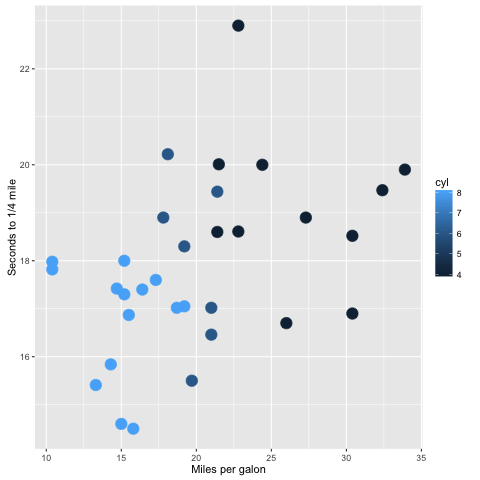
\includegraphics[width=10cm]{fig/plot1} % not necessary to give extension - now you can shift between compiling to ps or to pdf without any problems
 
\caption[Do not end short caption with full-stop]{Each figure must be supplied with a long caption, making the figure stand-alone and ended with a full-stop.}

\end{figure}





\newpage





% SUBFIG EXAMPLE
%================
%
% usage: \subfloat[][caption]{...figure code...\label{label}}

The subfigures are Figures \subref{firstfigure}, \subref{secondfigure}, \subref{thirdfigure} and \subref{fourthfigure}.

\begin{figure}
\centering

\subfloat[][First subcaption (No full-stop)]{
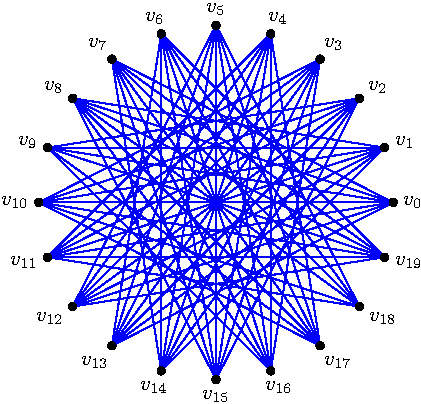
\includegraphics{fig/figure}
\label{firstfigure}
}
\quad
\subfloat[][Second subcaption (No full-stop)]{
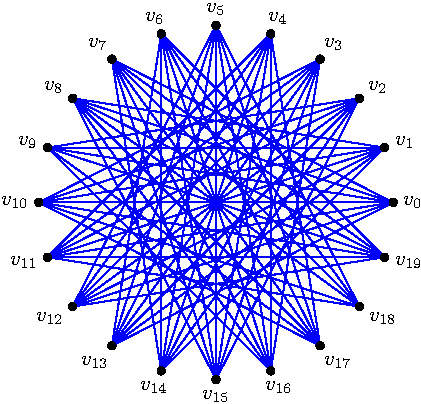
\includegraphics{fig/figure}
\label{secondfigure}
}
\\
\subfloat[][Third subcaption (No full-stop)]{
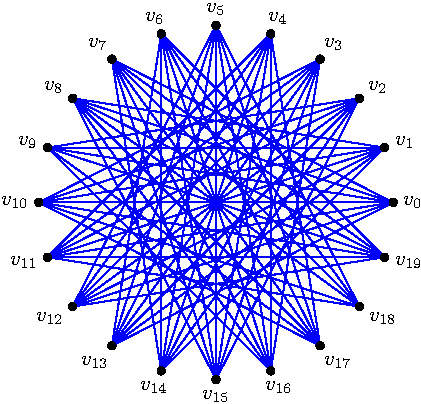
\includegraphics{fig/figure}
\label{thirdfigure}
}
\quad
\subfloat[][Fourth subcaption (No full-stop)]{
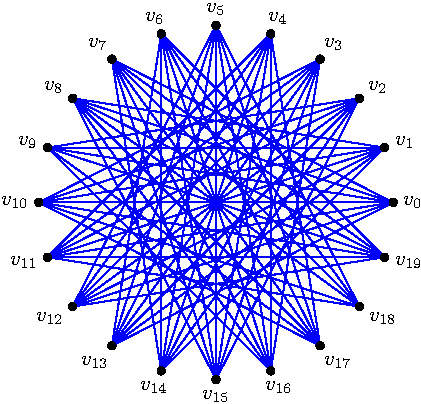
\includegraphics{fig/figure}
\label{fourthfigure}
}
\caption[Do not end short caption with full-stop]{End the main caption with a full-stop, but not each of the sub-figure captions!}
\label{thislabel}
\end{figure}
            % remove if NA
%%%%%%%%%%%%%%%%%%%%%%%%%%%%%%%%%%%%%%%%%%%%%%%%%
%
% how to typeset algorithms
%
%%%%%%%%%%%%%%%%%%%%%%%%%%%%%%%%%%%%%%%%%%%%%%%%
\chapter{Algorithms}

% USE THE TEMPLATE BELOW FOR YOUR ALGORITHMS
%============================================
%
% \begin{algorithm}
% 
% \SetKwInOut{Input}{Input}
% \SetKwInOut{Output}{Output}
% 
% \Indm
% \Input{Description of the input to the algorithm.}
% \Output{Description of the output from the algorithm.}
% \Indp
% 
% \BlankLine
% 
%   % main algorithm code here
% 
% \caption{Algorithm example}
% \label{alg}
%
% \end{algorithm}



\begin{algorithm}

\SetKwInOut{Input}{Input}
\SetKwInOut{Output}{Output}

\SetKwData{Left}{left}
\SetKwData{This}{this}
\SetKwData{Up}{up}
\SetKwFunction{Union}{Union}
\SetKwFunction{FindCompress}{FindCompress}

\Indm
\Input{Description of the input to the algorithm.}
\Output{Description of the output from the algorithm.}
\Indp

\BlankLine

\emph{special treatment of the first line}\;
\For{$i\leftarrow 2$ \KwTo $l$}{
  \emph{special treatment of the first element of line $i$}\;
  \For{$j\leftarrow 2$ \KwTo $w$}{\label{forins}
    \Left$\leftarrow$ \FindCompress{$Im[i,j-1]$}\;
    \Up$\leftarrow$ \FindCompress{$Im[i-1,]$}\;
    \This$\leftarrow$ \FindCompress{$Im[i,j]$}\;
    \If{\Left compatible with \This}{\label{lt}
      \lIf{\Left $<$ \This}{\Union{\Left,\This}}\;
      \lElse{\Union{\This,\Left}\;}
    }
    \If{\Up compatible with \This}{\label{ut}
      \lIf{\Up $<$ \This}{\Union{\Up,\This}}\;
      \lElse{\Union{\This,\Up}}
    }
  }
  \lForEach{element $e$ of the line $i$}{\FindCompress{p}}
}

\caption[Do not end short caption with full-stop]{Algorithm example}
\label{alg}

\end{algorithm}




\begin{algorithm}[t]
%\SetAlgoNoLine
 \Input{A tree $T$ represented by an array {\sf Parent}$[1,\ldots,n]$.}
\Output{A minimum secure dominating set of $T$, represented by a boolean array $X$.}
\For{$i\leftarrow 1$ to $n$}{
{\sf A3Label}$[i] \leftarrow$ {\sc False}\;
$X[i] \leftarrow$ {\sc False}\;
{\sf Labels}$[i] \leftarrow [0,0,0,0,0,0,0]$\;
{\bf if} vertex $i$ is a anchor of $T$ {\bf then} {\sf Branch}$[i] \leftarrow$ {\sc True}\;
{\sf Previous1Label}$[i] \leftarrow 0$\;
}
\For{$i\leftarrow n$ down to $2$}{
$\ell \leftarrow$ {\sf\bf EffectiveLabel}({\sf Labels}[$i$])\;
{\bf if} $\ell$ is odd {\bf then} $X[i] \leftarrow ${\sc True}\;
{\sf Labels$[$Parent$[i],\ell(i)+1 \ (\rm{mod}\ 7)]$} $++$\;
\If{$\ell=2$ {\bf and} {\sf Branch$[$Parent$[i]]$}}{
{\sf A3Label[Parent}$[i]] \leftarrow$ {\sc True}\;
{\sf prev} $\leftarrow$ {\sf Previous1Label$[$Parent$[i]]$}\;
{\bf if} {\sf prev} $>0$ {\bf then} $X[${\sf prev}$] \leftarrow$ {\sc True}\;
}
\If{$\ell=0$ {\bf and} {\sf Branch$[$Parent$[i]]$}}{
\If{{\sf A3Label$[$Parent$[i]]$}}{
$X[i] \leftarrow$ {\sc True}\;
}
\Else{
{\sf prev} $\leftarrow$ {\sf Previous1Label$[$Parent$[i]]$}\;
{\bf if} {\sf prev} $>0$ {\bf then} $X[${\sf prev}$] \leftarrow$ {\sc True}\;
{\sf Previous1Label$[$Parent$[i]] \leftarrow i$}\;
}
}
}
$\ell \leftarrow$ {\sf\bf EffectiveLabel}({\sf Labels}[$1$])\;
{\bf if} $\ell$ is odd {\bf then} $X[1] \leftarrow ${\sc True}\;
{\bf if}  {\sf Labels}$[1,j]=0$ for $j=1,3,4,5,6$ {\bf then} $X[1] \leftarrow$ {\sc True}\;
{\bf if} {\sf Labels}$[1,j]=0$ for $j=1,3,5,6$ {\bf and} {\sf Labels}$[1,0] \geq |${\sf Labels}$[1]-1|$  {\bf then} $X[1] \leftarrow$ {\sc True}\;
\If{$\ell=3$}{
{\sf prev} $\leftarrow$ {\sf Previous1Label$[1]$}\;
{\bf if} {\sf prev} $ > 0$ {\bf then} $X[$\sf{prev}$]$ $\leftarrow$ {\sc True}\;
}
\Return[$X$]\;
\caption[{{Do not end short caption with full-stop}}]{{\sf\bf DefendTree}}
\label{Alg:Tree}
\end{algorithm}

         % remove if NA


%=================================================
% include your chapters here
%=================================================
\chapter{Introduction} \label{ch1_heading}
% put these two lines after every \chapter{} command

\startarabicpagenumbering % must be just after the first \chapter{} command

%%%%%%%%%%%%%%%%%%%%%%%%%%%%%%%%%%%%%%%%
%%%%% Actual start of Introduction %%%%%
%%%%%%%%%%%%%%%%%%%%%%%%%%%%%%%%%%%%%%%%

With increasingly sophisticated financial industries, so too has the nature of financial crime become more sophisticated. Over the years, financial institutions could construct and combine different processes and technologies that would help combat financial crime. However, by integrating these critical infrastructure elements, financial intuitions are still incapable of entirely grasping the complexity of financial crime. Therefore, financial crime remains a serious complication. A survey conducted in 2018 estimated that the total turnover losses due to financial crime (from the 2373 counties surveyed worldwide) are USD\ 1.45 trillion. More specifically, it is estimated that the total turnover losses due to money laundering are USD\ 267 billion \citep*{begolli2019revealing}. These statistics are astounding, however, financial losses are only one of the consequences of financial crime. Money laundering has several other economic consequences, such as undermining the legitimate private sector and the integrity of financial markets, loss of economic policy, economic distortion and instability, etc. In addition, the social consequences of money laundering are that they financially support crimes such as drug and human trafficking. Therefore, criminals gain the opportunity to expand their operations and adversely impact society \citep*{mcdowell2001consequences}. 

Much has already been done to try and combat the issue of money laundering. \textit{Anti-money laundering} refers to the procedures, laws, and regulations intended to prevent criminals from secretly obtaining illegal funds as a source of legitimate income \citep*{kenton_2021}. Banks are obligated to comply with anti-money laundering regulations. These anti-money laundering compliance programs are enforced due to banks being at high risk to money laundering and other financial crimes \citep*{sanctionscanner}. Therefore, banks specifically design anti-money laundering processes to detect and prevent money laundering. 

In the past few decades, rule-based approaches have been prevalent among banks in dealing with money laundering \citep*{chen2018machine}. These rule-based approaches can either be human-driven or machine-driven. The human or machine-driven mechanisms strive toward one common goal - using client data (historical, transactional, personal, etc.) to develop rules that govern criminals' behaviour. The idea behind a rule-based model is that based on certain transaction scenarios, rules are developed. For the human-driven rule-based approach, domain experts or consultants develop these rules. As the name implies, the machine-driven rule-based approach is when some algorithm does the rule extraction. The rules developed are applied to daily transactions and notify the bank when certain transactions are suspicious. The set of rules is updated if any nuances are identified. Generally, human-driven rule-based approaches are not sufficient to detect financial crimes due to the dynamic nature of criminals, the high volume of data,  and the variety of data that needs to be processed \citep{chen2018machine}. Machine driven rule-based approaches are much more effective in processing huge amounts of financial data. However, the majority of the vanilla rule-based algorithms do not deliver good predictive performance when the rules are applied to new instances. More recently, financial institutions adopted \textit{machine learning} approaches to aid this shortcoming of rule-based approaches. Machine learning is very powerful since it exploits the possibilities of finding an empirical solution to a problem that does not have an analytical solution by using the available data. Therefore, machine learning approaches have the ability to detect complex non-linear patterns in data. Although banks heavily rely on rule-based systems (human and machine-driven) to filter out suspicious transactions, they are partnering with researchers to venture into the feasibility and practicality of implementing machine learning techniques to aid their anti-money laundering processes \citep{chen2018machine}. Examples of machine learning and data mining techniques that have already been applied in a banking context to detect suspicious transactions are outlier detection, support vector machines (SVM), fuzzy logic, clustering, neural networks, genetic algorithms, Bayesian networks, and sequence matching \citep*{al2021financial,abdallah2016fraud, ngai2011application, gao2007framework}. The predominant approach to implementing these techniques consists of using historical transactional data and client-related data to build statistical models that provide a degree of risk of criminal activity. 

\citet*{baesens2015fraud} mentions that networks or graphs give us the ability to map relationships that exists in the real world. For example, if a client makes occasional payments of high amounts to another banking client in a banking context, one might infer some relationship between the two clients. This project will investigate an unconventional approach to help classify the risk of a banking client being involved in any money laundering activity. The project will use complex network analysis and graph theory concepts to extract \textit{network features} or \textit{metric}s from financial data to serve as input to a statistical model. In short, network features describe characteristics of a network or graph's elements (vertices and edges). Also, they  can be the features describing the characteristics of a network as a whole.  Standard machine learning approaches deployed in most anti-money laundering processes do not include network metrics as part of machine learning models inputs. The project aims to establish evidence suggesting that incorporating network metrics in the learning process can be advantageous for conventional anti-money laundering approaches. 

The project will incorporate network metrics to try and capture the relational aspects between banking clients. This relational and other relevant information is provided to a machine learning model as input. Therefore, the network analytic's will function as a feature engineering step.  Emphasis is placed on feature engineering and not data pre-processing.  Although the paper will implement feature engineering and data pre-processing, they represent two different steps. \textit{Feature engineering} is the process of creating features from the data, and \textit{data pre-processing} is the process of altering the data such that it is in a more suitable form for downstream modelling applications \citep*{brownlee_2021, patidar_2021}. Organised crime is a social phenomenon and has a strong relational component attached to it \citep{baesens2015fraud}. Therefore, the project's hypothesis, or premise, is that incorporating these relational components as additional features could improve prediction accuracy, robustness, or both of the machine learning detection models. Figure \ref{fig:ch1_project_framework} illustrates, on a high level, the implementation process of the project. The project has 4 phases (numbered 1-4). The project's first phase generates the raw data (using the AMLSim simulator). Two data sets are primarily used from the simulator's output - the transactional data set and the accounts data set. A pivotal sub-phase is performed upon transitioning from the first phase to the second phase. This sub-phase is the \textit{feature engineering process}. The feature engineering sub-phase generates three structured data tables - \textit{network feature} data table, \textit{transactional feature} data table, and \textit{combined feature} data table. The third phase of the project is the modelling phase which involves the data pre-processing of the structured data, defining the model's architecture, tuning the model hyper-parameters, training the model, and evaluating the model's performance. The results interpretation is the final phase of the project. This phase is concerned with documenting the findings of the project. A more detailed explanation each phase is provided in Chapter \ref{ch3_heading}.   

Many financial crimes exist within a bank, such as credit card fraud, transactional fraud, online banking fraud, etc. However, the project will specifically focus on \textit{money laundering}. The project aims to provide evidence that network metrics/features can improve the performance of machine learning based anti-money laundering processes and essentially aid in the risk profiling of banking clients. The project will investigate how the performance of various classification models are influenced when the inputs to the models consist of i) network features, ii) transactional features,  and iii) network and transactional (combined) features. In short, transactional features are standard features banks use in their risk profiling processes. Also, the data used in the project is synthetically generated using \textit{AMLSim} - a financial transaction simulator developed for research in improving anti-money laundering processes \citep*{AMLSim} . More of the data and how it is generated is mentioned in section \ref{ch3_sub_heading_data}. 

To adequately execute what the project proposes, the following question needs to be considered: 
\begin{center}
\textit{Using historical client transactional data, how can one obtain sufficient evidence that suggests that including network/graph features as inputs to a classification model can improve the classifier's performance in identifying if a banking client is involved in any money laundering activity?}    
\end{center} 

The methodologies used to answer the above question included complex network theory and machine learning. Complex network analysis was used to construct a client network structure and extract network information that gives insight into a client's position and influence ability. On the other hand, the project used machine learning to identify hidden patterns within the data. The thinking behind incorporating the two methodologies was that the network analytics would act as a feature engineering step, generating valuable features for the machine learning model. According to the project's hypothesis, the feature engineering step would ensure that the machine learning model will produce more accurate predictions.  

An outline of the paper is as follows, Chapter \ref{ch2_heading} provides a comprehensive review on the core elements of the project - money laundering, complex network analysis, and machine learning. Next, chapter \ref{ch3_heading} explains the methodology of the project. This chapter is divided into three subsections, explaining sequentially how the data is generated, transformed, and used as input to different classification models. Chapter \ref{ch3_heading} concludes by illustrating the results of the project. Finally, chapter \ref{ch4_heading} discusses the findings of the project as well as recommendations for future work.         

% FCH1_1 - Project framework
\begin{figure}
	\begin{center}
		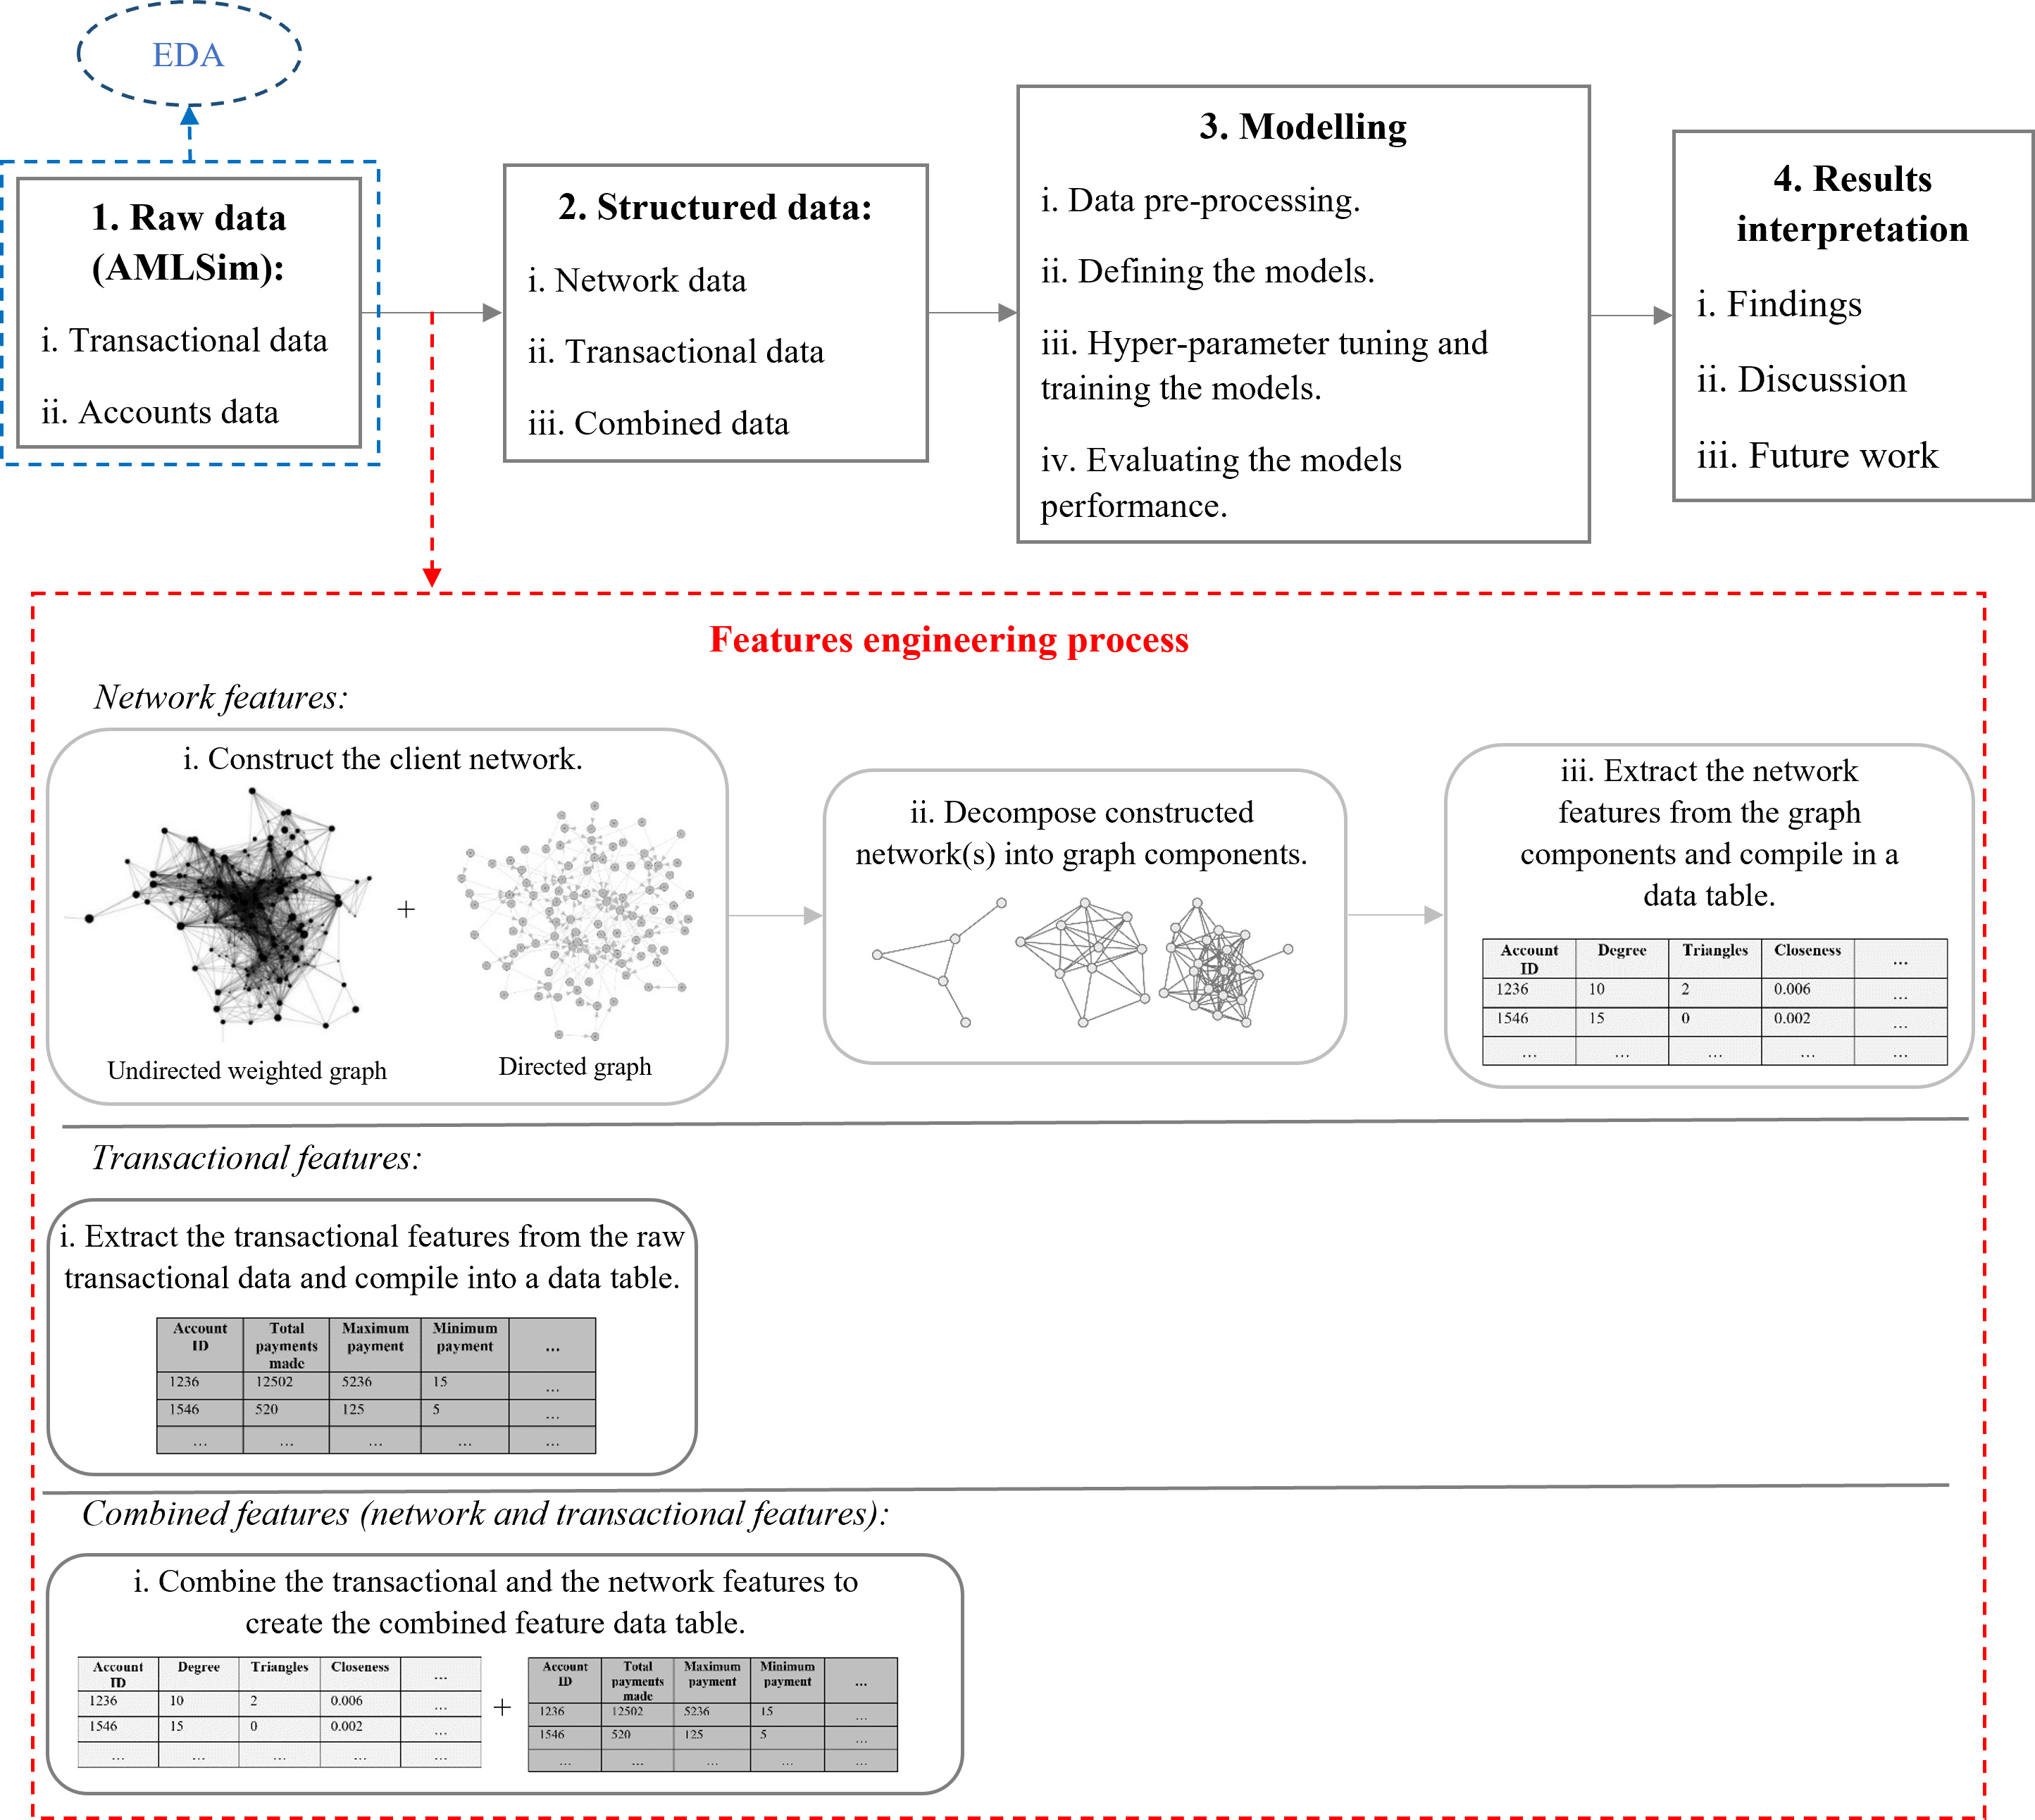
\includegraphics[scale=0.75]{fig/CH1/proposed_project_framework.png}
		\caption{The high-level overview of the implementation of the project. The project has 4 phases (numbered 1-4). The project's first phase generates the raw data (using the AMLSim simulator). The feature engineering process is a sub-phase (between phases one and two) that generates three structured data sets. First, the network feature data table is generated by constructing an undirected weighted network and a directed network. Both networks are constructed from the transactional and accounts raw data (the edges representing the transactions and the vertices the banking accounts). After the networks are constructed, the graph components are extracted. Then, the network features are derived from each component and assigned to each bank account. The second data table is populated by extracting common transactional features for each bank account using the raw transactional information. Lastly, the third data table combines the network feature data table and the transactional feature data table. The third phase of the project is the modelling phase. This phase consists of the modelling procedure implemented in the project. The last phase of the project, the results interpretation phase, is concerned with the project's findings.}
		\label{fig:ch1_project_framework}
	\end{center}	
\end{figure}


%%%%%%%%%%%%%%%%%%%%%%%%%%%%%%%%%%%%%%%%%%%%%%%%
%
% start writing
%
%%%%%%%%%%%%%%%%%%%%%%%%%%%%%%%%%%%%%%%%%%%%%%%%

%%%%%%%%%%%%%%%%%%%%%%%%%%%%%%%%%%%%%%%%%%%%%%%%
%
% start writing
%
%%%%%%%%%%%%%%%%%%%%%%%%%%%%%%%%%%%%%%%%%%%%%%%%


\chapter{Literature study} \label{ch2_heading}

%\textbf{[Chapter introduction and context]}

To adequately answer the projects research question and test its hypothesis, a comprehensive understanding of the following topics needs to be established: i) Money laundering, ii) Complex network analysis for anti-money laundering processes, and iii) Machine learning approaches applied to an anti-money laundering context. Therefore, the chapter aims to give necessary background information on the topics mentioned earlier and investigate research that has already been conducted in these fields.        
\section{Financial crime - Money Laundering}

It is essential to understand money laundering and its known forms before thinking of how anti-money laundering processes can be improved. In short, money laundering is the process of making money that has been generated through illegal or criminal activities seem legitimate by misleading that the money launderer obtained the money in legitimate ways \citep*{buchanan2004money}.  \citet*{mcdowell2001senior} explained that the money laundering process contains three steps:

\begin{enumerate}

\item \textit{Placement}:  The process of placing illegal funds into financial institutions through wire transfers, deposits, or alternative means. 

\item \textit{Layering}: The process of separating the funds by performing a series of financial transactions that obscure the funds' origin.    

\item \textit{Integration}: The process of reintegrating the funds with formal sector economic activity. 

\end{enumerate}    

\citet{buchanan2004money} explained similar steps regarding the money laundering process. However, she provided additional information: The laundering mechanism is most vulnerable during the placement step because usually, money generated from unlawful activities takes the form of paper money, which is often difficult to conceal in large amounts. Therefore, money launderers carefully need to establish ways to introduce large amounts of cash into the financial system incrementally. Money launderers commonly use front corporations to deposit cash or cashing businesses to convert cash to financial instruments such as money orders, traveller's checks, and cashier checks. The layering step aims to construct a complex web of transactions representing legitimate financial activity based on the transactions' volume, frequency, and monetary value. If the layering is complete, it is challenging to reconstruct a paper trail. Also, offshore financial institutions play an essential role in the layering step. Finally, regarding the integration step, standard financial instruments used to reintegrate the ``washed'' funds are bills of lading and guarantees, banknotes, bonds, and letters of credit.   	      

The essence of the money laundering process is encapsulated within the steps mentioned above. However, these steps are executed using different money laundering tools and techniques. For example, \citet{buchanan2004money} explained that there are seven tools or techniques most commonly used by money laundered that help them successfully launder money. These techniques are:

\begin{enumerate}

\item \textit{Structuring}: A person is known as a ``smurf'' when they intentionally avoid reporting financial transaction requirements by making deposits that are less than the country's prescribed threshold. In South Africa, this threshold is defined in the FIC act that states that all institutions are obligated to report on cash transactions bigger than the prescribed threshold. According to the financial intelligence centre, the prescribed threshold limit in South Africa is R24 999,99 \citep*{fic2001}. Money launders deposit large amounts by breaking them up into increments less than the prescribed limit and depositing these increments from different accounts. As a result, money launderers avoid reporting the requirements of cash transactions to authorities. The prescribed threshold may vary from country to country. For example, the prescribed threshold in the US is \$10 000 \citep*{yale2021reporting}.        

\item \textit{Front companies}: Front companies are considered to be an effective money laundering tool for two reasons: i) front companies do not necessarily require the collaboration of financial institutions and, ii) detection of criminal activity within front companies that are conducting legitimate business is challenging (especially when the front company is exempt from any currency transaction reports). Businesses that commonly function as front companies are cash-rich, for example, liquor stores, restaurants, cheque cashing businesses, and travel agencies. Also, companies that import and export goods can function as front companies. These companies launder money by double invoicing, over/undervalued goods, inflating prices for imported goods, and financial exports.

\item \textit{Trade misinvoicing}: This is a widespread money laundering technique that involves the misinvoicing of international trade transfers. Trade misinvoicing involves illegally moving money across borders by deliberately falsifying the type of commodity, its volume, and its value in an international commercial transaction. For example, consider the scenario where criminals used company X, a precious metals front company, for trade misinvoicing. Company X can create falsified invoices for importing gold from Peru. As a result, illicit funds can be transferred to Peru. Trade invoicing is very dangerous since criminals can transfer substantial sums of money across international borders.  

\item \textit{Shell companies}: According to the Financial Action Task Force, a shell company is defined as an institution ``that does not conduct any commercial or manufacturing business or any other form of commercial operation in the country where their registered office is located.'' Shell companies are often established in countries where offshore financial centres are characterised by: no or low taxes based on business income/investment, looser tax codes, strong bank secrecy, and no need for the physical presence of financial institutions, corporate or legal entities within the jurisdiction in question. Examples of offshore financial centres are Panama, the Bahamas, the Cayman Islands, and the Netherlands. The volume of transactions and secrecy laws of the offshore financial centres make it nearly impossible to investigate potential money laundering instances.   

\item \textit{Correspondent banks}: Correspondent banking has recently raised severe money laundering concerns. Correspondent banks are banks situated in a country to provide services for another bank or financial institution in a foreign country. Figure \ref{fig:ch2_correspondent_bank} gives a visual illustration of the relationship between the banking clients, domestic banks, and correspondent banks and tries to convey the core idea of when money gets wired across different jurisdictions. The risk for the money laundering process arises due to differences in anti-money laundering compliance programs between the foreign and domestic banks (originator A's and beneficiary B's domestic banks, see Figure \ref{fig:ch2_correspondent_bank}). It is possible that a foreign bank's anti-money laundering compliance program is not sufficient to meet the anti-money laundering requirements of a domestic bank.

% FCH2_1 - Correspondent bank
\begin{figure}[h]
	\begin{center}
		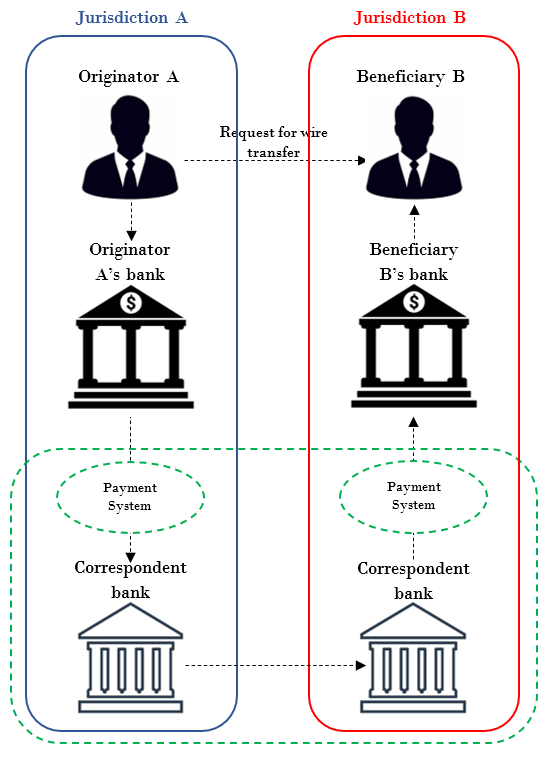
\includegraphics[width=8cm]{fig/CH2/correspondent_bank_01.png}
		\caption{The arrows dictate the flow of information between the entities in the diagram. The role of corresponding banks can be explained as follows. Originator A would want to wire transfer money to beneficiary B. Originator A will log this request with their domestic bank (acting as a responded bank). Originator A's bank will then log the transaction request with the correspondent bank. As a result, the correspondent bank, which has both jurisdictions, can transfer the funds to beneficiary B's domestic bank. Beneficiary B's domestic bank (also acting as a respondent bank) will then make the funds available to beneficiary B.}
		\label{fig:ch2_correspondent_bank}
	\end{center}	
\end{figure}
   
\item \textit{Mirror trading}: The non-fraudulent meaning of mirror trading is when a forex or stock trader mimics the trading strategy of experienced brokers \citep*{chen_2021}. The recent incident with Deutchbank in 2017 obscured the meaning of mirror trading.  The fraudulent meaning of mirror trading is when an individual that owns two accounts buys contracts for one account while selling an equal amount of contracts from the other. The incident with Deutsch bank will be used as a motivating example. A Russian customer of Deutsch bank bought securities against ``Russian Ruble'' from Deutsch bank in Moscow. Simultaneously, a non-Russian customer of Deutsch bank sold the same number of securities to Deutsch bank in London in exchange for US dollars. Unfortunately, Deutsch bank failed to connect the two customers working together at this scheme. As a result, mirror trading (the fraudulent type) was used as a tool to move funds (Russian Ruble) out of Russia and into other jurisdictions and currencies (US dollar). 

\item \textit{Parallel banking systems}: There is a possibility that illicit funds never enter mainstream financial systems. Instead, criminals use underground banking systems (parallel banking systems) to launder money. Examples of parallel banking systems are Hawala and Hundi systems in India or the Chop or fei chi in China. The basic idea behind these parallel banking systems are as follows: i) a person can deposit money in exchange for some marked object (chip, ticket, etc.) which is impossible to replicate; ii) a person can exchange the object for its monetary value in another country (in paper cash); iii) upon exchange, the person pays a commission fee (typically 5-15 percent of the original amount). The exact functioning of these parallel banking systems is unknown. Experts say that these systems can range from being extremely complex to being very simplistic \citep*{schramm2003evolution}. These parallel banking systems are ideal for money launderers since there is little or no documentation about the events, and no funds will cross borders. The challenge for regulatory authorities is to be vigilant for indications that suggest that parallel banking systems are present. 
\end{enumerate}

Now that a preliminary understanding of the problem - money laundering and its components have been established, the paper can shift its focus towards the solution - anti-money laundering. As mentioned in the introduction of the paper, anti-money laundering refers to the regulations, procedures, and laws intended to prevent criminals from obtaining legitimate funds generated by illicit activities. The history of anti-money laundering dates back to the 1970s when legislation started to develop. In 1989 the fight against money laundering intensified with establishing the Financial Action Task Force (FATF). The FATF resulted from a group of countries that came together to investigate and construct anti-money laundering measures, establish international anti-money laundering standards, and promote adequate implementation thereof. Various anti-money laundering regulations are imposed on financial institutions due to their vulnerability to the crime. Therefore, anti-money laundering legislation and regulations ensure that financial institutions have adequate anti-money laundering processes. 

\citet*{sudjianto2010statistical} provided an overview of a general anti-money laundering process, see Figure \ref{fig:ch2_aml_process}. The first phase of anti-money laundering is the customer screening phase. This phase evolves, enforcing the \textit{Know Your Customer Policy} and implementing an \textit{Enhanced Due Diligence} check during the account opening process. The Know Your Customer Policy is a set of standards used by financial institutions to verify customers personal profiles, risk profiles and financial profiles. The Enhanced Due Diligence check is primarily done to check the customer's identity. The information gathered from the Know your Customer and Enhanced Due Diligence check is processed by a risk rating model (an inference model or rule-based model) to output a risk score, which indicates the potential customer's risk. The second phase of the anti-money laundering process continuously monitors customer transaction activity. \citet{sudjianto2010statistical} explains that there are four steps in the customer transaction monitoring phase:

\begin{enumerate}
    \item \textit{Identify:} The focus of this step is to identify suspicious activity. The step entails observing if historically known suspicious activity occurs, surveillance of high-risk customers (identified in the first phase), and trying to detect emergent patterns that might indicate risky behaviour.     
    
    \item \textit{Prioritise:} The first step could generate false positives cases. Therefore, the goal of the prioritise step is to prioritise and rank cases that fraud experts should investigate later on.
    
    \item \textit{Investigate:} After prioritising suspicious cases, experts investigate these cases. The investigation requires intense human resource capacity and manual intervention, unlike the previous two steps. It is up to the expert to investigate and pull information from various sources to ``create a story'' for their investigation.    
    
    \item \textit{Report:} If a case is deemed suspicious, it needs to be reported for further investigation by law enforcement. A detailed report is needed for authorities to continue the investigation and promote learning. In addition, banking personal must make system updates to identify future cases with similar characteristics.    
    
\end{enumerate}

% FCH2_2 - AML process
\begin{figure}[h]
	\begin{center}
		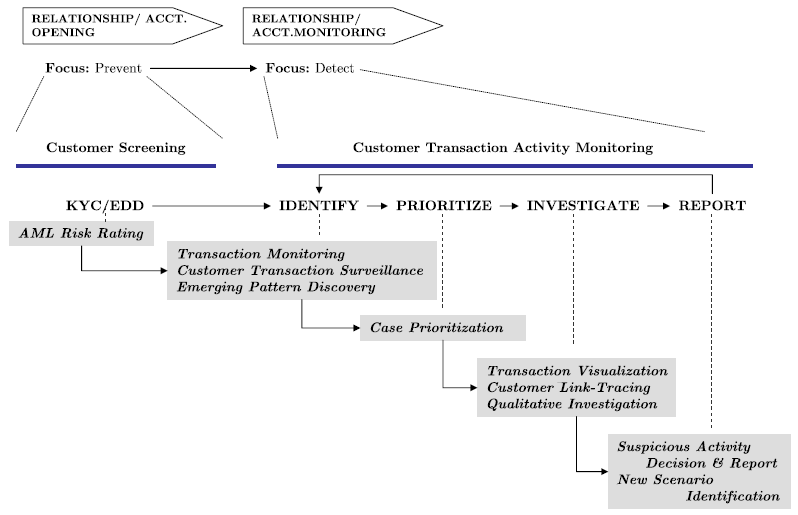
\includegraphics[scale=0.75]{fig/CH2/aml_process_02.png}
		\caption{The general anti-money laundering process as described by \citet{sudjianto2010statistical}. The process consists of two phases, customer screening and customer transaction activity monitoring. The first phase enforces the Know Your Customer (KYC) policy and performs an Enhanced Due Diligence check (EDD). The second phase consists of four steps, i) identify, ii) Prioritise, iii) Investigate, and iv) Report.}
		\label{fig:ch2_aml_process}
	\end{center}	
\end{figure}

There are multiple stages and steps within the anti-money laundering process. The project will not attempt to improve the entire process. However, the project will attempt to provide evidence that might improve a subset of the process, specifically identifying and prioritising steps within the second phase of the anti-money laundering process. For example, in generating the network features, the project will use historical transactions (obtained by the customer transaction monitoring phase) to construct a client network. The network features with other useful client features are then presented to some learning algorithm that seeks to \textit{identify hidden patterns} (step 1, phase 2 of the general anti-money laundering process) within the data. After choosing the best-suited learning algorithm, a model is constructed, which provides  the probability that a banking client is engaged in money laundering activities. Therefore, high-risk clients can be \textit{prioritised} (step 2, phase 2 of the general anti-money laundering process) by ranking each client based on their obtained risk score.   

It would be interesting to understand how the identification and prioritisation steps (Figure \ref{fig:ch2_aml_process}) are executed by different banks. Unfortunately, the literature vaguely explains the details of current industry-standard anti-money laundering processes, specifically those geared towards identifying suspicious transactions/clients and their ranking. This information gap is understandable because financial institutions prohibit publications since they contain sensitive content. However, literature seems to indicate that most banks implement a rule-based approach in identifying suspicious transactions \citep{abdallah2016fraud, chen2018machine, sudjianto2010statistical, gao2007framework}. Unfortunately, the degree of complexity of the rule-based approaches is not mentioned. However, there is a consensus that rule-based approaches are predominantly implemented due to their ability to effectively filter through masses of client transactions.   

On the other hand, rule-based systems implemented in commercial banks experience the problem of not adapting their rules quickly enough to capture the dynamic behaviour of money laundering criminals. Trying to capture the dynamic behaviour of money laundering criminals is only one of the challenges the modern-day fraud detection systems need to handle. Literature details various challenges and issues that general fraud detection systems face \citep{abdallah2016fraud, sudjianto2010statistical, gao2007framework, van2017gotcha} . These challenges apply to banking fraud (credit card fraud and money laundering) and other fraud areas such as insurance fraud, telecommunication fraud, online fraud, etc.    

From the papers investigated, \citet{abdallah2016fraud} defined the most comprehensive set of challenges and issues that modern-day fraud detection systems encounter. These challenges are i) Concept drift, ii) Skewed class distributions, iii) Large amounts of data, and iv) Infrastructure for real-time detection. \textit{Concept drift} is described as a phenomenon in that the underlying model (or concept) changes over time \citep*{abbass2004online}. This phenomenon directly relates to the \textit{drift phenomenon concept}, described in the context of fraud detection systems, when the behaviour of fraudsters and legitimate users continuously changes \citep*{gama2014survey}. Concept drift is a tremendous challenge when statistical learning models are constructed since there is a possibility that the model is constructed using outdated data. Using outdated data is problematic because of the high likelihood that the relationship between variables considered in the model has already changed \citep{gama2014survey}. The second challenge mentioned by \citet{abdallah2016fraud} is \textit{skewed class distributions} or imbalanced classes. In fraud detection systems, skewed distributions are when the typical instances (for example, legitimate transactions) exceed the amount known fraudulent instances (for example, suspicious transactions) by a significant factor \citep*{maes2002credit}. Skewed class distributions, especially when the variable of interest is in the minority class, can cause problems with the learning algorithm (assuming that the detection system uses one). If there is not enough data for the learning algorithm, it will not discover patterns within the data \citep*{abu2012learning}. The third challenge fraud detection systems experience is with the \textit{quantity of data}. Often vast amounts of data need to be processed by fraud detection systems. The data introduced to fraud detection systems have high dimensionality, meaning that the data set contains multiple features/variables/inputs/attributes.  The colossal size of the data sets makes it difficult for fraud detection systems to process this information and, secondly, in a timely manner. The final challenge mentioned by \citet{abdallah2016fraud} is that fraud detection systems are challenged with \textit{supporting real-time detection}. Therefore, these detection systems should be designed to efficiently use their resources (time and memory) to detect illicit activity immediately.

The challenges mentioned by \citet*{van2017gotcha}, \citet{sudjianto2010statistical}, and \citet{gao2007framework} had some overlap with the above-mentioned challenges. However, they did have the following to add: \citet{van2017gotcha} added that fraud has the characteristic of being \textit{imperceptibly concealed}. In fraud detection systems, the term means that criminals expertly disguise themselves as honest clients in all possible areas (including the data). Therefore, defining what makes a client or transaction honest is the true challenge for any fraud detection system. \citet{sudjianto2010statistical} also added that in the case of a fraud detection system that utilises a statistical model, the problem of \textit{learning mislabeled classes} could arise. This problem occurs particularly with money laundering because most suspicious cases (reported by the anti-money laundering process) are evaluated externally. The result of these investigations are often not promising, and the financial institution rarely learns anything. Therefore, suspicious cases are easily mislabeled.

Providing a solution for each of the challenges mentioned above is beyond the project's scope. However, as mentioned in the introduction of the project, the project's objective is to provide evidence that incorporating network features into the feature set used as input to a machine learning model will enhance the performance of the  money laundering classifiers. Therefore, it is beneficial for the project to be aware of the challenges mentioned above and their mitigation strategies. The following section gives an overview of machine learning, a brief discussion of popular machine learning algorithms used in anti-money laundering processes, and examples of how machine learning is applied in an anti-money laundering context.  

\section{Machine learning approaches for financial fraud detection}.

\citet{abu2012learning} explains that there exist various views of what ``learning from data'' is. \textit{Statistics} is one of the fields that offers its view on the task. More specifically, statistics is concerned with probability theory and applying said probability theory in building \textit{models} which replicate the underlying data generating process. The statistician is thus conscious of the structure proposed for the underlying process and interprets at the hand of that structure. Another view of learning from data is the view presented by the \textit{data mining} discipline. Data mining is described as a practical field that focuses on finding anomalies, patterns, or correlations in large relational databases. Although the field of machine learning contains components of both these fields, it should be distinguished as a learning view on its own.
 
The field of machine learning is the main field dedicated to learning from data \citep{abu2012learning}. The basic premise of learning from data from machine learning's view is to utilise a set of observations to undercover underlying processes. This is a very broad premise, and although the premise is somewhat shared with statistics, the main difference  between machine learning and statistics lies in their approach. Machine learning is only concerned with \textit{predicting} what is generated by the underlying process and not establishing the underlying data generating process (as in statistics). For these purposes, machine learning relies on over-specified mathematical structures, for which the mappings are not easily interpretable, and careful application of probability theory in identifying a constrained configuration of said structure is useful for predicting observations. This being said, there are similarities between how both are applied. For example, both rely heavily on probability theory and mathematical models. Statistics results in more interpretable propositions for the relationship between inputs and outputs, whilst machine learning sometimes provides improved prediction performance at the cost of interpretability. Both the qualitative and quantitative objectives of the study dictate how useful and appropriate either may be. The judgment in this regard is at the discretion of the analyst. This project will use machine learning as one of the main components in (dis)proving its premise. 

From machine learning's view, it is difficult to encapsulate the broad premise of learning from data within a single framework. Therefore, as a result, different learning paradigms were developed to deal with the different situations and assumptions. The following basic notation needs to be established before listing and describing the different learning paradigms or types of learning. This notation was predominantly adopted from \citet{abu2012learning} and \citet*{et2020pien}.
 
A data set $\mathcal{D}$ contains $N$ observations each consisting of a response, denoted by $y_i$, and vector of features/predictors associated with the response variable denoted as $\{\boldsymbol{x}_i = [x_{i1},x_{i2},\ldots, x_{ip}]^T :i = 1,2,\ldots,N$\}. In the case where the response is \textit{multi-valued} then it will be denoted by $\{\boldsymbol{y}_i = [y_{i1},y_{i2},\ldots, y_{iq}]^T :i = 1,2,\ldots,N\}$, where $p$ and $q$ denote the input and output dimensions respectively. Furthermore, $f$ will denote a unknown target function, which describes the relationship between all possible input values (input space), denoted by $\mathcal{X}$, and their corresponding responses (output space), denoted by $\mathcal{Y}$. 

Now that the paper established the preliminary notation, it can further investigate the different learning paradigms. The two most popular learning paradigms or types of learning are \citep{abu2012learning,et2020pien, james2013introduction}:

\begin{enumerate}
    \item \textit{Supervised learning}: A supervised learning task aims to predict some response. This task involves using models and learning algorithms to extract a pattern from the data (i.e. finding a relationship between the predictors and responses). For example, suppose we have the predictors, $\boldsymbol{x}_i$ and their associate response, ${y}_i$. With a supervised learning task, the goal is to find a function that best represents $f$. As a result, responses can be predicted (given the predictors), and an understanding of the relationship between the response and predictor variables (inference) is established.  The process of approximating $f$ is referred to as training the model. This process is possible due to the learning methods ability to ``supervise'' its performance, hence, why the task is called ``supervised learning''.
    
    \item \textit{Unsupervised learning:} In contrast to supervised learning, unsupervised learning tasks are strategies for identifying structures in the data without the aid of a response variable. Therefore, for every observation $i$, we have a vector of measurement $\boldsymbol{x}_i$ but no associate response $y_i$. Therefore, the learning type is called ``unsupervised'' due to the absence of the response variable that acts as a supervised mechanism. Unsupervised methods aim to discover the relationship between variables or between the observations.
    
\end{enumerate}

The learning paradigms mentioned above are not the only learning types. Other types of learning include reinforcement learning, semi-supervised learning, self-supervised learning, multi-instance learning, etc. Although much research has been done in applying unsupervised methods in the financial fraud domain \citep*{al2021financial, salehi2017data, abdallah2016fraud} this project will focus on \textit{supervised learning} applied in an anti-money laundering context. 

There are two common types of supervised learning problems \textit{regression} and \textit{classification}. Regression is described as a supervised learning problem with a numeric or quantitative response and classification as a supervised learning problem with a categorical or qualitative response \citep*{james2013introduction}. The general formulation of supervised banking fraud problems (including money laundering) is formulated as a binary classification problem:

Given a data set ($\mathcal{D}$) with predictors $\{\boldsymbol{x}_i:i = 1,2,\ldots,N\}$ and response $\{y_i:i = 1,2,\ldots,N\}$, where:

$$y_i = \left \{\begin{array}{ll} 
 +1 &  \text{if observation is `fraudulent'},\\ 
-1 & \text{if observation is `non-fraudulent'. } 
\end{array} \right.$$

 let the chosen learning algorithm pick $g$, from the set of candidate formulas, known as the hypothesis set $\mathcal{H}$, such that $g$ approximates $f$ ($g \approx f: \mathcal{X} \rightarrow \mathcal{Y}$). 

The above formulation may be an over-simplification of how certain supervised banking fraud problems are formulated. However, it conveys the central idea of the problem setup. Also, most supervised banking fraud problems are formulated as classification problems \citep{al2021financial, abdallah2016fraud, salehi2017data}. Therefore, the project specifically focused on \textit{classification} applied in an anti-money laundering context.

\section{Network analytic's for fraud prevention} \label{ch2_sub_heading_network}

Networks are ubiquitous in nature. Physical networks such as highways, electric power grids, subway systems, etc., are easily identifiable, but \textit{abstract} networks are less tangible such as social relationships, biological systems, etc. Real-world networks, physical and abstract, generally are \textit{dynamic}. In short, dynamic networks are characterised by having entities that evolve over time \citep*{boccaletti2006complex}. For example, consider the case when we model the internet as a network with websites as its nodes and website links as the edges connecting these nodes. This network model is an example of a dynamic network model since the network topology will look differently at time step $t$ than at time step $t+1$. This is because users will probably add/remove certain websites and website links. Historically, the study of networks was predominantly a branch of discrete mathematics known as \textit{graph theory} \citep{boccaletti2006complex}. In 1736 the foundations of graph theory were established by Leonhard Euler. At the time, graph theory was very helpful in solving practical problems such as in a plumbing network, what is the maximum flow per unit time from source to sink, how to allocate $n$ jobs to $n$ people while maximising utility, etc. In the 1920s, principles of graph theory were later used to develop the study of \textit{social network analysis} (here, social network analysis does not reffed to analysing modern-day social networks but rather an approach for investigating social structures at the time). The study field arose due to the need to better understand relationships between social entities, whether attempting to model communication between members in a group, trades among nations, or economic transactions between corporations. More recently, a new field of network studies has become of interest to the academic community - \textit{complex network analysis}. \citet{boccaletti2006complex} defines complex networks as networks whose structures are irregular, complex and dynamically evolving in time. Complex networks analysis is commonly characterised by analysing networks containing thousands to millions of nodes and analysing the properties of the network that contain dynamical units \citep{boccaletti2006complex}. Most real-life networks are complex. \citet{boccaletti2006complex} defined graph theory as ``the natural framework for the exact mathematical treatment of complex networks'', and they stated that formally, a complex network is represented as a graph. Therefore, the application of graph theory will help extract the needed information from the projects complex network - the network of banking clients and their transactions.

Before discussing the different approaches on how the project can apply complex network analysis in an anti-money laundering context, the following definitions and notations need to be introduced, which describes a graph's type, topology (structure), size, and navigational properties. The notation was primarily adopted from  \citet{boccaletti2006complex}.

A graph $G$ can be either \textit{directed} or \textit{undirected}. A directed graph is where the \textit{links} (or lines, or edges) impose a direction or order between the \textit{network's nodes} (or points, or vertices). If there is no order or direction indicative in the network, then the graph is undirected. More formally if, $G = (\mathcal{N},\mathcal{L})$, where $\mathcal{N} = \{n_1,n_2,\ldots,n_N\}$ represents the set of nodes within graph $G$ and $\mathcal{L} = \{l_1,l_2,\ldots,l_K\}$ represents the set of links within graph $G$, then a undirected graph (directed graph) consist of two sets $\mathcal{N}$ and $\mathcal{L}$, such that $\mathcal{N} \neq \varnothing$ and $\mathcal{L}$ is a set of unordered (ordered) pairs of elements of $\mathcal{N}$. $N$ and $K$ represent the number of elements in $\mathcal{N}$ and  $\mathcal{L}$ respectively. From here on, the notation of $G(N,K) = (\mathcal{N},\mathcal{L})$ will be used if the nodes and links within a graph need to be illustrated (usually to emphasise the size of the graph). A specific node in the set $\mathcal{N}$ is usually referred to by its order $i$ in the set. In a undirected graph, $l_{ij}$ denotes the link between nodes $i$ and $j$. If a link is \textit{incident} in nodes $i$ and $j$, then it means that the link joins or connects the two nodes. In this case, nodes $i$ and $j$ are \textit{end nodes}. Also, if a link joins two nodes, they are referred to as \textit{adjacent} or \textit{neighbouring} nodes. The labelling of the links in a directed graph is defined differently due to the order being important. Therefore, a link in a directed graph is defined as $l_{ij}$,  where $l_{ij} \neq l_{ji}$. An illustration of how graphs are usually drawn can be seen in Figure \ref{fig:ch2_graph_types}. A way in which graphs are mathematically displayed is by using the \textit{adjacency} (or \textit{connectivity}) matrix $\bold{A}$. The adjacency matrix is a square matrix with the dimensions $N \times N$, where the entries of the matrix $\{a_{ij}:i,j = 1,\ldots,N\}$ represents a binary variable (typically 0 or 1) indicating if a link $l_{ij}$ exist between node $i$ and node $j$. For undirected graphs, the adjacency matrix is a symmetrical matrix with the diagonal of the matrix containing only zeros.    

A weighted network (such as graph (c) in Figure \ref{fig:ch2_graph_types}) is where each link in the network is given a numeric value that describes the strength of the connection between the end nodes. More formally, a weighted network is defined as $G^W = (\mathcal{N},\mathcal{L},\mathcal{W}_G)$, where $\mathcal{W}_G$ is the set of weights (or values) such that $\mathcal{W}_G = \{w^G_1,w^G_2,\ldots,w^G_K\}$. The matricial representation of $\mathcal{W}_G$ is matrix with dimensions $N \times N$, where the elements of this matrix, $w^G_{ij}$, indicates the weight value of the the link conncecting node $i$ and $j$. Typically, when $w^G_{ij} = 0$ nodes $i$ and $j$ is not connected and $w^G_{ii} = 0\: \forall \:i$. When referring to weighted networks, the paper will consider the case of positive symmetrical weights, meaning $w^G_{ij} = w^G_{ji} \geq 0; w^G_{ij} \in \mathbb{R}$.

The above standard definitions do not apply to \textit{multigraphs}. A graph is considered a  multigraph when \textit{loops} or \textit{multiple edges} are present. A loop is defined as a link between a node and itself. Multiple edges occur when two nodes are connected by more than one edge. The links in the cases mentioned above are referred to as \textit{self-edge} and \textit{multi-edge}, respectively \citep*{baesens2015fraud}.    

Regarding the size of graphs, the number of edges $K$, in graph $G$, is at most $N(N-1)/2$ (the case when all the nodes in the network is connected to each other - pairwise adjacent) and at least $0$. Also, a graph is said to be \textit{dense} if $K = \mathcal{O}(N^2)$ and \textit{sparse} if $K \ll N^2$. When considering a graph with  $K = \binom{N}{2} = N(N-1)/2$, then that graph is referred to as a \textit{complete} N-graph denoted by $K_N$. A common complete graph is a $K_3$ graph which is know as a \textit{triangle}. A triangle is a type of \textit{subgraph}. More formally, a subgraph $G^\prime = (\mathcal{N^\prime},\mathcal{L^\prime})$ of graph $G = (\mathcal{N},\mathcal{L})$ is a graph such that $\mathcal{N^\prime} \subseteq \mathcal{N}$ and $\mathcal{L^\prime} \subseteq \mathcal{L}$. If $\mathcal{G^\prime}$ possesses all the links of $G$ that joins two nodes in $\mathcal{N^\prime}$, then $\mathcal{G^\prime}$ is a subgraph \textit{induced} by $\mathcal{N^\prime}$ and is denoted as $\mathcal{G^\prime} = G[\mathcal{N^\prime}]$. If a subgraph is \textit{maximal} then it means that with respects to a certain property, the subgraph can not be futher extended without loosing that property. Finally, a subgraph constructed of the neighbourouring nodes of node $i$ is denoted as $G_i$, where $G_i$ is defined as a subgraph induced by $N_i$, the set of nodes neighbouring (or adjacent) to node $i$, i.e. $G_i = G[\mathcal{N}_i]$.

The terminology of how one explains the traversing of graphs is of high importance. \textit{Reachability} is a central concept in graph theory. Two nodes may not be adjacent; however, a connection can exist between them - a degree of reachability. A \textit{walk} from node $i$ to node $j$ is an alternating sequence of nodes and links that begins with node $i$ and ends with node $j$. The sequence of the walk consists of adjacent nodes (node-link-node pairs). The length of a walk is defined as the number of links within the walk. A \textit{trail} is a walk in which no links are repeated. A \textit{path} is a walk in which no node is visited more than once. The \textit{shortest path} or \textit{geodesic} is the walk with the smallest length between nodes. A \textit{cycle} is a closed walk, meaning there is a minimum of three nodes present in the walking sequence in which no link was repeated. A cycle is denoted by $C_k$, where $k$ indicates the length of the cycle (number of links). For example, $C_3$ is a triangle, $C_4$ is a quadrilateral, $C_5$ is a pentagon, etc. If a graph is \textit{connected}, then for every pair of distinct nodes $i$ and $j$, there is a path from $i$ to $j$. If a graph is not connected, then it is disconnected or unconnected. Finally, a \textit{component} is a maximally connected induced subgraph, and a \textit{giant component} is a graph component whose size is the same order as $N$.


\begin{figure}[h]
	\begin{center}
		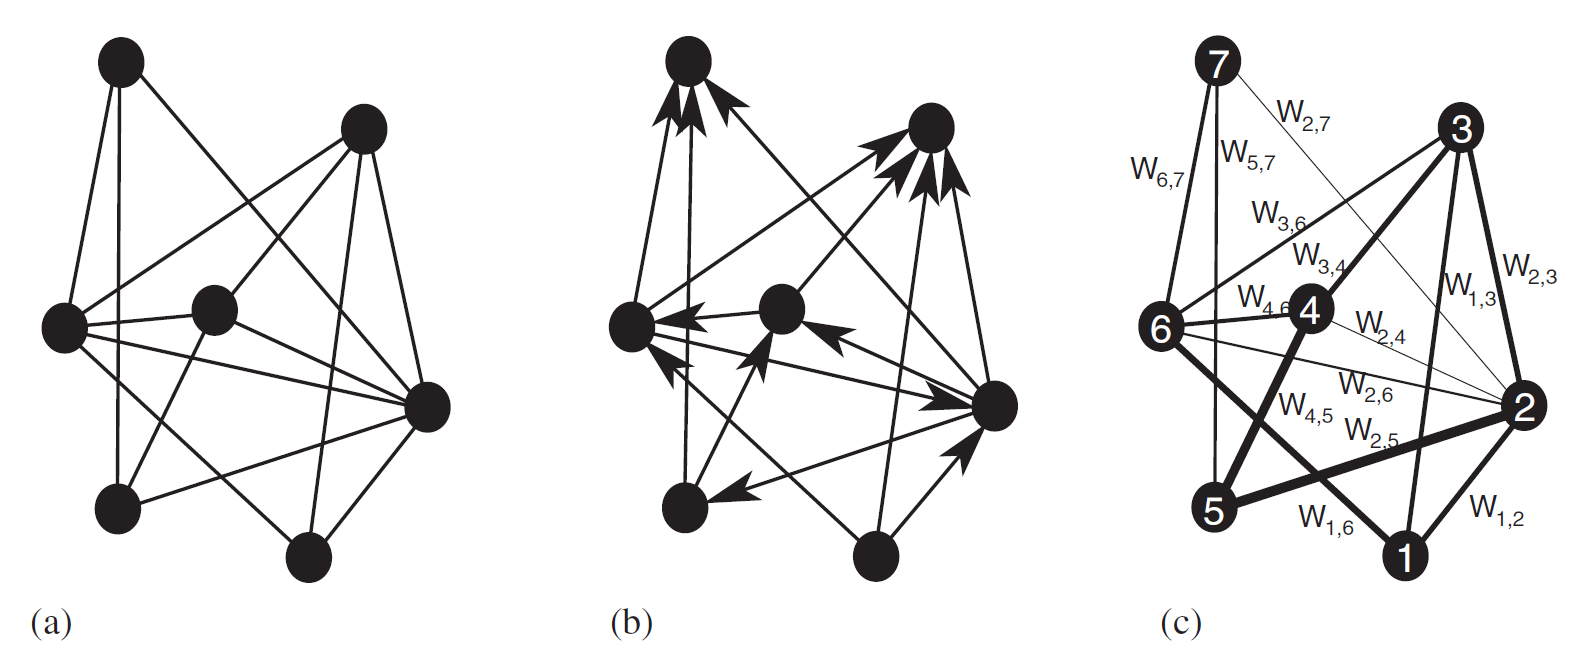
\includegraphics[scale=0.75]{fig/CH2/graph_types_03.PNG}
		\caption{A visual representation of a (a) undirected, (b) directed, and (c) weighted undirected graph, with $N = 7$ and $K = 14$ \citep{boccaletti2006complex}. Typically, the dots represent the nodes and the lines represent the links. The links with the undirected graph has no direction, in contrast with the directed graph, where a direction is indicated. Finally, the links within the undirected weighted graph have an associated weight $w^G_{ij}$. The thickness of the line (link) indicates the weight value assigned to that link. Also, the weight value indicates the degree of connectedness between the nodes.}
		\label{fig:ch2_graph_types}
	\end{center}	
\end{figure}

Now that the necessary notations and definitions are defined, the project can explain how the proposed framework can apply complex network analysis in a fraud prevention context. From here, the term \textit{network analytics} will be used as an umbrella term when referring to an analysis that contains either components of graph theory, social network analysis, or complex network analysis. 

As mentioned before, network analytics has been useful in solving network-related optimisations problems and establishing or quantifying if a relationship exists between the actors in the social network. However, knowing what can be done from network analytics, one needs to ask whether it is an applicable analysis method in a financial fraud context (for example, money laundering) and whether detection systems will benefit from the analysis. \citet{baesens2015fraud} explains the concepts of fraud from a sociological point of view. They explain that if fraud is a social phenomenon, then the concept of \textit{homophily} applies. Homophily is described as the phenomenon where people tend to associate with others whom they perceive as similar to themselves in some way \citep*{newman2018networks}. Therefore, if homophily is applicable, fraudsters will likely associate themselves with other fraudsters due to similar \textit{characteristics} or \textit{behavioural patterns}. 

As mentioned before, one of the steps of a fraud prevention/detection system is to identify emergent patterns that indicate fraudulent or suspicious behaviour (For example, step 1 of phase 2 of the general anti-money laundering process, Figure \ref{fig:ch2_aml_process}). In identifying these patterns, certain characteristic's or behavioural patterns are highlighted, which increases the probability of an event (for example, an account) as being  fraudulent. To illustrate this concept, consider the toy example of two banking clients: Client X is a 54-year-old man that works at an accounting firm and makes an average of 20 wire transfers a month with an average amount of R15 000 per wire transfer. Client Y is a 31-year-old woman that works at a gym and makes an average of 6 wire transfers a month with an average amount of R3 000 per wire transfer. Assuming the bank only had the above data on all their clients, then according to the bank anti-fraud process, it could determine that males above the age of 35 that works for a financial institution and makes more than 15 wire transfers a month of which has an average value more than R10 000 per wire transfer are deemed high risk and could be possible future fraudsters. Therefore, client X will receive a higher fraud risk score than client Y because he fits the profiling better. 

In the example above, the focus should not be the anti-fraud process but the \textit{data} provided to this process. According to the example, the feature's ($\boldsymbol{x}_i$) that the bank had to use to classify the fraud risk (probability of a client being fraudulent in the future - $y_i$) was the age, gender, average number of wire transfers per month, and average value of wire transfers per month of their clients. Currently, the bank is only considering customer information (demographics) and transactional information of the clients. If other dimensions that enrich the existing data are introduced, could this possible improve the risk classification of the existing anti-fraud process? The project proposes that \textit{network analytics} can add these additional dimensions.

If a weighted undirected client network or graph $G^W$ of is constructed at time $t$, denoted as $G^W(t) = (\mathcal{N}_t,\mathcal{L}_t,\mathcal{W}^G_t)$, certain features or metrics can be extracted from the network. In this graph, the links $\mathcal{L}$ represent the transactions connecting the different banking clients, which represent the nodes $\mathcal{N}$. How the weights are assigned to each link in the graph can be done in various ways. 

The type of weight discussed earlier is referred to as a \textit{numeric weight}. As mentioned before, a high value for this type of weight indicates a close affiliation between the nodes. \citet{baesens2015fraud} defined three other types of weights, namely, \textit{binary weight}, \textit{normalised weight}, and \textit{Jaccard weight}. A binary weight is the same as a standard network representation, i.e., the weight value is either 1 or 0  depending on if there is or is not a link present between two nodes, respectively. A normalised weight is a variant of the numeric weight where all the outgoing links weight (assuming we have a directed network) sum up to 1. Finally, the Jaccard weight is a measure of how ``social'' two connected nodes are \citep*{gupte2012measuring}. Formally, the weight $w_ij$ is calculated using the formula $\frac{|\Gamma(n_i) \cap \Gamma(n_j)|} {|\Gamma(n_i) \cup  \Gamma(n_j)|}$, where $\Gamma(n_i)$ and $\Gamma(n_i)$ is the number of events nodes $i$ and $j$ attended. For the current graph, let us assume the weights are defined numerically.       

\citet{baesens2015fraud} mentions that there are three types of analysis techniques in which the main metrics that measure the impact of the social environment on the nodes of interest in a graph are extracted. These techniques and a brief description of each are listed below. 

% Explain each of these!
\begin{enumerate}
    \item \textit{Neighbourhood metrics}: These types of metrics aim to characterise the target of interest-based its direct associates. The \textit{n-order} neighbourhood, nodes that are $n$ ``hops'' away from the node of interest, is used to generate these metrics. The first order ($n = 1$) or \textit{egonet} is commonly used as the selected neighbourhood since scalability issues arise when a $n > 1$ neighbourhood is chosen in large networks.   
    \item \textit{Centrality metrics}: These measures try to quantify an individual's importance in a social network \citep{boccaletti2006complex}. Typically, centrality metrics consider the entire network structure or subgraph when measures are extracted. 
    \item \textit{Collective inference algorithms}: This analysis technique is essential for propagating or diffusing information through the network. For example, if we have a network where only certain nodes (banking clients) are labelled to be money launderers and others legitimate.  Fraud analysis can use collective inference algorithms to infer a probability that an unlabelled node is more likely to be a  money launderer or legitimate client based on the known information of the graph. Using the previous example, as opposed to neighbourhood and centrality metrics, collective inference algorithms compute the probability that a node is exposed to money laundering activity and quantify the ``influence'' the criminal act has on the unlabeled nodes.    
\end{enumerate}

Table \ref{tab:ch2_sna_metrics}summarises the most commonly used metrics derived using the above three analysis methods. The definitions and notation of each of the table's metrics were primarily obtained by \citet{boccaletti2006complex, baesens2015fraud,} and \citet*{humpherys2017foundations}. In addition, there are other network metrics mentioned, such as link density, clustering coefficient, modularity, motifs, and efficiency. However, we will primarily focus on the metrics mentioned in Table \ref{tab:ch2_sna_metrics} for the project. 

Returning to our weighted undirected client network or graph $G^W(t)$, where the nodes represent the banking clients, and the links represent the transactions made by the clients, we have established that it will be possible to extract network metrics from this graph that could give insight into  a clients influence ability, connectives, importance, etc. The previous section established that machine learning is the main field dedicated to the broad premise of learning from data and that several learning paradigms were developed to act as a framework to encapsulate this premise. As mentioned before, supervised learning is the learning type that is the paper's main focus since it aims to predict the probability that a banking client will commit money laundering in the future using a set of defined input features. A critical question that the paper needs to consider is if including the network metrics as inputs to the supervised model will increase the model's overall performance? This question is posed due to the possibility of presenting the classification model with the adjacency matrix, in vector form $\bold{a} = \{a_{1,1}, a_{1,2}, \ldots, a_{n,n} \}$, as an input feature, along with the other useful input features. If the classifier is optimal, then it would be able to detect any class of patterns, and it would be able to describe the system as a network, then the exercises of building a network and extracting network metrics would be meaningless. \citet*{zanin2016combining} asked the same question and illustrated with a numeric experiment how this hypothesis is easily disproved. In short, for \textit{part one} of the experiment, they sampled 20 000 random networks, each having $N = 10$ and a link density of 0.3. Then two topological metrics, efficiency and clustering coefficient, were extracted from each network. For \textit{part two} of the experiment, they input the adjacency matrices of the sampled networks to an artificial neural network trained to recover the obtained metric values. For the \textit{third part} of the experiment, they linearly fitted both values (the true topological values and estimated values produced by the artificial neural network) and calculated the coefficient of determination $R^2$ for a range of different hidden neurons. In each case, the $R^2$ value obtained was minimal ($<0.04$), proving that the model could not recover the true topological metrics. \citet{zanin2016combining} mentioned that the goal of the simple numeric experiment was to illustrate that a single learning algorithm is not sufficient to deal with the structure of a complex system. Therefore, the complex network approach adds important value to the study of complex systems, which cannot be obtained by machine learning alone. \citet{zanin2016combining} concluded by saying that it is possible that complex network analysis and machine learning can be used synergistically and gives examples where researchers used machine learning and complex networks to create classification models in the biomedical and engineering fields. 

In conclusion to this chapter, the project will aim to provide evidence that supports the findings of \citet{zanin2016combining} - that combining complex network analysis and machine learning, better money laundering classifiers can be constructed. This chapter formed a critical part in the project since, firstly, adequate knowledge of the problem - money laundering needed to be established. Therefore, understanding the money laundering process and its known forms is essential for the solution generating process. Secondly, understanding the existing techniques in which money laundering is combated (anti-money laundering processes) is essential for the project purpose (that could provide insight into improving anti-money laundering processes). And finally, introducing both machine learning and complex network analysis and how they can be used synergistically to produce stronger, more robust classification models. The next chapter will discuss the methodology implemented to test the projects hypothesis.     


% Please add the following required packages to your document preamble:
% \usepackage{multirow}
\begin{sidewaystable}
\begin{adjustbox}{scale=0.65,center}
\begin{tabular}{ccll}
\hline
\textbf{Analysis technique}                                                      & \textbf{Metric}                                                                                    & \multicolumn{1}{c}{\textbf{Short description of metric}}                                                                                                                                                                                                                                                                                                                                                                                                                                                                                                                                                                                                       & \multicolumn{1}{c}{\textbf{Formula to caculate metric or metric symbol}}                                                                                                                                                                                                                                                                                                                                                                                                                                                                                               \\ \hline
\multirow{7}{*}{\begin{tabular}[c]{@{}c@{}}Neighborhood \\ metrics\end{tabular}} & \multicolumn{1}{c|}{Degree}                                                                        & \multicolumn{1}{l|}{\begin{tabular}[c]{@{}l@{}}The degree $k_i$ of node $i$ is the number\\ of links incident with the node.\end{tabular}}                                                                                                                                                                                                                                                                                                                                                                                                                                                                                                                     & $k_i = \sum_{j \in \mathcal{N}}^{}a_{ij}$                                                                                                                                                                                                                                                                                                                                                                                                                                                                                                                              \\ \cline{2-4} 
                                                                                 & \multicolumn{1}{c|}{Traingle}                                                                      & \multicolumn{1}{l|}{\begin{tabular}[c]{@{}l@{}}The number of cycles ($C_k$) that has $k = 3$\\  of  which node $i$ forms part of.\end{tabular}}                                                                                                                                                                                                                                                                                                                                                                                                                                                                                                                & $triangle(n_i)$                                                                                                                                                                                                                                                                                                                                                                                                                                                                                                                                                        \\ \cline{2-4} 
                                                                                 & \multicolumn{1}{c|}{Density}                                                                       & \multicolumn{1}{l|}{\begin{tabular}[c]{@{}l@{}}The density of a graph is the ratio of the number of edges \\ and a number of possible edges. This measure\\ indicates how ``connected'' nodes in a network are to \\ each other.\end{tabular}}                                                                                                                                                                                                                                                                                                                                                                                                                 & $p(G) = \frac{2K}{N(N-1)}$                                                                                                                                                                                                                                                                                                                                                                                                                                                                                                                                             \\ \cline{2-4} 
                                                                                 & \multicolumn{1}{c|}{Strength}                                                                      & \multicolumn{1}{l|}{\begin{tabular}[c]{@{}l@{}}The sum of the weights of each edge adjacent \\ to a vertex. Also known as the degree strength.\end{tabular}}                                                                                                                                                                                                                                                                                                                                                                                                                                                                                                   & \begin{tabular}[c]{@{}l@{}}$s_i = \sum_{j=1}^{N}a_{ij}w^G_{ij}$\\ Where $s_i$ is the degree strength of node $i$.\end{tabular}                                                                                                                                                                                                                                                                                                                                                                                                                                         \\ \cline{2-4} 
                                                                                 & \multicolumn{1}{c|}{\begin{tabular}[c]{@{}c@{}}Transitivity \\ (local)\end{tabular}}               & \multicolumn{1}{l|}{\begin{tabular}[c]{@{}l@{}}Measures the probability that \\ adjacent vertices of a vertex are connected.\\ The measure is also known as the \\ \textit{clustering coefficient}.\end{tabular}}                                                                                                                                                                                                                                                                                                                                                                                                                                              & \begin{tabular}[c]{@{}l@{}}$C^W_i = \frac{1}{s_i(k_i-1)}\sum_{j,h}\frac{w^G_{ij}+w^G_{ih}}{2}a_{ij}a_{ih}a_{jh}$\\ Where $C^W_i$ provides the locally weighted transitivity of node $i$.\end{tabular}                                                                                                                                                                                                                                                                                                                                                                  \\ \cline{2-4} 
                                                                                 & \multicolumn{1}{c|}{\begin{tabular}[c]{@{}c@{}}Relational \\ neighbour\end{tabular}}               & \multicolumn{1}{l|}{\begin{tabular}[c]{@{}l@{}}The relative number of neighbours that is allocated\\ to a specific class, for example, a neighbourhood node can \\ have the label HC that indicates that they are an honest \\ client or they can have the label MLC, which indicate that\\ the client is a money-laundering client.\end{tabular}}                                                                                                                                                                                                                                                                                                             & \begin{tabular}[c]{@{}l@{}}$P(class|n_i) = \frac{1}{Z}\sum_{n_j \in {Neighbourhood_n}_i} w^G_{ij}$\\ Where $Z$ is a normalisation factor, ${Neighbourhood_n}_i$ is the\\ $1^{st}$ degree neighbourhood of node $i$, and $class$ is the label \\ of interest.\end{tabular}                                                                                                                                                                                                                                                                                              \\ \cline{2-4} 
                                                                                 & \multicolumn{1}{c|}{\begin{tabular}[c]{@{}c@{}}Probabilistic \\ relational neighbour\end{tabular}} & \multicolumn{1}{l|}{\begin{tabular}[c]{@{}l@{}}This metric is an extension of the relational neighbour\\ metric, whereas the weight, $w^G_{ij}$ is defined\\ as the probability of node $j$ (a neighbour of node $i$)\\ belonging to a certain class. For example,  the probability \\ of node $n_i$ being a money-laundering client is equal\\ to the sum of the probabilities of neighbouring nodes, \\ which are classified as money launderers.\end{tabular}}                                                                                                                                                                                              & \begin{tabular}[c]{@{}l@{}}$P(class|n_i) = \frac{1}{Z}\sum_{n_j \in {Neighbourhood_n}_i} w^G_{ij}$\\ Where $w^G_{ij} = P(class|n_j)$.\end{tabular}                                                                                                                                                                                                                                                                                                                                                                                                                      \\ \cline{2-4} 
\multirow{5}{*}{\begin{tabular}[c]{@{}c@{}}Centrality \\ metrics\end{tabular}}   & \multicolumn{1}{c|}{Geodesic path}                                                                 & \multicolumn{1}{l|}{The walk that has the smallest length between nodes.}                                                                                                                                                                                                                                                                                                                                                                                                                                                                                                                                                                                      & $min(d(n_i,n_j))$                                                                                                                                                                                                                                                                                                                                                                                                                                                                                                                                                      \\ \cline{2-4} 
                                                                                 & \multicolumn{1}{c|}{\begin{tabular}[c]{@{}c@{}}Closeness \\ centrality\end{tabular}}               & \multicolumn{1}{l|}{\begin{tabular}[c]{@{}l@{}}The average distance from node $i$ to all other nodes\\ in the graph. Closeness centrality is the reciprocal\\ of \textit{farness}.\end{tabular}}                                                                                                                                                                                                                                                                                                                                                                                                                                                               & \begin{tabular}[c]{@{}l@{}}$c(n_i) = \left [\frac{\sum_{j=1;j\neq i}^{N}d(n_i,n_j)}{N-1}\right ]^{-1}$\\ Very large values of $d(n_i,n_j)$ are often excluded due to $\lim_{x \to -\infty}\left (\frac{1}{x} \right )$.\end{tabular}                                                                                                                                                                                                                                                                                                                                    \\ \cline{2-4} 
                                                                                 & \multicolumn{1}{c|}{\begin{tabular}[c]{@{}c@{}}Eigenvector \\ centrality\end{tabular}}             & \multicolumn{1}{l|}{\begin{tabular}[c]{@{}l@{}}The eigenvector centrality score corresponds to the  \\ values of the first eigenvector of the graph adjacency matrix. \\ Therefore, it measures the importance of nodes in a \\ network using the adjacency and eigenvector matrices.\end{tabular}}                                                                                                                                                                                                                                                                                                                                                            & \begin{tabular}[c]{@{}l@{}}$\Upsilon \vec{C_{\mathrm{IV}}}=\boldsymbol{A}\vec{C_{\mathrm{IV}}}$\\ Where $\vec{C_{\mathrm{IV}}}$ is the eigenvector, and $\Upsilon$ the eigenvalue.\end{tabular}                                                                                                                                                                                                                                                                                                                                                                        \\ \cline{2-4} 
                                                                                 & \multicolumn{1}{c|}{Betweenness}                                                                   & \multicolumn{1}{l|}{\begin{tabular}[c]{@{}l@{}}The betweenness metric counts the number times a\\ node lies on the geodesic between any two nodes\\ in the network graph.\end{tabular}}                                                                                                                                                                                                                                                                                                                                                                                                                                                                        & \begin{tabular}[c]{@{}l@{}}$b(n_i) = \sum_{j\neq h \neq i}^{}\frac{g_{jh}(n_i)}{g_{jh}}$\\ Where $g_{jh}$ is the total number of shortest paths from \\ node $j$ to node $h$ and  $g_{jh}(n_i)$ is the number of \\ those paths that pass through node $i$.\end{tabular}                                                                                                                                                                                                                                                                                               \\ \cline{2-4} 
                                                                                 & \multicolumn{1}{c|}{Graph theoretic center}                                                        & \multicolumn{1}{l|}{\begin{tabular}[c]{@{}l@{}}The node with the smallest maximum distance to\\ all other nodes in the network.\end{tabular}}                                                                                                                                                                                                                                                                                                                                                                                                                                                                                                                  & \begin{tabular}[c]{@{}l@{}}$G_{centre} = min(max(path(n_i,n_j)))$\\ Where $path(n_i,n_j)$ gives the length of the path(s)\\ from node $i$ to $j$ and $\{i,j = \{1,2, \ldots, N \}, i \neq j\}$.\end{tabular}                                                                                                                                                                                                                                                                                                                                                           \\ \cline{2-4} 
\begin{tabular}[c]{@{}c@{}}Collective inference \\ algorithms\end{tabular}       & \multicolumn{1}{c|}{PageRank}                                                                      & \multicolumn{1}{l|}{\begin{tabular}[c]{@{}l@{}}The PageRank algorithm is an algorithm that ranks the\\ nodes in a graph by some importance. The PageRankalgorithm forms \\ the basis of Google's search engine algorithm for ranking web pages. \\ Using web pages as an example, the algorithm determines the probability \\ of a web surfer visiting a  specific web page. The probability of visiting a \\ web page is called its pagerank. Referring to the above example, PageRank \\ can establish the propagation of page influence through the network. \\ Similarly, the algorithm can be used to propagate fraud throughout a network.\end{tabular}} & \begin{tabular}[c]{@{}l@{}}$\bold{p}(0) = \frac{1}{N}\bold{1}$;\\ $\bold{p}(t+1) = \alpha(D^{-1}\bold{A})^T\bold{p}(t) + \frac{1-d}{N}\bold{1}$\\ Where $\bold{p}(t) = \{p_1(t), \{p_2(t), \ldots, \{p_N(t)\}^T$, \\ $\bold{1}$ is a vector of $N$ ones, $D$ is a diagonal matrix, \\ and $\alpha$ is the damping factor\footnote{The expression is in matrix form. Also, the expression is the modified version of the original PageRank expression. This version accounts for pages with no outbound links and incorporates the boredom factor.}.\end{tabular} \\ \cline{2-4} 
\end{tabular}
\end{adjustbox}
\caption{Summary of the main metrics produced by the three types of analysis techniques used to analyse the social environment of nodes in a graph:  i) neighbourhood metrics, ii) centrality metrics, and iii) inference algorithms. The metrics produced by each analysis technique is given along with a short description of the metric and an expression used to calculate the metric.}
\label{tab:ch2_sna_metrics}
\end{sidewaystable}











%%%%%%%%%%%%%%%%%%%%%%%%%%%%%%%%%%%%%%%%%%%%%%%%
%
% start writing
%
%%%%%%%%%%%%%%%%%%%%%%%%%%%%%%%%%%%%%%%%%%%%%%%%

\chapter{Methodology} \label{ch3_heading}

%[Introduction to contents of chapter - Data, Feature Engineering, and Modelling]
The previous chapter gave a detailed introduced money laundering, machine learning and network analytics. The chapter concluded that machine learning and network analytics could synergistically improve anti-money laundering detection processes. The methodology followed to test the project's hypothesis and answer the research question posed in chapter \ref{ch1_heading} is disclosed in the following chapter. Therefore, a detailed explanation of Figure\ref{fig:ch1_project_framework}, the high-level project overview, is provided in the chapter. The chapter is divided into three sections. The first section aims to provide all the relevant information about the data simulator (AMLSim) and how the project used it to generate the raw data for the project. The second section provides the details of the feature engineering process and its outcome - three structured data sets (network features data set, transactions feature data set, and combined features data set). The final section explains the modelling process. The section describes the models used, the pre-processing of the data, the hyper-parameter tuning process, and the model evaluation process.

\section{Data} \label{ch3_sub_heading_data}

%[What data was used? How was it obtained?]
For the projects application of network analytic's and machine learning, adequate data is needed. To obtain client transactional data from financial institutions (such as banks) is very challenging due to legal and competitive reasons \citep*{watkins2003tracking}. Therefore, obtaining actual client transactional data for research is complicated. A substitute for real-world client transactional data is synthetic data generated using a simulator. \citet*{banks1998handbook} defined simulation as being the imitation of the operations of a real-world process or system over time. Therefore, using simulation as a means to generate synthetic data that represents real-world behaviour is a sophisticated solution to obtaining the data needed for the project's purpose \citep*{lopez2016applying}. Also, simulation provides the advantages of creating different situations or scenarios, allowing the analyst to test and evaluate models under different conditions. However, the data simulator should be complex enough to mimic real-world behaviour experienced by anti-money laundering processes to conduct adequate research. For this reason, the project used a simulator developed by MIT \& IBM, called AMLSim\footnote{The GitHub page for AMLSim is found at: \url{https://github.com/IBM/AMLSim}}. AMLSim is an intricate data simulator with certain functionalities that did not apply to the project. Therefore, the project only focused on the simulator's functionalities that were useful for the project research goal. The following section explains, in detail, step one in the project's high-level overview (Figure \ref{fig:ch1_project_framework}).

%[What is AMLSim?]
AMLSim is a multi-agent simulation platform specifically created to generate synthetic data for anti-money laundering research purposes \citep*{AMLSim}. In the simulator, the agents represent bank accounts and the agent's behaviour is defined to transfer money to other agents (bank accounts). A small number of agents are tasked to participate in illegal money laundering activities. More specifically, how the ``criminal'' agents perform the money laundering is based on real-world money laundering typologies or patterns. On a high level, the functioning of the simulator is divided into two stages. The first stage generates a network of bank accounts linked by transactions. The second stage uses a secondary simulator called PaySim to produce a time series of transactions. Using Figure \ref{fig:ch3_amlsim}, these two phases of AMLSim are explained in further detail.

\begin{figure}
	\begin{center}
		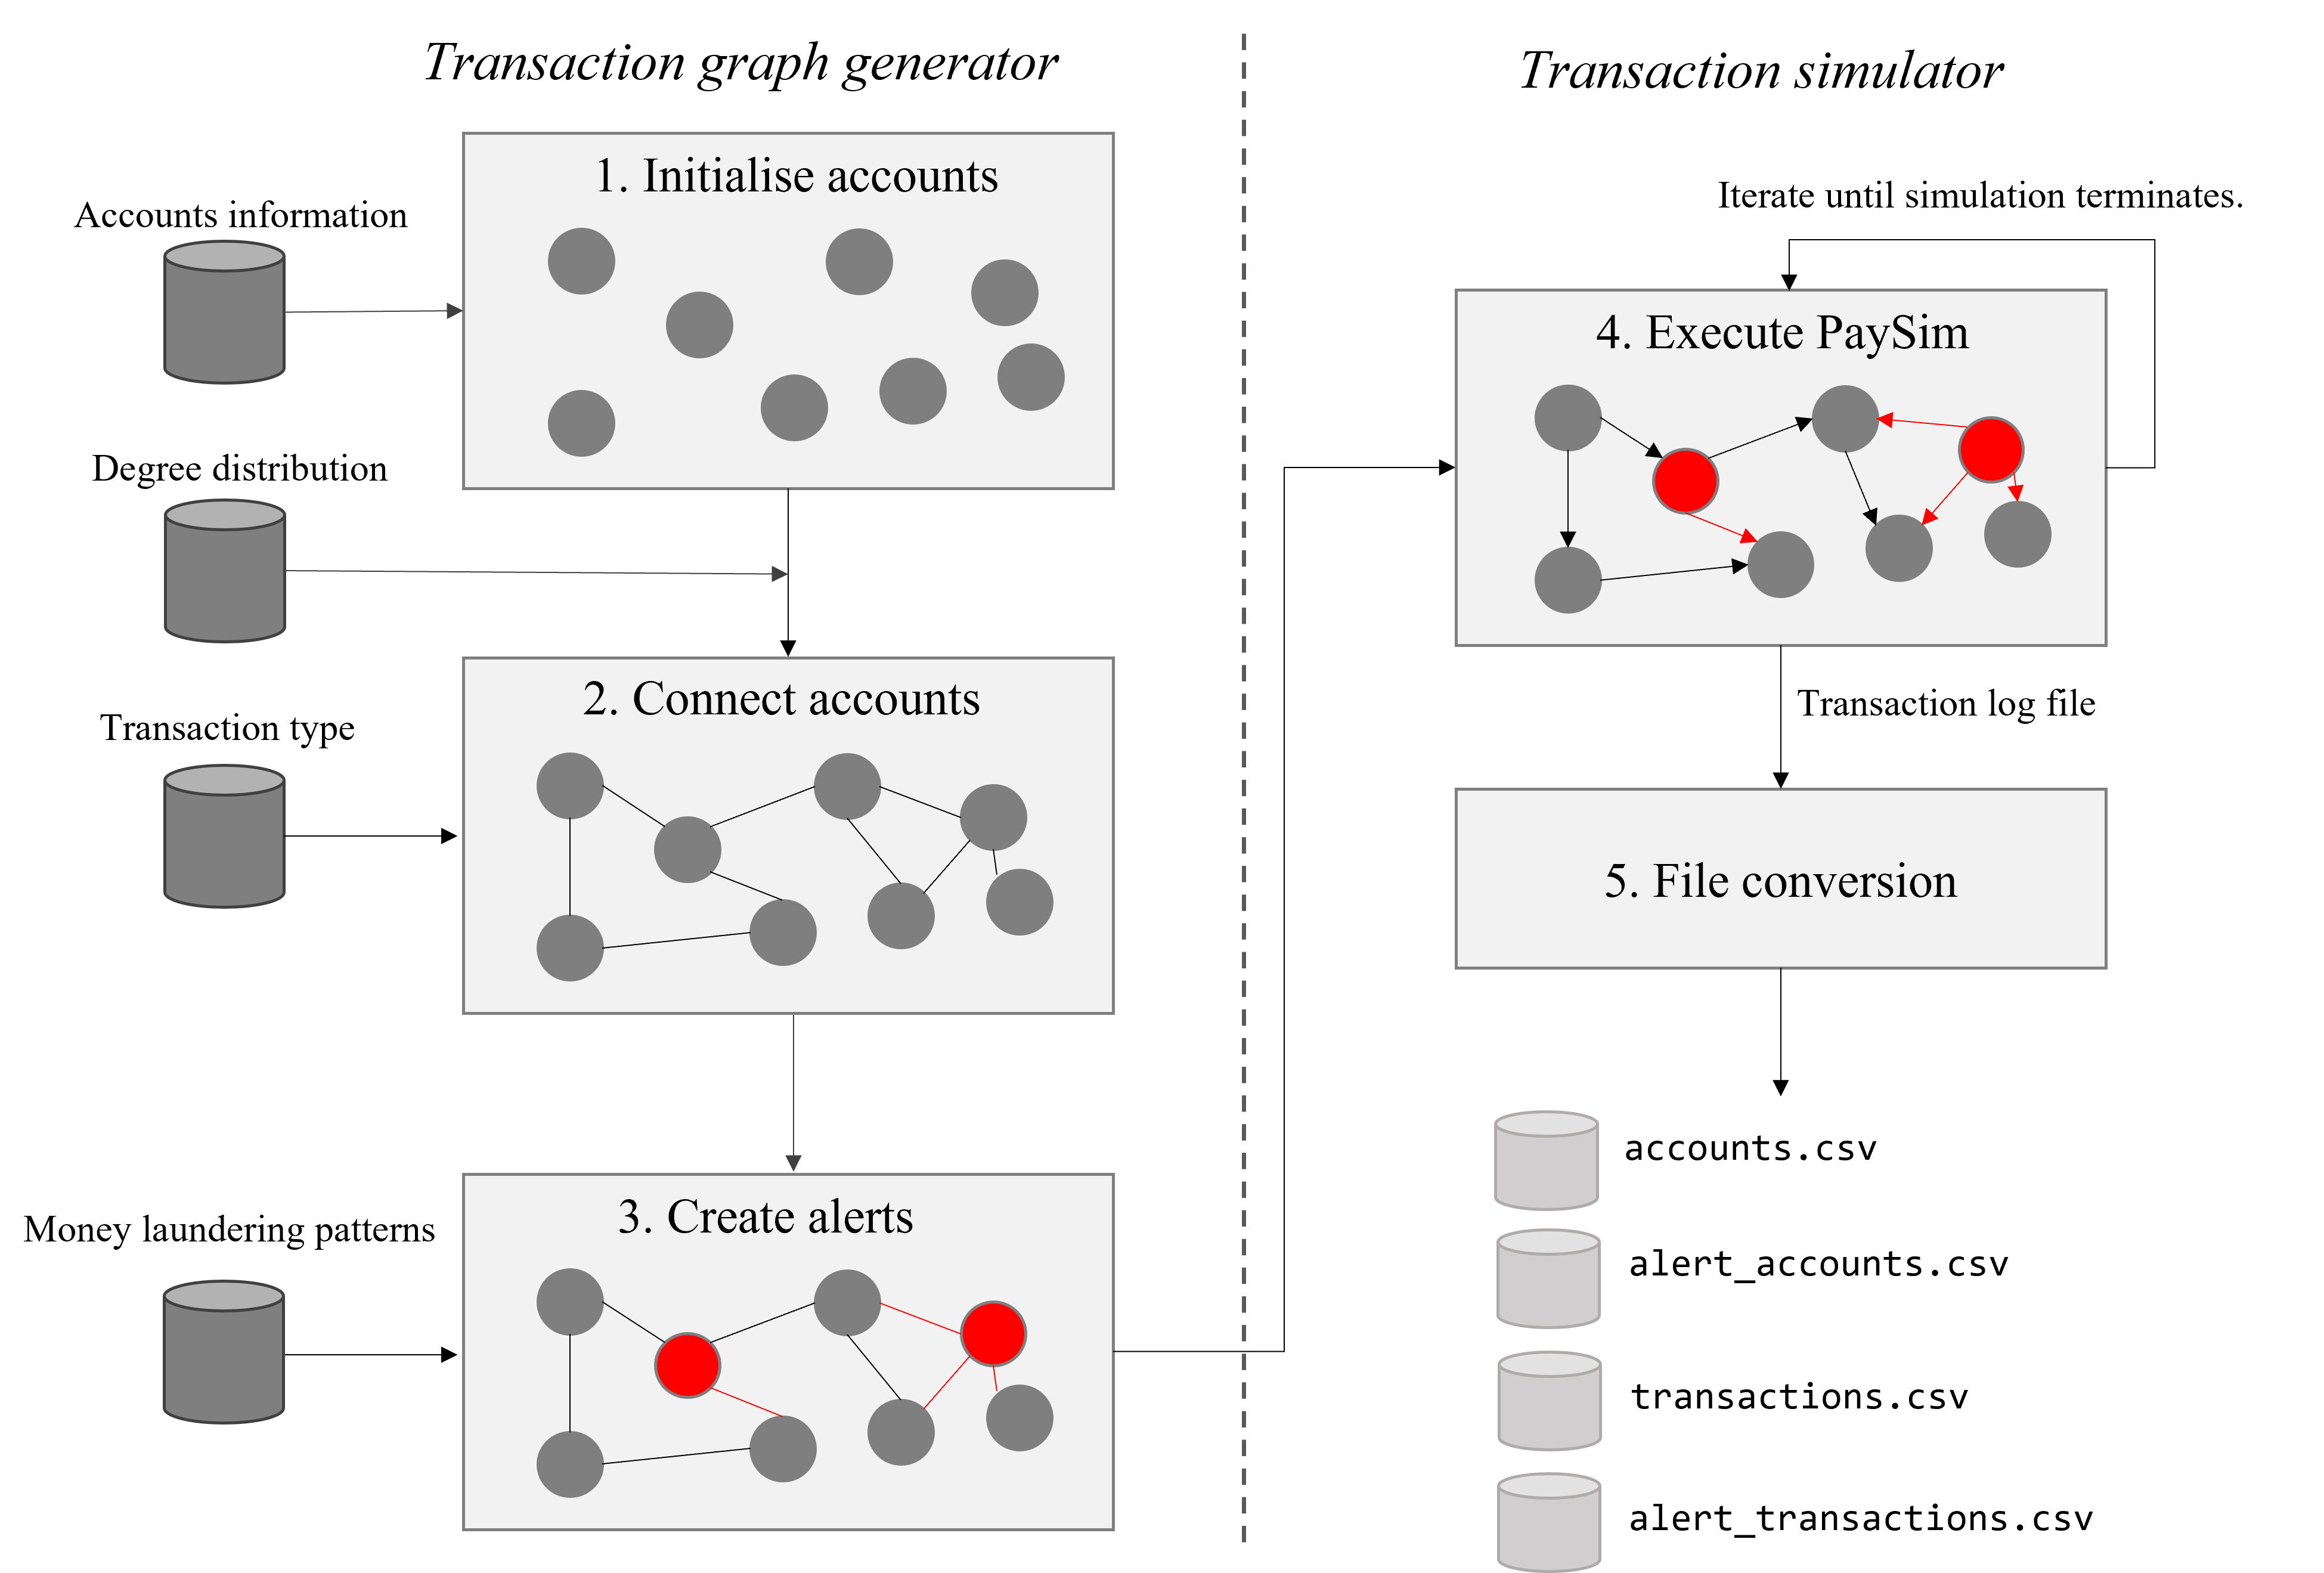
\includegraphics[scale=0.55]{fig/CH3/AML_SIm.PNG}
		\caption{A visual representation of the two stages and sub-stages in the functioning of AMLSim \citep{AMLSim, weber2018scalable, lopez2016applying}}
		\label{fig:ch3_amlsim}
	\end{center}	
\end{figure}

% [How does AMLSim work?]
% [How does AMLSim work? - inputs]
The first phase is referred to as the \textit{transaction graph generator} phase. The inputs files need to be explained before explaining this phase in more detail. The input files, along with a short description of each, are as follows:

\begin{enumerate}
    \item \textit{Transaction type}: The file specifies the type of transactions in the simulation. The types of transactions defined in the simulator are credit, deposit, wire transfer, and check. Also, the probability of each transaction type occurring is specified in the file.
    
    \item \textit{Account information}: Provides information on the bank accounts. For example, the number of accounts the simulator should generate, the initial balance for the accounts, and the behaviour the accounts should follow (discussed in further depth later on).
    
    \item \textit{Degree distribution}: Specifies the out-degree and in-degree of the bank accounts, which corresponds to the number of payments made and received by bank accounts respectfully. 
    
    \item \textit{Money laundering patterns}: The file provides the details of the money laundering activities that need to occur in the simulation. For example, the frequency of each money laundering typology (discussed in further depth later on), the time it takes to complete a money laundering activity, the money laundering amount, and the number of accounts involved in the money laundering activity.    
    
\end{enumerate}

% [How does AMLSim work? - stage 1]
The transaction graph generator consists of three sub-phases. The first sub-phase initialises a network with the properties specified in the accounts information file. In the network, the accounts are represented by vertices. After the network's vertices are generated, the second sub-phase generates the connections (edges) between the vertices according to the degree distribution and transaction type input files. The final sub-phase of the transactional graph generator is to incorporate fraudulent transactions into the network according to the metrics specified in the money laundering patterns input file. The output of the transaction graph generator is an attributed network that contains the account properties and transactional behaviour of all banking accounts (honest and money-laundering). To clarify, the transactional graph generator does not assign any values to transactions made between clients. It only specifies the characteristics or properties of the nodes (banking accounts) and edges (transactions) according to the respective input files. The values for each transaction is generated in the second phase of AMLSim - the \textit{transaction simulator}. More specifically, a time series of transactions are created using PaySim. Before discussing how the two phases merge into one another, a short introduction to PaySim is required.

% [How does AMLSim work? - stage 2 - PaySim]
PaySim is a financial simulator designed initially to simulate mobile money transactions \citep{lopez2016applying}. In short, mobile money transactions is when funds are sent or received using a mobile phone and is a type of electronic fund transfer (EFT) \citep*{money2021transfer}. The PaySim transactional simulator was built using samples of actual transactional data. As mentioned before, PaySim accomplishes the replication of real-world transactional behaviour by using agent-based simulation. An agent (represented by a bank account) is placed in an environment that requires it to make particular decisions depending on the information it receives. The agent's choice to execute a transaction is based on statistical distributions. Also, each agent has an assigned probability value, which indicates the agents' probability of performing transactions in future steps. Altogether, the \textit{input information} the agent receives, the \textit{statistical distributions} (to execute a transaction or not), and the \textit{probability value} of making future transactions were defined when PaySim was initially built. These pre-defined simulation parameters best represent the behaviour of real-world transaction transfers when presented to the agent-based modelling environment. 

% [How does AMLSim work? - stage 2 and outputs]
Now that an initial understanding of PaySim is established, the discussion can continue how it functions within AMLSim. The transaction simulator consists of three stages. These stages are essentially the stages of executing the PaySim simulator. The first stage, the \textit{initiation stage}, takes as input the attributed network, generated by the transaction graph generator, and extracts all the information required for the agent-based simulation. The second stage is the \textit{execution stage}. This stage is where the actual simulation takes place. Based on the input parameters (extracted from the attributed network), the agents will have sufficient knowledge of their role in the simulation. For example, the number of transaction's they can make in the simulation time, their initial balance, and their distributional properties (which entails the probabilities of executing a certain action). The third sub-stage is the \textit{finalisation stage}. After each agent has completed their assigned roles, the simulation is terminated, and the results are saved. Several output files are generated upon the termination of PaySim. The only output file used by AMLSim is the transaction log file. In short, the transaction log file provides a record of each transaction made and the meta-data for the transaction. Finally, the log file is converted to a more user-friendly format along with additional accounts information. The final output of the AMLSim simulation are four \texttt{csv} files: \texttt{accounts.csv}, \texttt{alert\_accounts.csv}, \texttt{transactions.csv}, and \texttt{alert\_transactions.csv}. These files would serve as the raw data for the project. The exploratory data analysis (EDA) provides a more detailed explanation of these raw data files, discussed later in the section. 

%[What input parameters were used, in AMLSim, to generate the data for the project?]
Since an understanding of AMLSim is established, more focus can be placed on the contents of the input files (transaction type, account information, degree distribution, and money laundering patterns) specified for the project's purposes. Establishing which input parameters to use for the project research question was a significant challenge due to the infinite possible combinations of input parameters. There is also no clear consensus found in literature on what input parameters should be used to generate baseline anti-money laundering data \citep{pareja2020evolvegcn, AMLSim, weber2018scalable}. Luckily, \citet{AMLSim} defined several fixed input parameter folders that generate anti-money laundering data specifically compiled for testing machine learning models. Within the fixed input parameter folders are the respective simulator input files. The fixed input folders used for the training data set and the testing data set was the ``\texttt{10K}'' and ``\texttt{1K}'' folders, respectively. The only difference between the two input folders is the number of accounts used in the simulation. The ``\texttt{10K}'' folders generates approximately 10 000 accounts and the ``\texttt{1K}'' folder generates approximately 1000 accounts. The project will provide more details on the training and testing data set in section \ref{ch3_sub_heading_modelling}. Furthermore, except for the money laundering patterns input file, all the default settings for each input file were used. To understand the alteration made to this input file, an explanation of the normal and money laundering typologies defined within AMLSim needs to be established first.
% [money laundering and normal typology's - inputs to the project]

AMLSim has various normal and money laundering typologies defined. The normal typologies are \textit{periodical}, \textit{forward}, \textit{single}, \textit{fan-in}, \textit{fan-out}, and \textit{mutual}. Firstly, the \textit{periodical} typology is when account X sends funds to account Y on some periodical basis (weekly, monthly, etc.). The \textit{forward} typology is when account X transfers funds to account Y, and then account Y forwards the funds to account Z. A \textit{single} typology is when account X makes a transfer to account Y. The \textit{fan-in} and \textit{fan-out} typologies refer to when an account receives funds from multiple other accounts or when an account makes transfers to multiple other accounts, respectively. The final normal typology, \textit{mutual}, refers to when account X makes a transfer to account Y and then, shortly after some time, receives the funds back from account Y. The money laundering typologies incorporated in AMLSim are more complicated than the normal typologies. The money laundering typologies are \textit{cycle}, \textit{fan-in}, \textit{fan-out}, \textit{gather-scatter}, \textit{scatter-gather}. The \textit{cycle} typology occurs when an account transfers funds to another account, and after several other transfers involving other accounts, the funds return to the origin account. For example, account X transfers funds to account Y, and account Y transfers the funds to account Z and account Z transfers the funds back to account X (completing the ``cycle''). The \textit{fan-out} and \textit{fan-in} money laundering typologies are equivalent to that explained in the normal typologies; however, the \textit{gather-scatter} typology combines the fan-in and fan-out typologies after each other (vice versa for the \textit{scatter-gather} typology).      

% [changed values to money laundering patterns file - inputs to the project]
Now that an understanding of the normal and money laundering typologies has been established, the alteration of the default values of the money laundering patterns input file can be explained. Initially, the input file only had three money laundering typologies specified (fan-in, fan-out, and cycle). It was decided to include \textit{all} other money laundering typologies since the project research goal was to investigate how network or graph derived features impacts a classifier's performance in detecting money laundering activity among banking accounts, in \textit{general}, and not focusing on a specific set of money laundering typologies. Therefore, the added money laundering typologies were: gather-scatter and scatter-gather.

% [How did the raw data look? - EDA raw data]
After correctly configuring all input files, the AMLSim simulator was executed \textit{twice}. Firstly, to generate the training raw data (using the ``\texttt{10K}'' input folder) and a secondly to generate the testing data (using the ``\texttt{1K}'' input folder). The only difference between the two input folders is the number of accounts initialised in the simulation. Furthermore, the features generated in the output files are identical. As mentioned before, AMLSim produces the following \texttt{csv} files: \texttt{accounts.csv}, \texttt{alert\_accounts.csv}, \texttt{transactions.csv}, and \texttt{alert\_transactions.csv}. The  project did not directly use the \texttt{alert\_accounts.csv} and \texttt{alert\_transactions.csv} files in the feature engineering phase (discussed in section \ref{ch3_sub_heading_feature_engineering} ); however, they were included in the EDA conducted of the outputted raw data files. An exploratory data analysis is an essential part of any data analysis \citep*{wickham2016r}. There is no formal process or strict rules when conducting exploratory analysis. In short, the goal of an EDA is to develop an understanding of the data \citep{wickham2016r}. A high-level explanation of the process of the EDA conducted of the raw data files was: i) examining the quality of the data generated by the simulator, ii) to observe if the input parameters specified was reflected in the data, and iii) to generate questions about the data that could produce helpful insights. At first glance, there were multiple features in each raw data table that contained only singular values (repetitions of the same values). These features were removed since they would not be beneficial to analysis. There were also other reasons why some variables were excluded from the analysis. Table \ref{tab:ch3_raw_features_removed} in appendix \ref{app_1} summarises all the raw data features excluded from the analysis and why. After the data cleaning exercise, the investigation of the data continued. For each raw data table (training data set and testing data set), the project investigated the following: i) basic table characteristics (for example, the number of rows/columns, data type of each variable, etc.), ii) missing data profile (how many instances of each feature was missing), iii) Uni-variate statistics (histograms - continuous variables, frequency bar charts - discrete variables ), and iv) Bi-variate distributions (box and whisker diagrams). All statistics and visualisations generated for the EDA were done for the generated training and testing raw data files. 

% [Training set - EDA raw data]
 There were 12 043 accounts and 655 433 transactions from the raw training data set. From these accounts, 782 participated in money laundering activity ($\approx 6.5\%$ of all accounts), and 626 transactions were classified as fraudulent ($\approx 1\%$ of all transactions). Figure \ref{fig:ch3_raw_eda_train_alrt_trans_sum} shows four plots generated from the \texttt{alert\_transactions.csv} file. The bottom-left plot shows that the cycle money laundering typology is the most frequent among illicit transactions, and the gather-scatter is the least. Figure \ref{fig:ch3_raw_eda_train_alrt_trans_tx_distr} shows the distributional properties of the transaction amount (\texttt{base\_amt}) for each money laundering typology. Generally, the transactions are widely distributed among all money laundering typologies, except for the scatter-gather typology, which has much more concentrated amounts between approximately \$170 and \$190. The bottom-left plot in Figure  \ref{fig:ch3_raw_eda_train_acct_sum} shows a box and whiskers plot of the opening account balance (\texttt{initial\_deposit}) for fraudulent and non-fraudulent accounts. The two distributions seem identical for both fraud and non-fraud clients.
 
% [Testing set - EDA raw data]
There were 1446 accounts and 108 684 transactions in the raw testing data set. From these accounts, 72 participated in money laundering activity  ($\approx 5\%$ of all accounts), and 52 transactions were classified as fraudulent ($\approx 0.5\%$ of all transactions). The EDA also generated the same type of figures displayed for the training data (Figures \ref{fig:ch3_raw_eda_test_alrt_trans_sum}, \ref{fig:ch3_raw_eda_test_alrt_trans_tx_distr}, and \ref{fig:ch3_raw_eda_test_acct_sum}) for the test data. These figures are displayed in appendix \ref{app_2}. Overall, very similar characteristics are observed in the raw test data set. For example, the money laundering typology least frequent among illicit transactions is the gather-scatter typology (Figure \ref{fig:ch3_raw_eda_test_alrt_trans_sum}). Also, the transaction amount distributions for the money laundering typologies are widely spread, except for the scatter-gather typology (Figure \ref{fig:ch3_raw_eda_test_alrt_trans_tx_distr}). Finally, a slight difference between the initial balance means of fraudulent accounts and non-fraudulent accounts is observed (Figure \ref{fig:ch3_raw_eda_test_acct_sum}).


\begin{figure}
	\begin{center}
		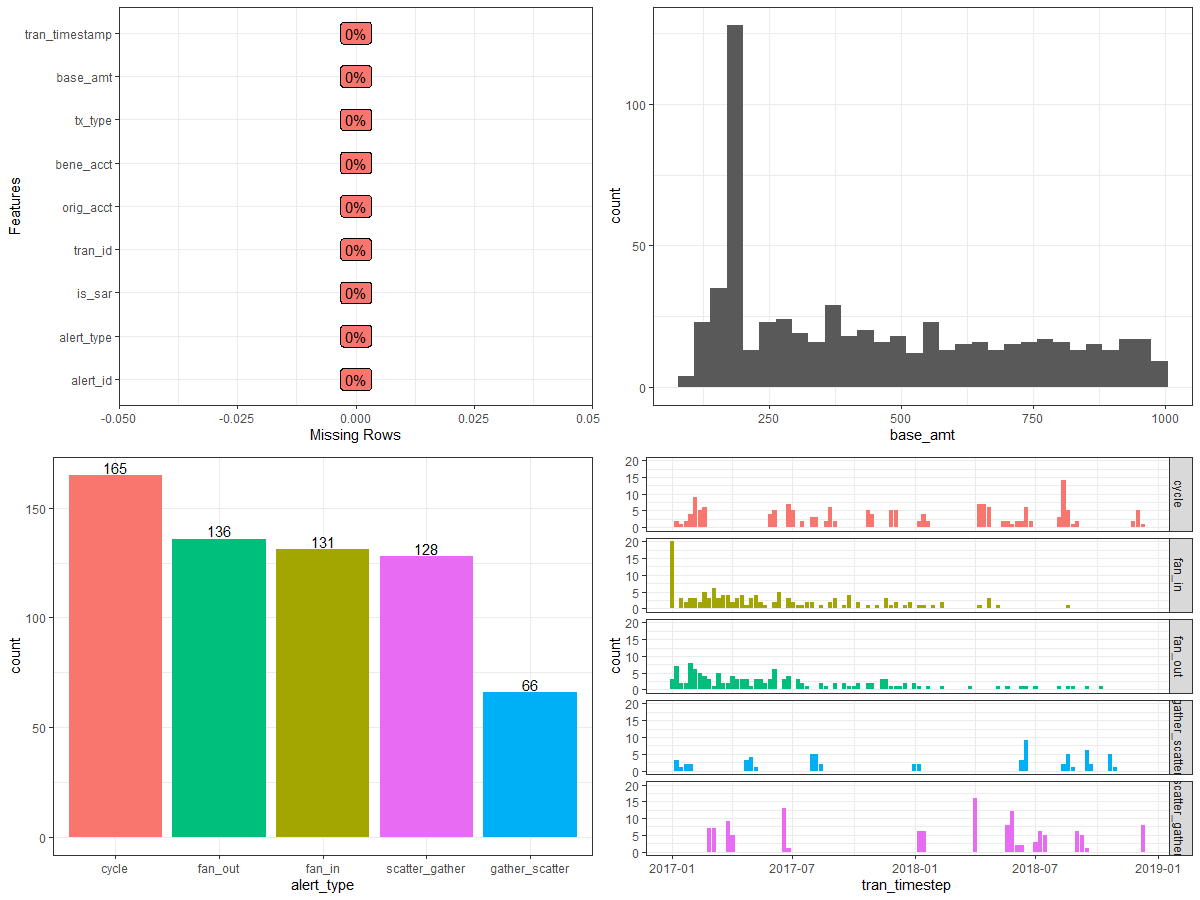
\includegraphics[scale=0.5]{fig/CH3/train_alrt_trans_summary.png}
		\caption{Example of the visualisations generated during the EDA of the training \texttt{alert\_transactions.csv} file. (top-left) The missing values profile. (top-right) Histogram of the transaction amount (\texttt{base\_amount}). (bottom-left) Frequency bar chart of the occurrences of different money laundering typologies (\texttt{alert\_type}) among the account transactions. (bottom-right) A timeline plot of when the different money laundering typologies occurred.}
		\label{fig:ch3_raw_eda_train_alrt_trans_sum}
	\end{center}	
\end{figure}

\begin{figure}
	\begin{center}
		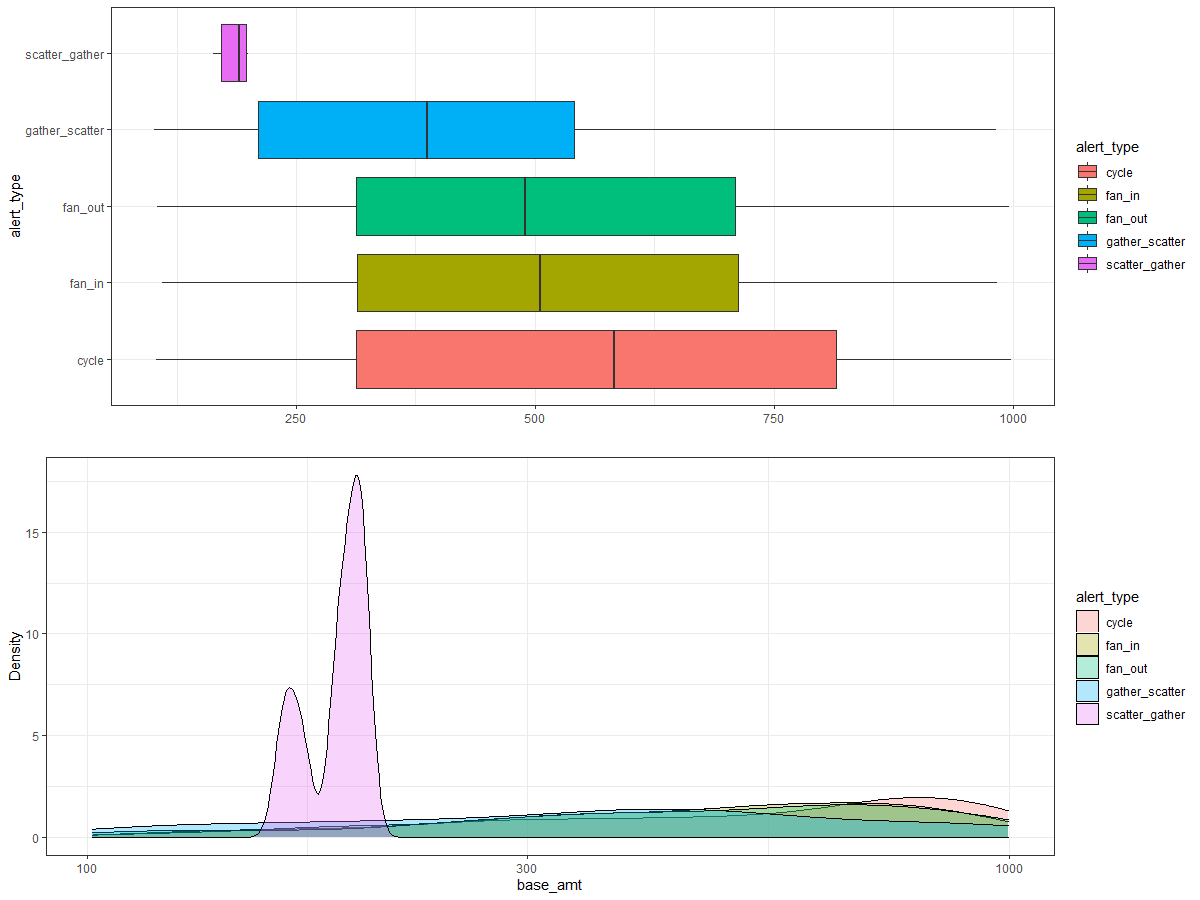
\includegraphics[scale=0.5]{fig/CH3/train_alrt_trans_tx_amount_alert_type_distribution.png}
		\caption{Both plots show the transaction amount distribution (top - box and whiskers and bottom - density plot) of transactions that were classified as being money laundering transactions for the training \texttt{alert\_transactions.csv} file.}
		\label{fig:ch3_raw_eda_train_alrt_trans_tx_distr}
	\end{center}	
\end{figure}

\begin{figure}
	\begin{center}
		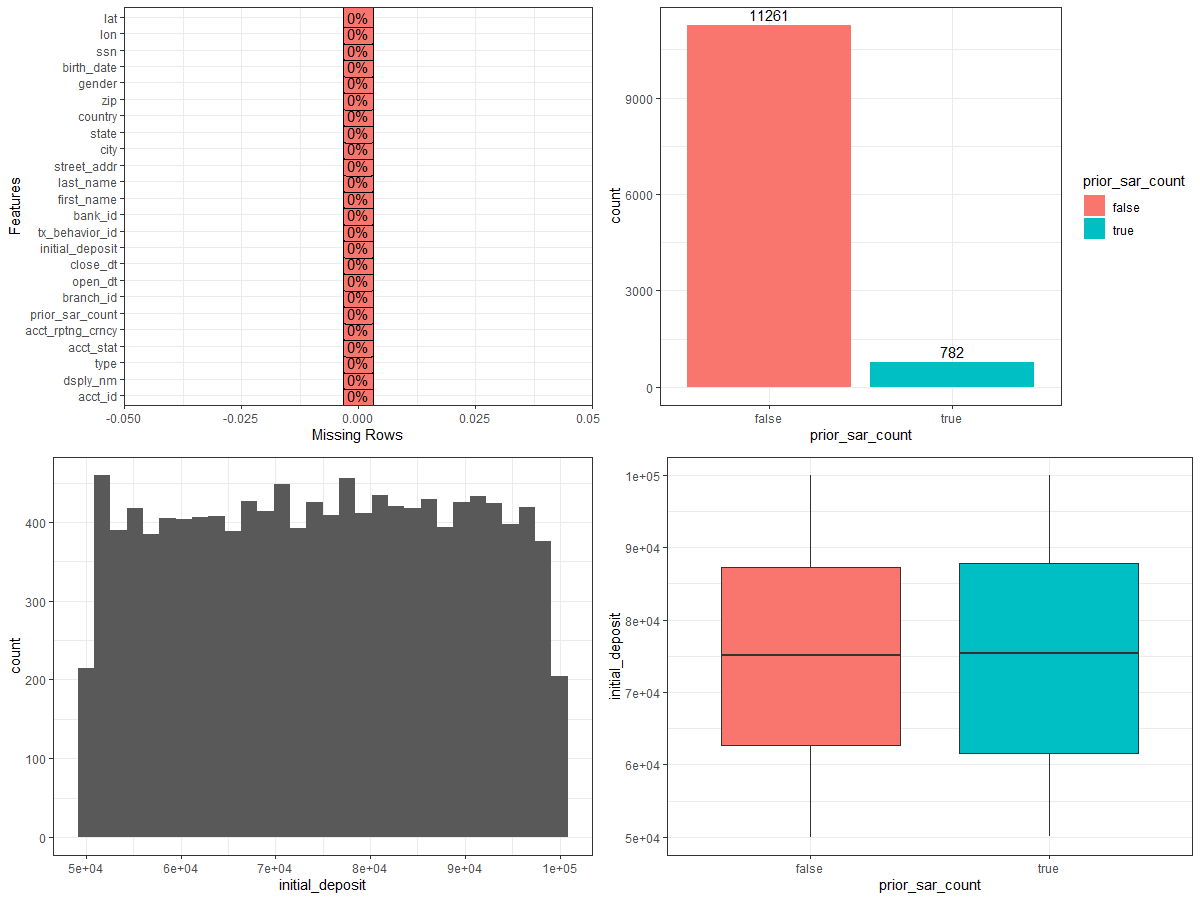
\includegraphics[scale=0.5]{fig/CH3/train_acc_summary.png}
		\caption{Example of the visualisations generated during the EDA of the training \texttt{accounts.csv} file. (top-left) The missing values profile. (top-right) Frequency bar chart of accounts that did and did not participate in money laundering activity. (bottom-left) Histogram of the accounts initial balances (\texttt{initial\_deposit}.  (bottom-right) A box and whiskers plot showing money laundering and honest accounts' initial deposits.}
		\label{fig:ch3_raw_eda_train_acct_sum}
	\end{center}	
\end{figure}

\section{Feature engineering} \label{ch3_sub_heading_feature_engineering}

%[Introduction to feature engineering section]
The previous section explained the raw data generation process (step one in Figure\ref{fig:ch1_project_framework}). This section  provides the details of the feature engineering process - how the raw data was used to create new features. The section will explain how each of the three structure data sets was constructed: \textit{network feature} data set, \textit{transactional feature} data set, and \textit{combined feature} data set. The previous section  mentioned that AMLSim was used to generate two raw data sets, a training data set and a testing data set. The feature engineering process for both data sets was identical. Therefore, both raw data sets will be referred to as the ``raw data set'' for this section.  
As mentioned in the previous section, the output of AMLSim is four raw data files. However, the project used only two of the files (\texttt{transactions.csv} and \texttt{accounts.csv}) for the feature engineering process. The finalised raw data, used as input for the feature engineering process, is displayed in Table\ref{tab:ch3_raw_data_final}. 

\begin{table}
\begin{tabular}{cll}
\hline
\multicolumn{1}{l}{\textbf{Raw data table}} & \textbf{Feature name} & \textbf{Description}                                                                                          \\ \hline
\multirow{3}{*}{\texttt{accounts.csv}}               & \texttt{acct\_id}              & ID number of client account.                                                                                  \\
                                            & \texttt{prior\_sar\_count}    & \begin{tabular}[c]{@{}l@{}}If the account has been involved in any money \\ laundering activity.\end{tabular} \\
                                            & \texttt{initial\_deposit}     & \begin{tabular}[c]{@{}l@{}}The initial balance when the client created \\ the account.\end{tabular}           \\ \hline
\multirow{7}{*}{\texttt{transactions.csv}}           & \texttt{tran\_id}              & ID number for transaction.                                                                                    \\
                                            & \texttt{origin\_acct}          & The account ID that makes the funds transfer.                                                                 \\
                                            & \texttt{bene\_acct}           & The account ID that receives the funds transfer.                                                              \\
                                            & \texttt{base\_amt}             & The transaction amount transferred.                                                                           \\
                                            & \texttt{tran\_timestamp}       & The date and time the transaction occured.                                                                    \\
                                            & \texttt{is\_sar}              & \begin{tabular}[c]{@{}l@{}}If the transaction is a money laundering \\ transaction.\end{tabular}              \\
                                            & \texttt{alert\_id}             & \begin{tabular}[c]{@{}l@{}}The ID indicating the type of money laundering \\ typology occurred.\end{tabular}  \\ \hline
\end{tabular}
\caption{The Table provides the finalised raw data tables used in the project (for both the testing and the training set). In addition, the table details the raw data table name, the features of the raw data table and a short description of each.}
\label{tab:ch3_raw_data_final}
\end{table}

%[Generation of Network feature data set - undirected weighted graph]
The network metrics chosen for the \textit{network feature data set} was the most popular network metrics applied for some anti-money laundering application found in literature \citep{boccaletti2006complex, zanin2016combining, colladon2017using, drezewski2015application, van2017gotcha}. \citet{baesens2015fraud} was specifically helpful in defining the network metrics. Also, they provided toy examples that the project used to validate and verify the output of the network extraction functions used to generate the network feature data set. The network feature data set was the first structured data set generated using the raw data. Firstly an undirected network was constructed using the raw data files. The vertices in the networks would represent the accounts, and the edges would represent the transactions made between accounts. Since an account can make (receive) multiple transactions to (from) another account, multiple edges exist in the network. Therefore, the network is a multigraph. Also, the network constructed did not contain any loops (accounts transferring money to themselves). Then the undirected network, containing multiple edges, was simplified to an \textit{undirected weighted network} by aggregating the transactions amounts between two vertices and collapsing the multiple edges between two nodes into a single edge. For example, $w_{AB}$ is calculated by:

$$\sum_{i = 1}^{k}TX(l_{AB})_i + \sum_{j=1}^{d}TX(l_{BA})$$

where $TX()$ is a function that extracts the transaction value of the $i^{th}$ or $j^{th}$ edge $l_{AB}$ or edge $l_{BA}$, respectively. Here, the values $k$ and $d$ represent the number of edges from node $A$ to $B$ and $B$ to $A$, respectively. Therefore, the weights between adjacent nodes represent  the total transactional amount exchanged between the nodes. Recall that a weight should be defined such that it serves as an indication of the strength of the relationship between neighbouring nodes. Therefore, the project assumed that nodes (accounts) with a high total transaction exchange amount exhibit a strong relationship. After the undirected weighted network was defined, it was divided into its graph components. It was decided to only consider graph components of size $N > 2$, due to graph components with size $N=1$ or $N=2$ producing \texttt{NA} and \texttt{Inf} values for multiple of the chosen network metrics (for example, transitivity, triangles, closeness centrality, etc.). Also, graph components of size $N<3$ seem to be either a client account recently opened (which made one or two transactions) or accounts that exhibit minimal financial activity (possibly a client that has other bank accounts). After extracting the graph components, the extraction of the network metrics could commence. Features 1-22 in Table \ref{tab:ch3_network_features} in appendix \ref{app_1} provides the list of all the network-related features extracted from each undirected weighted graph component and a short description of each. 

%[Generation of Network feature data set - directed graph]
After the network metric extraction from the undirected weighted graph components was complete, a \textit{directed network} was constructed using the raw data files. A directed network was constructed to extract useful network information concerning the \textit{direction} of transactions (which was not captured in the undirected weighted network). The process of extracting the network metrics from the directed graph was similar to the undirected weighted graph. After constructing the directed graph, the graph was divided into components of size $N>2$ (for the same reasons as mentioned before). Then for each graph component, its network metrics were extracted. Features 23-28 in Table \ref{tab:ch3_network_features} in appendix \ref{app_1} provides the list of all the network-related features extracted from each directed graph component and a short description of each. Finally, the network feature data set was constructed by joining the features extracted from the undirected weighted network and the directed network using the \texttt{acct\_id} as the primary joining key. Table \ref{tab:ch3_network_features} provides the finalised features for the network feature data set. 

%[Generation of transaction data set]
The generation of the \textit{transactional feature data set} was much more straightforward. The goal was to construct as many useful features from the raw data sets, that could provide a machine learning model with the right inputs to identify hidden patterns within the data. Therefore, the project applied no network analytic's to construct the transactional feature data set. \citet{visserdetection} also used the AMLSim simulator to generate data for anti-money laundering research purposes. However, their approach focused on using transactional-based features to predict illicit activity. Therefore, most  transactional features were derived from their work. Table \ref{tab:ch3_trans_features} in appendix \ref{app_1} provides the list and a description of all the transactional features generated for the transactional feature data set.      

%[Generation of combined data set and conclusion of section]
The final structured data set is the combined feature data set. This data set contains all the features generated during the feature engineering process. Therefore, the combined data set contains network features and transactional features. The combined feature data set can be visualised when the features from Tables \ref{tab:ch3_network_features} and \ref{tab:ch3_trans_features} are joined by using the \texttt{acct\_id} as the primary joining key.  

\section{Modelling} \label{ch3_sub_heading_modelling}

The previous section explained how all three structured data sets were constructed using the raw data (generated using AMLSim). To clarify, the project applied the feature engineering process for both the training and testing raw data sets. Therefore, there is a training and testing set for each data set (network feature data set, transactional feature data set, and combined feature data set). This section tests the project research hypothesis by using these structured data sets as input to two different classifiers. The first classification model will be a \textit{logistic regression} model, and the second classifier will be a \textit{neural network} model. The classification task is to predict, based on the given input features (network, transactional, or combined), if an account is participating in money laundering activity or not (the \texttt{is\_fraud} feature). A brief introduction to each classification model, the data pre-processing, hyper-parameter tuning and training, and evaluation of model performance are detailed in the section.               

% [Introduction - logistic regression]
Linear regression is a well established technique and has been studied for an extended period. While linear regression might seem like a monotonous method, compared to some modern-day statistical learning approaches, it remains an effective and extensively used statistical learning method \citep{james2013introduction}. For example, it can be argued that in the case where unknown target function $f$, is highly complex, a simple hypothesis set, $\mathcal{H}_{simple}$ would provide a better approximation $\hat{f}$, as to try to match the complexity of $f$, with a more complex hypothesis set $\mathcal{H}_{complex}$ \citep{abu2012learning}. Linear regression is a useful tool for predicting a quantitative response; however, the model can be easily extended to predict a qualitative response. This class of model is the \textit{logistic regression model}. The logistic regression model is more concerned with modelling the \textit{probability} that $y_i$ belongs to a certain class \citep{james2013introduction}. A short introduction to the logistic regression model follows. Suppose we have a binary classification problem with response:


$$y_i = \left \{\begin{array}{ll} 
 1 & \pi_i \geq \theta  \\ 
 0 & \pi_i < \theta  
\end{array} \right.
$$

where $\pi,\theta \in [0,1]$ and the threshold is assumed to be $\theta = 0.5$. If we would like to model the relationship between $\pi_i = Pr(y_i = True|\boldsymbol{x}_i)$ and $\boldsymbol{x}_i$ using the logistic regression model we need to start with the linear equation (as  \citet*{et2020analytics} explains):

$$\eta_i = \boldsymbol{x}_i^T\boldsymbol{w}$$

The idea is to define a ``link'' function, $h$, that maps $\eta \in \mathcal{R}$ to $[0,1]$. There are various choices for the function $h$. It can be the ``Logit'' function, ``Probit'' function, or complimentary log-log function. Suppose we use the ``Logit'' function as our ``link'' function, then the relationship between the linear component $\boldsymbol{x}_i^T\boldsymbol{w}$  and $\pi_i$ is expressed as:

$$\pi_i =  \frac{e^{\boldsymbol{x}_i^T\boldsymbol{w}}}{1 + e^{\boldsymbol{x}_i^T\boldsymbol{w}}}$$

Therefore, given the parameter vector $\boldsymbol{w}$ values, we may ``predict'' a probable result for a given set of features $\boldsymbol{x}_i$. To obtain suitable values for $\boldsymbol{w}$ we use the \textit{maximum likelihood} method. More specifically, we maximise the log-likelihood function:

\begin{equation}
    l(\boldsymbol{w}) = \sum_{i=1}^{n}(y_ilog(h^{-1}(\boldsymbol{x}_i^T\boldsymbol{w})) + (1-y_i)log(h^{-1}(\boldsymbol{x}_i^T\boldsymbol{w}))
\label{ch3_log_lik_eq}
\end{equation} 
 
After an suitable numerical optimisation routine is defined and a estimation of the weight parameter $\boldsymbol{\hat{w}}$ is defined, then the probability predictions are $\hat{\pi} = h(\boldsymbol{x}^T\hat{\boldsymbol{w}})$.

% [ Model definition - logistic regression]
Logistic regression models are capable of dealing with categorical predictors. Luckily, all three structured data sets had numerical predictors. Therefore, before any logistic regression models were implemented, the data pre-processing was to \textit{standardise} the data. Al three structured data sets were standardised since some of the features were not of the same unit of measure. Standardisation is recommended as an effective tool to solve this problem \citep{james2013introduction}. Furthermore, all logistic regression models were defined using the ``Logit'' function as the chosen ``link'' function. The optimisation routine or learning algorithm used to approximate a maximum for the log-likelihood function (Equation \ref{ch3_log_lik_eq}) was the Iterative Weighted Least Squares method (IWLS). This logistic regression model was applied to each structured training data set along with an L1 regularisation penalty. 

% [Regularisation - logistic regression]
Regularisation is a valuable technique for controlling a model's flexibility/complexity \citep{et2020analytics}. Managing the complexity of a model, using some regularisation mechanism, can also improve the models' ability to \textit{generalise} out of sample. Therefore, the model achieves a low in-sample error $E_{in}$ (typically the training error), but also a low out-of-sample error $E{_{out}}$ (typically the validation error). The only challenge in introducing some regularisation mechanism is the additional hyper-parameter(s) that must be ``tuned''. In applying \textit{L1 regularisation}, the only hyper-parameter that needs to be specified is the \textit{regularisation factor}, $\lambda$. In approximating the best $\lambda$ for each data set, the project used the process of \textit{K-fold-cross-validation}. Using $K = 10$ is an appropriate choice for the number of folds since it represents a suitable balance between unbiased estimation (leave-one-out cross-validation) with large variation and biased estimation with low variation but at the risk of overestimating the out-of-sample performance since a large portion of
the data is used to fit the model \citep{et2020analytics, friedman2001elements}. Figure \ref{fig:ch3_lr_lambda_cv_network} illustrates the ten-fold cross-validation applied to the logistic regression models with the L1 penalty for the network feature data set. The identical plots for the transactional feature data set and combined feature data set are illustrated in Appendix \ref{app_1} Figure \ref{fig:ch3_lr_lambda_cv_trans} and Figure \ref{fig:ch3_lr_lambda_cv_all}, respectively. Also, there are two vertical dashed lines in the plots mentioned above. The first line (from the left) indicates $\lambda_{min}$. At this $\lambda$ value, the MSE is at its minimum. The second line indicates $\lambda_{1 SE}$ which is the biggest $\lambda$ value that is one standard error from the $\lambda_{min}$. The $\lambda_{1 SE}$ was the chosen regularisation factor value for all logistic regression models, which had L1 regularisation applied. This decision was made because the regularised model with the higher regularisation factor ($\lambda_{1 SE}$) is, the more ``penalised'' model and, therefore, less complex. The simplest model that delivers similar performance to the best model is often the better choice \citep{friedman2001elements}.      

% [Threshold selection - logistic regression]
The \textit{threshold value} ($\theta$) was briefly mentioned in the introduction of the logistic regression model. The value of the threshold parameter determines the mapping from the predicted probability value, $\hat{\pi_i}$ to the respective class. For most classification problems, the default value for the threshold is 0.5. However, if the classification problem has \textit{high class imbalances}, such as in the project, then the default threshold can produce poor classification performance \citep*{jason2016brownlee}. Therefore the project used two methods in determining the threshold value for each logistic regression model defined. The first method was finding the optimal threshold according to the \textit{Receiver Operating Characteristic} curve (ROC). In short, the ROC curve plots a models performance for a range of threshold values where the false-positive rate ($FPR$) is shown on the x-axis and the true-positive rate ($TPR$) is shown on the y-axis. The optimal threshold value, according to the ROC curve, is the threshold value that produces the maximum \textit{Geometric Mean} ($G_{mean}$). The G-mean is calculated by: $G_{mean} = \sqrt{TPR\times(1-FPR)}$. This point on the ROC curve is usually found in the upper left side of the curve. The second method was finding the optimal threshold value according to the \textit{precision-recall curve}. In short, \textit{precision} ($p_r$) is the ratio of the number of true positives divided by the sum of the true positives, and false positives and \textit{recall} ($r_c$) is the ratio of the number of true positives divided by the sum of the true positives and the false negatives. Similarly to the ROC curve, the precision-recall curve plots a models performance for a range of threshold values where the recall is shown on the x-axis and the precision is shown on the y-axis. The optimal threshold value, according to the precision-recall curve, is found at the threshold value where the \textit{F-measure} or \textit{F1-score} ($F_1$) is at its maximum. Equation \ref{ch3_f1_eq} shows how the F1-score is calculated. Figure \ref{fig:ch3_lr_thresh_roc_lasso_network} and Figure \ref{fig:ch3_lr_thresh_pr_lasso_network}illustrate the optimal threshold value chosen according to the ROC curve and precision-recall curves for the logistic regression model with an L1 penalty applied to the network training data.  

  % 10-Fold cross-validation (lambda - network data)
\begin{figure}
	\begin{center}
		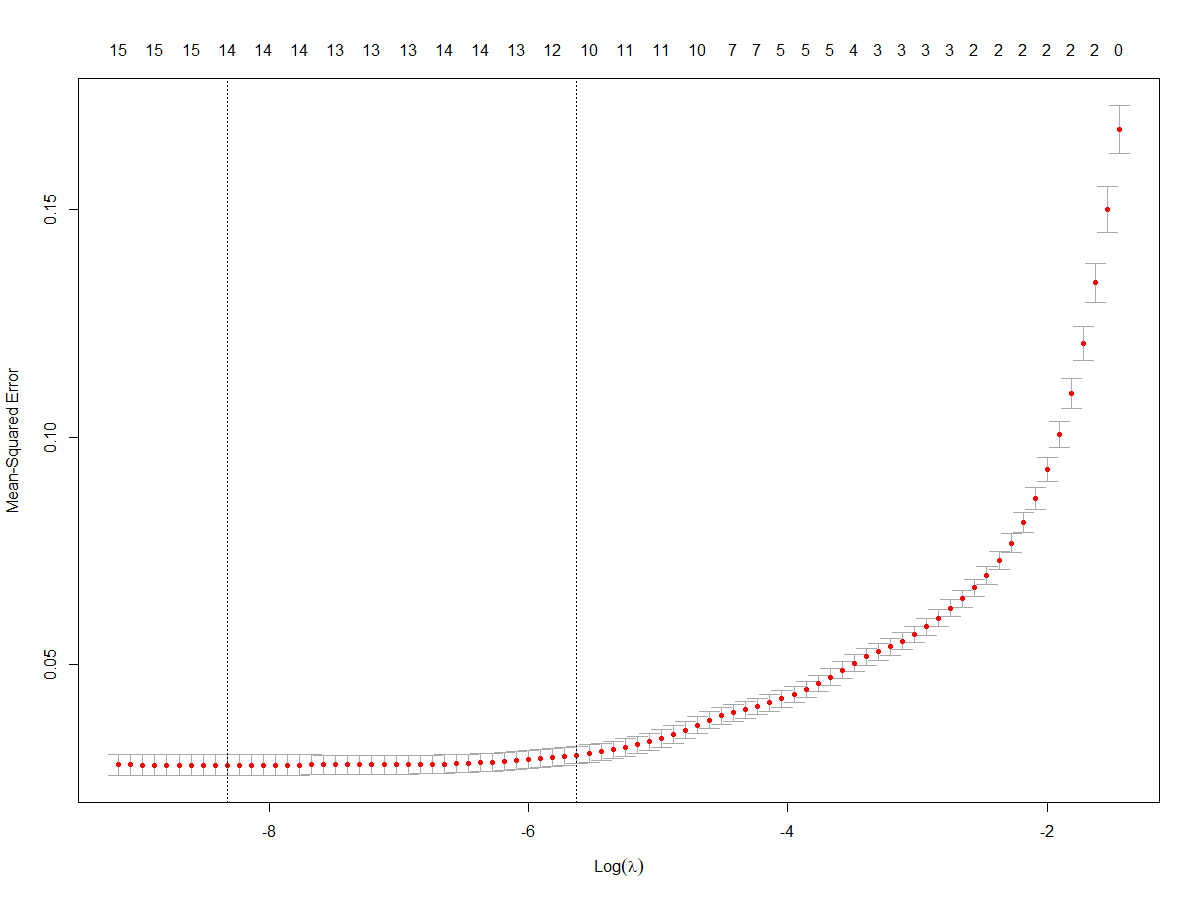
\includegraphics[scale=0.45]{fig/CH3/cv_lambda_network.png}
		\caption{Ten-fold cross-validation mean square error (MSE) for the L1 regularised logistic regression model applied to the network feature data set. The vertical dashed line on the left is the $log(\lambda)$ value of where the MSE is at its minimum and the vertical on the right is the largest $log(\lambda)$ value such that the MSE is within one standard error of the minimum MSE. Also, the plot illustrates at the top, the number of positive weights $\boldsymbol{w} > 0$ at a specific $log(\lambda)$ value.}
		\label{fig:ch3_lr_lambda_cv_network}
	\end{center}	
\end{figure}

% Threshold moving - ROC LR lasso network data
\begin{figure}
	\begin{center}
		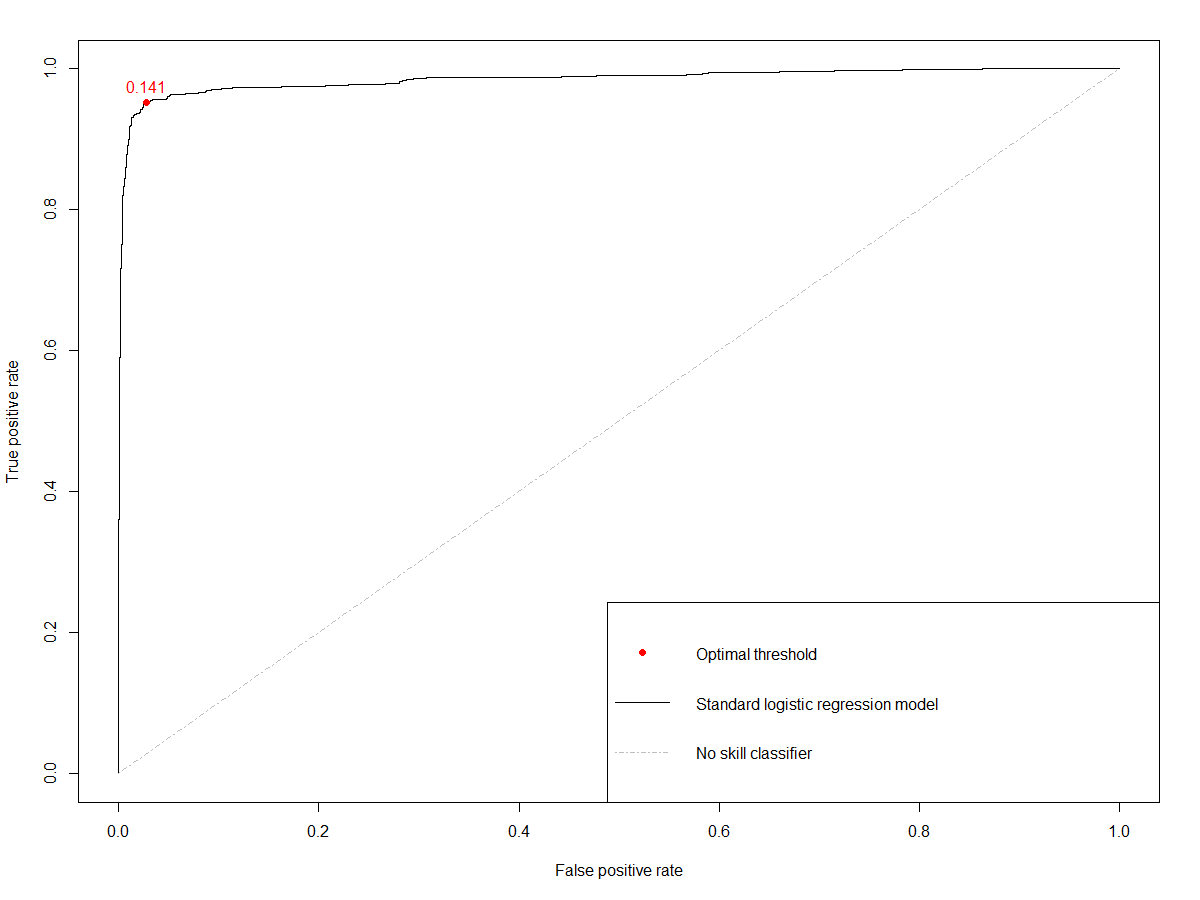
\includegraphics[scale=0.45]{fig/CH3/lasso_log_ROC_threshold_network.png}
		\caption{The ROC curve of the logistic regression model with an L1 penalty applied to the training network feature data set. Also, the plot provides the optimal threshold point (the threshold value that maximised the Geometric mean).}
		\label{fig:ch3_lr_thresh_roc_lasso_network}
	\end{center}	
\end{figure}

% Threshold moving - PR LR lasso network data
\begin{figure}
	\begin{center}
		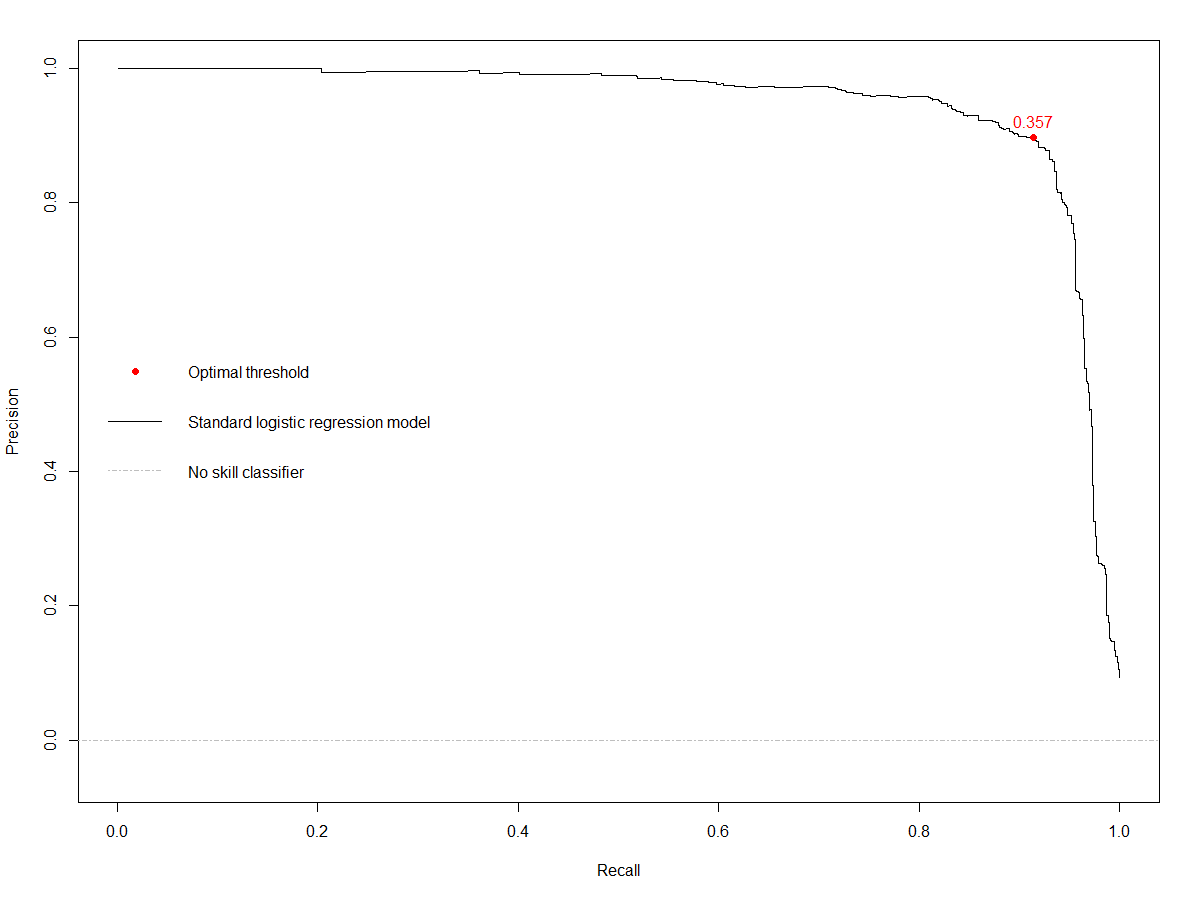
\includegraphics[scale=0.45]{fig/CH3/lasso_log_PR_threshold_network.png}
		\caption{The precision-recall curve of the logistic regression model with an L1 penalty applied to the training network feature data set. Also, the plot provides the optimal threshold point (the threshold value that maximised the F-measure).}
		\label{fig:ch3_lr_thresh_pr_lasso_network}
	\end{center}	
\end{figure}

% Neural networks
The second classifier is a \textit{ neural network}. The neural network model is a class of non-linear models used in supervised learning tasks \citep{et2020analytics}. Literature commonly compares the neural network model to that of the human brain. Although some terminology may overlap, one should not confuse its functioning with a biological neural network. As \citet{et2020analytics} said, the neural network is simply a mathematical model based on the idea that by the repeated iteration of translations of the input (with the depth of the network providing the number of repetitions) and specification of the calculation performed in each cell (node), we create a non-linear function of the input/predictor space which maps to the output. A more formal definition of a neural network, specifically a standard \textit{feed-forward neural network}, is as follows (adopted from \citep{et2020analytics}:

Let $a^l_j$ denote the $j^{th}$ node on $l^{th}$ layer of a standard feed-forward neural network, then the network structure can be written as an updating equation (in vector form):

$$\boldsymbol{a}^l = \sigma_l(\boldsymbol{W^T_l}\boldsymbol{a}^{l-1}+\boldsymbol{b}^l);\; l = 1,2,\ldots$$

where  $\boldsymbol{a}^l = [a^l_1,a^l_1,\ldots,a^l_j]^T$ denote vectors of activations. The parameters of the model are summarised in the weight matrices $\boldsymbol{W_l} = (w^l_{kj})$, where $w^l_{kj}$ is the $kj$-th weight paramter linking the $k$-th node in layer $l-1$ and $j$-th node in layer $l$. The bias vectors are denoted by $\boldsymbol{b}^l = [b^l_1,b^l_2,\ldots,b^l_j]^T$, and the initial values(s) for the equation is $\boldsymbol{a}^0 = \boldsymbol{x}_i$. Lastly, the $\sigma(.)_l$ denotes the activation function on layer $l$.

The above equation has the potential to emulate highly non-linear functions in the predictors. Also, increasing the number of nodes or layers within the equation increases the number of model parameters, and as a result, increases the models' complexity. As with the logistic regression model, in which the Equation \ref{ch3_log_lik_eq} needed to be maximised to obtain suitable weights for the model, so too does a neural network model need some optimisation technique to estimate appropriate weights within $\boldsymbol{W_l}$. \textit{Gradient descent} (or variants thereof) combined with \textit{backpropagation} is used to fit neural networks. Gradient descent is a numerical technique for finding extrema (such as Newton's method). The fundamental idea behind gradient descent is for each iteration, the algorithm tries to ``step'', with a certain \textit{magnitude}, in the \textit{direction} that improves the cost function. Both the direction and magnitude of the step-size are based on the cost function gradient given a set of inputs. On the other hand, backpropagation is an algorithm for calculating the gradient of a cost function with respect to variables of a model. Therefore, during the neural networks' training, the gradient for each weight in the network is calculated using backpropagation. After that, gradient descent uses the gradient to update the models' weights. The project will not provide the mathematical formulations of gradient descent and backpropagation; however, \citet*{nielsen2015neural} gives a thorough explanation of each.

Unlike the logistic regression model, the neural network model can not take categorical features as inputs. The neural networks can only take numerical predictors. As mentioned before, luckily, this is not a problem since all three structured data sets had numerical predictors. Standardising the predictor variables was the only data pre-processing necessary. This data pre-processing step was done due to the predictors' different units of measures. It is highly recommended that before implementing any neural network, one should ensure the same scales across all input variables \citep*{bishop1995neural}. The project defined two different neural networks in the project. Both models were standard feed-forward neural networks with a \textit{single} hidden layer. Based on the networks architecture, the only difference was the \textit{number of nodes} defined in the hidden layer. The first model had 8 hidden neurons and the second model had 64 hidden neurons. Architecturally, the number of hidden nodes in the hidden layer was the only difference. The activation function applied in the hidden layer and output layer of the models were the \textit{rectified linear unit} (ReLU) and \textit{soft-max} activation functions. The ReLU activation  function is a very popular activation function to use within hidden layers. ReLU's piecewise linear function provides a lot of desirable properties of a linear function when training a neural network using backpropagation \citep*{goodfellow2017deep}. However, the choice of the hidden layer activation function for neural networks becomes more significant when the depth of the network increases tremendously (as with \textit{deep learning} models) \citep{et2020analytics}. Therefore, the ReLU activation function will be sufficient for the hidden layers of the project neural network models. In terms of the activation function used in the output layer, we need to choose an activation function that matches the range of the encoded outputs due to the problem being a classification task \citep{et2020analytics}. It is useful to ensure that the output layer behaves like a \textit{distribution}, and therefore, the soft-max activation function was chosen. The cost function defined in training the neural networks was the so-called \textit{cross-entropy error}. This cost function is desirable since the gradient of the cross-entropy function w.r.t the model's parameters are less likely to ``bottoming out'' when it's far from a global solution \citep{et2020analytics}. The chosen optimiser used for each model was the \textit{adam} optimiser. The adam optimiser is an extension of the stochastic gradient descent learning algorithm, which takes as input three hyper-parameters: \textit{batch size}, \textit{epochs}, and  \textit{learning rate} $\nu$. There is no defined process in choosing the batch size or training epochs \citep{bengio2012practical, masters2018revisiting}. Choosing large batch sizes provides the learning algorithm with more training examples, which provides a more accurate estimate of the cost functions error gradient. Therefore, it is more likely that the weights of the network will be adjusted correctly so that the performance of the model increases. The drawback of choosing a large batch size (like in batch size gradient decent) is that the cost functions error gradient becomes highly dependent on the training samples used (which can negatively impact the model's generalisation). Alternatively, using small batch sizes results in less accurate estimates of the error gradient, which provides a ``noisy'' update to the weights. These noisy updates can result in faster learning and sometimes more robust models \citep*{jason2019batch}. On the other hand, the training epochs is the number of full pass overs of the training dataset. A small number of epochs is computationally beneficial, however, you run the risk of the algorithm not completely reaching an extremum. Depending on the problem, choosing a very high number of training epochs is also not ideal since it can lead to overfitting the model. This begin said the batch size and epoch values chosen for both models were 100 and 20, respectively. Also, 0.001 was chosen as the \textit{learning rate} for the adam optimiser (the optimisers default value).

As mentioned before, regularisation is a useful technique in controlling a models complexity. Some of the most straightforward neural network architectures are able to construct complex non-linear functions. Therefore, it is essential to apply some form of regularisation mechanism, in which we can ensure that our model has generalised to some degree. \textit{L2 regularisation} was the chosen regularisation method for the neural network models. As mentioned with the logistic regression model, the implication of adopting L2 regularisation is that an additional hyper-parameter, $\lambda$, needs to be specified. The project determined an appropriate value for $\lambda$ each neural network model by using a validation set (hold-out set). Therefore, 70\% was used for training (fitting) the models for each structured training data set, and 30\% was used for validation. Figure \ref{fig:ch3_nn_validation_mod1_network} and Figure \ref{fig:ch3_nn_validation_mod2_network}  illustrate the process of finding the best approximate $\lambda$ value for the (8)-network and (64)-network, respectively, using the network feature data set. Two plots are shown in the Figure. The left plot shows the validation and training errors for $\lambda \in [0,1]$. The right plot also shows the validation and training errors but for a more focused set of $\lambda$ values. Also, the value of $\lambda$, which produced a minimum validation error, is shown by the red dashed line. This type plot was constructed for each of the two neural network models (the (64)-network and the (8)-network) for each structured training data set (network feature, transactional feature, and combined.). In appendix \ref{app_2} Figures \ref{fig:ch3_nn_validation_mod1_trans} and \ref{fig:ch3_nn_validation_mod2_trans} show the best approximated $\lambda$ values for the transactional feature data set for the (8)-network and (64)-network models, respectively. Also, Figures \ref{fig:ch3_nn_validation_mod1_all} and \ref{fig:ch3_nn_validation_mod2_all} show the best approximated $\lambda$ values for the combined feature data set for the (8)-network and (64)-network models, respectively.

% [conclusion - modelling]
This section explained the modelling procedure implemented in the project. For both the logistic regression and neural network models: the data pre-processing was done, the models' architectures were defined, and hyper-parameter tuning was performed to find appropriate values for the models hyper-parameters. The final step in the modelling procedure was choosing which models would most likely deliver good out-of-sample performance based on the training results. The out-of-sample performance of the model will be estimated using test data sets (``unseen'' data sets). Three models were chosen to be evaluated against the test data sets (test network feature data set, test transactional feature data set, and test combined feature data set). The first model was the logistic regression model with L1 regularisation. The threshold value chosen for the model was based on the optimal threshold according to its ROC curve. The second model was identical to the first. However, the threshold value was chosen according to the optimal threshold value calculated from its precision-recall curve. The final model was the (8)-network model. The (8)-network model was preferred over the (64)-model because both yielded similar validation errors for each structured data set. Figure \ref{fig:ch3_nn_validation_compare_network} illustrates this point for the network feature data set. Figure \ref{fig:ch3_nn_validation_compare_trans} and Figure \ref{fig:ch3_nn_validation_compare_combined} in appendix \ref{app_1} show a similar result. Therefore, as \citet{james2013introduction} recommends, it is better to choose the simpler model that delivers a similar performance to the complex model. From here onwards, the project will refer to the first model as ``LR-ROC'', the second model as ``LR-PR'' and the third model as ``(8)-NN''. Also, Table \ref{tab:ch3_model_summary} provides a summary of the three models and how they were configured for each data set. The results, after testing the models on the test data sets, are presented in section \ref{ch3_sub_heading_results}.

% validation curves NN -  (8)-network data
\begin{figure}
	\begin{center}
		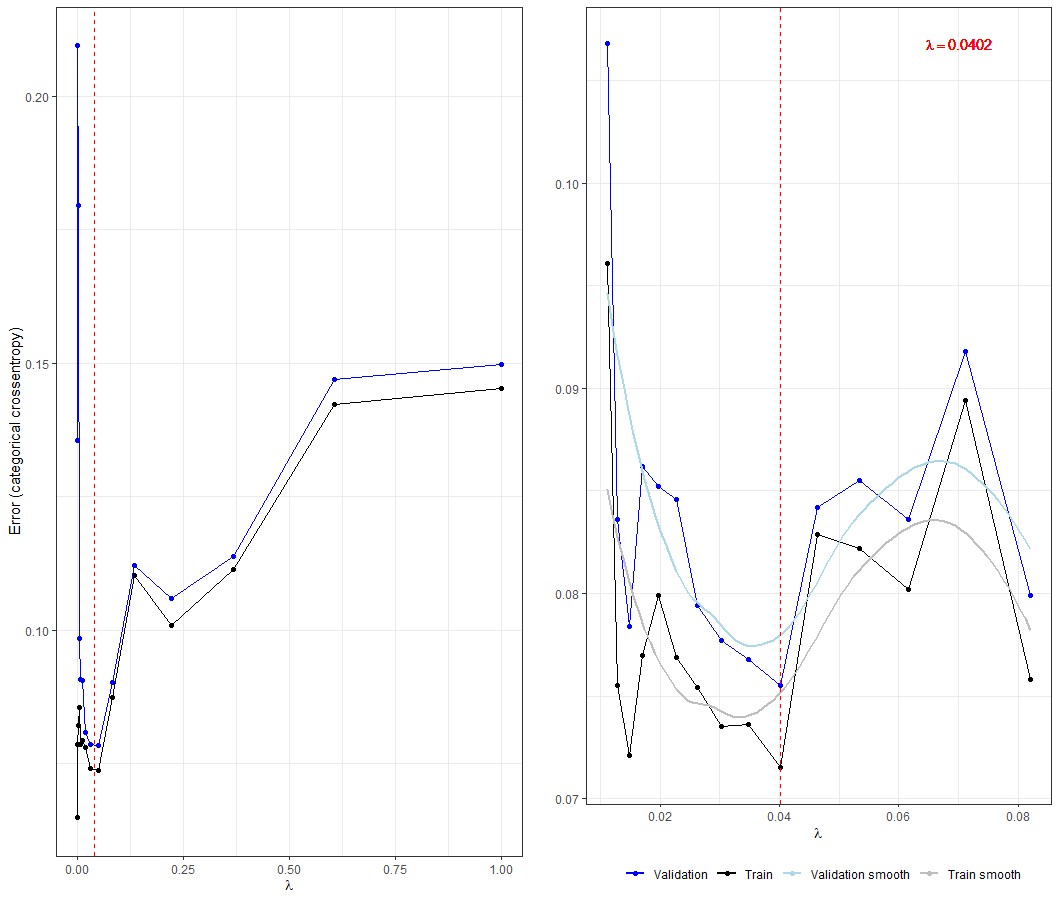
\includegraphics[scale = 0.55]{fig/CH3/network_mod_1_lambda_plot.png}
		\caption{The plot illustrates the process of selecting the best approximate $\lambda$ value for the (8)-network model applied to the network feature data set. (left) The training and validation set errors for a range of $\lambda$ values. (right) The training and validation set errors for a more specific range of $\lambda$ values. The training and validation error smooth curves are auxiliary curves to help view the curve patterns. Also, the $\lambda$ value that produced the minimum validation error is shown in both plots.}
		\label{fig:ch3_nn_validation_mod1_network}
	\end{center}	
\end{figure}

% validation curves NN -  (64)-network data
\begin{figure}
	\begin{center}
		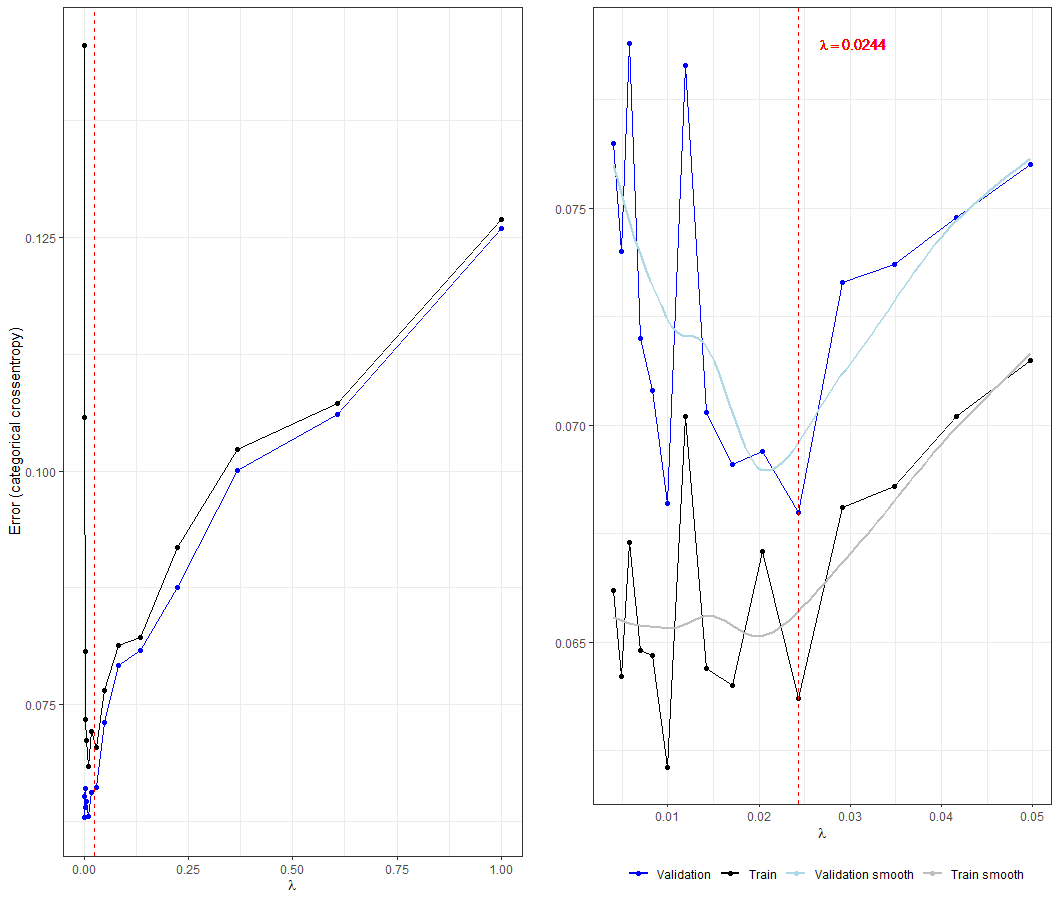
\includegraphics[scale = 0.5]{fig/CH3/network_mod_2_lambda_plot.png}
		\caption{The plot illustrates the process of selecting the best approximate $\lambda$ value for the (64)-network model applied to the network feature data set. (left) The training and validation set errors for a range of $\lambda$ values. (right) The training and validation set errors for a more specific range of $\lambda$ values. The training and validation error smooth curves are auxiliary curves to help view the curve patterns. Also, the $\lambda$ value that produced the minimum validation error is shown in both plots.}
		\label{fig:ch3_nn_validation_mod2_network}
	\end{center}	
\end{figure}

% validation curves comparison NN -  network data
\begin{figure}
	\begin{center}
		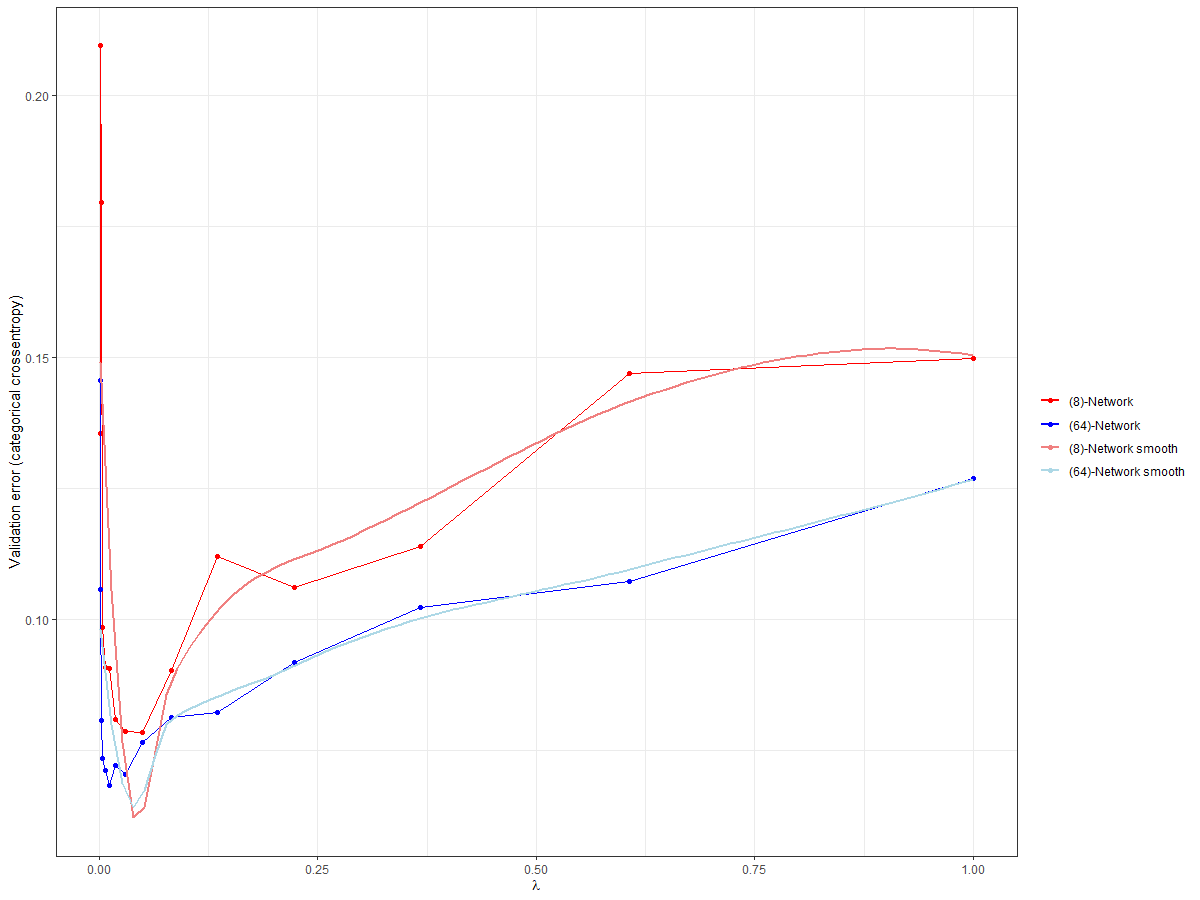
\includegraphics[scale = 0.5]{fig/CH3/model_comp_network_HL.png}
		\caption{The superimposed validation error curves of the (8)-Network and (64)-Network models and their smoothing curves for $\lambda \in [0,1]$. Both models were applied to the network features data set.}
		\label{fig:ch3_nn_validation_compare_network}
	\end{center}	
\end{figure}

% model summary table
\begin{table}
\resizebox{\columnwidth}{!}{%
\begin{tabular}{llclll}
\hline
\multicolumn{1}{c}{\textbf{\begin{tabular}[c]{@{}c@{}}Model \\ name\end{tabular}}} & \multicolumn{1}{c}{\textbf{\begin{tabular}[c]{@{}c@{}}Model \\ type\end{tabular}}} & \textbf{\begin{tabular}[c]{@{}c@{}}Regularisation \\ mechanism\end{tabular}} & \multicolumn{1}{c}{\textbf{\begin{tabular}[c]{@{}c@{}}Regularisation\\ factor\end{tabular}}}                                               & \multicolumn{1}{c}{\textbf{\begin{tabular}[c]{@{}c@{}}Additional \\ hyper-paramters\end{tabular}}}                                    & \multicolumn{1}{c}{\textbf{\begin{tabular}[c]{@{}c@{}}Additional \\ info\end{tabular}}}                                                                                                                                                                                                                                \\ \hline
LR-ROC                                                                             & \begin{tabular}[c]{@{}l@{}}Logistic \\ regression\end{tabular}                     & L1                                                                           & \begin{tabular}[c]{@{}l@{}}$\lambda_{network} = 0.003$;\\ $\lambda_{transactional} = 0.0003$;\\ $\lambda_{combined} = 0.0002$\end{tabular} & \begin{tabular}[c]{@{}l@{}}$\theta_{network} = 0.141$;\\ $\theta_{transactional} = 0.088$;\\ $\theta_{combined} = 0.159$\end{tabular} & \begin{tabular}[c]{@{}l@{}}The threshold was chosen according \\ to the optimal threshold on the ROC \\ curve.\end{tabular}                                                                                                                                                                                            \\ \hline
LR-PR                                                                              & \begin{tabular}[c]{@{}l@{}}Logistic \\ regression\end{tabular}                     & L1                                                                           & \begin{tabular}[c]{@{}l@{}}$\lambda_{network} = 0.003$;\\ $\lambda_{transactional} = 0.0003$;\\ $\lambda_{combined} = 0.0002$\end{tabular} & \begin{tabular}[c]{@{}l@{}}$\theta_{network} = 0.357$;\\ $\theta_{transactional} = 0.397$;\\ $\theta_{combined} = 0.462$\end{tabular} & \begin{tabular}[c]{@{}l@{}}The threshold was chosen according \\ to the optimal threshold on the \\ precision-recall curve.\end{tabular}                                                                                                                                                                               \\ \hline
(8)-NN                                                                        & \begin{tabular}[c]{@{}l@{}}Neural \\ Network\end{tabular}                          & L2                                                                           & \begin{tabular}[c]{@{}l@{}}$\lambda_{network} = 0.04$;\\ $\lambda_{transactional} = 0.002$;\\ $\lambda_{combined} = 0.03$;\end{tabular}    & \begin{tabular}[c]{@{}l@{}}Epochs = 20;\\ Batch size = 100;\\ $\nu$ = 0.001\end{tabular}                                              & \begin{tabular}[c]{@{}l@{}}Standard feed-forward neural network \\ with one hidden layer. The ReLU \\ activation function was applied in \\ the hidden layer and the soft-max\\ activation function was applied to \\ the output layer. Lastly, the  Adam \\ optimiser was used in training \\ the model.\end{tabular} \\ \hline
\end{tabular}
}
\caption{The Table provides a complete summary of the chosen models used to make predictions on each test data set. In addition, the hyper-parameters for each data set are also specified. Note that if the subscripts of the specific data set are not mentioned, then the specific hyper-parameter was kept the same for each data set.}
\label{tab:ch3_model_summary}
\end{table}

\section{Results}\label{ch3_sub_heading_results}

% Introduction to results section
The previous section explained the modelling procedure and how each model type was configured and constructed. Finally, the section concluded that three models (LR-ROC, LR-PR, and (8)-NN) were chosen to make predictions on unseen data. So far, the project has established an idea of each of the model's in-sample performance. However, this section aims to provide how the models performed out-of-sample.

% Introduction to the performances metrics used 
 The performance measures or metrics used to evaluate each data set's models were \textit{F1-score}, \textit{balanced accuracy}, and \textit{classification accuracy}. Although classification accuracy was included in the list of performance metrics, it is not an ideal classification performance metric if a data set is highly imbalanced \citep*{branco2015survey}. As mentioned before, approximately 1\% of all transactions are fraudulent, and approximately 5\% of all accounts have participated in money laundering activity. Therefore, the class distributions of the projects data sets are severely skewed. In such a case, the classification accuracy can be misleading due to the \textit{accuracy paradox} \citep{branco2015survey}. This phenomenon can be explained at the hand of the following toy example. Suppose we have a data set with a 1:100 class imbalance, ``0'' representing the majority class and ``1'' representing the minority class. If a naive model predicts ``0'' for all observations in the test set, then the model would have attained a classification accuracy of 99\%. On the surface, this seems like a very impressive result. However, one can easily forget that the naive classifier predicted only the majority class. This raises the question of whether the model's performance is as impressive as the classification accuracy depicts. In the example, the classification accuracy is correct. However, it is the analyst intuition, thinking the model actually ``learnt'', which is the real pitfall. 
 
% f1 - performance metric
Therefore, it is essential to define other performance metrics that can better cope with imbalanced data set such as the F1-score and balanced accuracy. The F1-score ($F_1$) is calculated as follows:

\begin{equation}
    F_1 = \frac{2 \times TP}{2 \times TP + FP + FN}
\label{ch3_f1_eq}
\end{equation} 

Where $FP$ is the false-positives - honest accounts predicted as fraudulent accounts, $TP$ is the true-positives - correctly predicted money laundering accounts, and $FN$ is the false-negatives - a money laundering account predicted as an honest account. The F1-score is also defined of as the harmonic mean of $precision = \frac{TP}{TP+FP}$ and $recall = \frac{TP}{TP + FN}$ \citep{james2013introduction}. Precision and recall are not much affected by heavily skewed data (as seen by their expressions). Therefore, the F1-score should be an appropriate performance metric since it combines precision and recall values into a single metric. On the other hand, balanced accuracy is calculated as follows:

$$Balanced\;accuracy = \frac{\frac{TP}{T_{P}} = \frac{TN}{T_{N}}}{2} $$

% balanced acc - performance metric
Where $T_{P}$ is the total positives and $T_{N}$ is the total negatives. By taking the average of the total number of positive cases correctly predicted ($sensitivity = recall$) and the total number of negative cases correctly predicted ($specificity = \frac{TN}{T_{N}}$), we are left with a measure illustrating the prediction performance of \textit{both} classes. For example, if we consider a naive binary classifier that only predicts the majority class (``0''), we will obtain a high value for specificity, however, it will obtain a very low value for sensitivity (representing the prediction accuracy of the minority class ``1'') resulting in a lower overall average between the two metrics. 
% results interpreation
Table \ref{tab:ch3_model_results} provides a summary of each models performance on each test data set. Classification accuracy was included; however one should be cautious when jumping to conclusions using this metric due to the aforementioned reasons. It is also important that note that a naive classifier, which only predicts the majority class (\texttt{is\_fraud} = False), would have obtained a classification accuracy of \textbf{94.5\%} on each test set. Models that received their inputs from the network feature data set will be referred to as the ``network feature models''. The same applies to the transactions and combined feature data sets. Starting with the F1-score metric, on average, the network feature models scored \textbf{0.371} higher than the transactional feature models. The combined feature models average F1-score performance was slightly better (0.01) than the average F1-score of the network feature models. Generally, the (8)-NN model delivered the highest F1-scores, however, on average, the LR-PR model was the better model. Looking at the balanced accuracy measurement, very high values were recorded for the network feature models. It was unexpected that each network feature model outperformed each respective combined feature model i.t.o balanced accuracy. On average, the transactional feature models scored much lower (\textbf{0.21}) than the network feature models. Overall, the two logistic regression models, LR-ROC and LR-PR, outperformed the (8)-NN model on balanced accuracy scores. Specifically, on average, the LR-ROC model outperformed the other models on the balanced accuracy metric. The defined model metrics help analyse the performance of each model, given the different set of input features. However, looking at each models \textit{confusion matrix} can also provide insight into the models' performance. The confusion matrices for all models for each data set is provided in appendix \ref{app_1}. Some noticeable findings were that all the network feature models (Tables \ref{tab:ch3_cm_LR_ROC_network}, \ref{tab:ch3_cm_LR_PR_network}, and \ref{tab:ch3_cm_nn_network}) had a relatively low number of false negatives. On the other hand, the transactional feature models had higher false positives (Table \ref{tab:ch3_cm_LR_PR_trans} and Table \ref{tab:ch3_cm_LR_PR_network}) and higher false negatives (Table \ref{tab:ch3_cm_LR_ROC_trans}). The confusion matrices of the combined feature models were very similar to the network feature models. From a practical point of view, it would be valuable for a commercial bank to pay close attention to the false positive accounts since these accounts seem to exhibit similar behaviour to the money laundering accounts and, therefore, are a higher risk.  

Finally, Figure \ref{fig:ch3_final_results_bar}, Figure \ref{fig:ch3_final_results_f1_density}, and Figure \ref{fig:ch3_final_results_balanced_acc_density} were included as visual illustrations of the results displayed in Table \ref{tab:ch3_model_results}. Looking at Figure \ref{fig:ch3_final_results_f1_density} and Figure \ref{fig:ch3_final_results_balanced_acc_density} it is very noticeable that the the network feature models performed much better i.t.o F1-score and balanced accuracy than the transnational feature models. The combined feature models scored slightly better than the network feature models in F1-score. Even though the network feature models obtained higher balanced accuracy scores than the combined feature models, the balanced accuracy distribution of the combined feature models was much narrower than that of the network feature models.  

% Model/Data set final results
\begin{table}
\begin{tabular}{cllll|l}
\hline
\textbf{\begin{tabular}[c]{@{}c@{}}Performance \\ metric\end{tabular}}        & \multicolumn{1}{c}{\textbf{\begin{tabular}[c]{@{}c@{}}Data \\ set\end{tabular}}} & \multicolumn{1}{c}{\textbf{LR-ROC}} & \multicolumn{1}{c}{\textbf{LR-PR}} & \multicolumn{1}{c|}{\textbf{(8)-NN}} & \multicolumn{1}{c}{\textbf{Average}} \\ \hline
\multirow{3}{*}{Accuracy}                                                     & Network feature                                                                  & 0.955                               & 0.978                              & $0.986^*$                            & 0.973                                \\
                                                                              & Transactional feature                                                            & 0.846                               & $0.95^*$                           & 0.935                                & 0.91                                 \\
                                                                              & Combined                                                                         & 0.953                               & 0.95                               & $0.988^*$                            & 0.964                                \\ \hline
\multicolumn{1}{l}{}                                                          & \textbf{Average:}                                                                & 0.918                               & 0.959                              & 0.97                                 &                                      \\ \hline
\multirow{3}{*}{F1-score}                                                     & Network feature                                                                  & 0.701                               & 0.826                              & $0.885^*$                            & 0.804                                \\
                                                                              & Transactional feature                                                            & 0.361                               & $0.577^*$                          & 0.361                                & 0.433                                \\
                                                                              & Combined                                                                         & 0.693                               & 0.857                              & $0.892^*$                            & 0.814                                \\ \hline
\multicolumn{1}{l}{}                                                          & \textbf{Average:}                                                                & 0.585                               & 0.753                              & 0.713                                &                                      \\ \hline
\multirow{3}{*}{\begin{tabular}[c]{@{}c@{}}Balanced \\ accuracy\end{tabular}} & Network feature                                                                  & 0.957                               & 0.969                              & $0.973^*$                            & 0.966                                \\
                                                                              & Transactional feature                                                            & $0.82^*$                            & 0.797                              & 0.652                                & 0.756                                \\
                                                                              & Combined                                                                         & $0.956^*$                           & 0.952                              & 0.954                                & 0.954                                \\ \hline
\multicolumn{1}{l}{}                                                          & \textbf{Average:}                                                                & 0.911                               & 0.906                              & 0.86                                 &                                      \\ \hline
\end{tabular}
\caption{A summary of the models (LR-ROC, LR-PR, and (8)-NN) results when applied to each test data set (network feature, transactional, and combined). The performance evaluation metrics were classification accuracy, F1-score, and Balanced accuracy metrics. The model that performed the best for a specific data set was indicated using the asterisk symbol ($*$). The average performance is shown on each data set's far most right column. In addition, the average performance for each model is shown in the rows between the metrics.}
\label{tab:ch3_model_results}
\end{table}

% Summary result figures - bar
\begin{figure}
	\begin{center}
		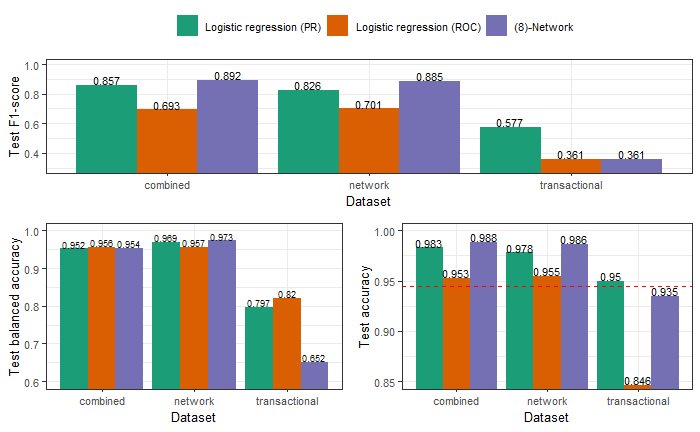
\includegraphics[scale = 0.8]{fig/CH3/data_sets_summary_bar.png}
		\caption{The plot shows a visual representation summarising the performance of each of the models on each test data set. (top) The F1-score for each model applied to each test data set. (bottom-left) The balanced accuracy score for each model applied to each test data set. (bottom-right) The classification accuracy for each model applied to each test data set. Also, the red dashed line indicates the classification accuracy of a naive classifier, which only predicted the majority class.}
		\label{fig:ch3_final_results_bar}
	\end{center}	
\end{figure}

% Summary result figures - density f1
\begin{figure}
	\begin{center}
		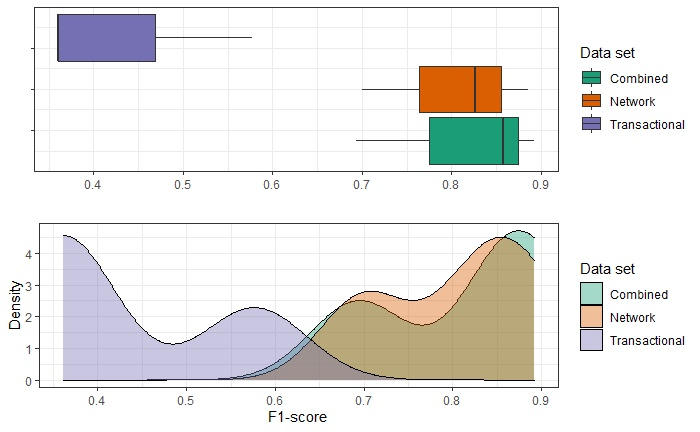
\includegraphics[scale = 0.6]{fig/CH3/data_sets_test_f1_density_LI.jpg}
		\caption{A visual representation of the tested models F1-score distribution grouped by the given input data set.}
		\label{fig:ch3_final_results_f1_density}
	\end{center}	
\end{figure}

% Summary result figures - density balanced acc
\begin{figure}
	\begin{center}
		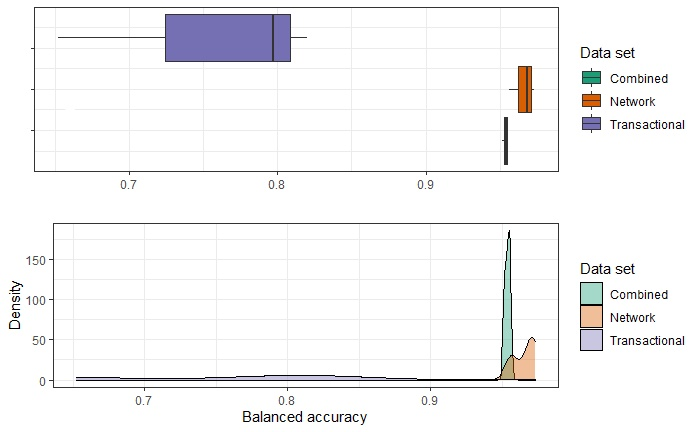
\includegraphics[scale = 0.6]{fig/CH3/data_sets_balance_acc_density_LI.jpg}
		\caption{A visual representation of the tested models balanced accuracy distribution grouped by the given input data set.}
		\label{fig:ch3_final_results_balanced_acc_density}
	\end{center}	
\end{figure}



% Ask Et: Should I include examples of the each input file (if needed)?
% Should I go into the details of how the simulator was run (instructions) virtual linux environment python files, bash files, etc?

%%%%%%%%%%%%%%%%%%%%%%%%%%%%%%%%%%%%%%%%%%%%%%%%
%
% start writing
%
%%%%%%%%%%%%%%%%%%%%%%%%%%%%%%%%%%%%%%%%%%%%%%%%

\chapter{Conclusion} \label{ch4_heading}

% reminded of projects premise
The project aimed to establish evidence suggesting
incorporating network metrics (derived using concepts of complex network analysis and graph theory) in the learning process (of a statistical model) can be advantageous for conventional anti-money laundering approaches. The rationale for the projects' hypothesis is that networks or graphs give us the ability to map \textit{relationships} in the real world \citep{baesens2015fraud}. Suppose the network analysis can capture these relationships components between entities. In that case, it can provide an additional dimension of information to the behaviour patterns on characteristics of money laundering banking clients. Therefore, possibly improving the identification and risk scoring sub-steps within the anti-money laundering process. The following chapter summarises the project's work, its findings, and makes suggestions for future work. 

\section{Project summary}
% chapter 2 - summary
To adequately address the projects research question, a comprehensive understanding of the three core elements of the project's methodology needed to be established. These elements are money laundering, machine learning, and network analytic's. The projects literature study, Chapter \ref{ch2_heading}, explained the elements mentioned above and investigated the research that has already been done. The chapter concluded by mentioning that there is evidence suggesting that network analytic's (extracting information from network or graphs) and machine learning (identifying complex non-linear patterns in data) can be used synergistically to produce stronger, more robust classification models. 

% chapter 3 - data generation and feature engneering
After conducting the literature study, a suitable framework or procedure for executing the project needed to be established. Figure \ref{fig:ch1_project_framework} gives an overview of the projects methodological procedure. This entire process is explained in detail in Chapter \ref{ch3_heading}. The first phase of the project was concerned with generating the project's raw data. The project used synthetically generated data using AMLSim, a multi-agent simulation platform specifically created to generate synthetic data for anti-money laundering research purposes \citep{AMLSim}. A detailed explanation of how the data simulator works can be found in section \ref{ch3_sub_heading_data}. Two financial data sets were generated using the data simulator - the raw training and testing data. The raw training data contained 12 043 accounts and 655 433 transactions, and the raw testing set contained 1446 accounts and 108 684 transactions. After generating the raw data, the project conducted an exploratory data analysis to establish an understanding of the data and validate the data simulators output. The project found that approximately 5\% of accounts were money laundering accounts, and  approximately 1\% of transactions were money laundering transactions in both data sets.
% chapter 3 - feature engineering
After the raw data was generated, the feature engineering process (Figure \ref{fig:ch1_project_framework}) could commence. The feature engineering process for the training and test raw data sets was identical. The feature engineering process took the raw data as input and produced three structured data tables. The first structures data table was the network feature data table. This data table was compiled by constructing an undirected weighted network and a directed network. The nodes in the networks would represent the bank accounts, and the network edges would represent the transactions between the accounts. After that, each network was decomposed into graph components of size $N>2$. Finally, the chosen network features or metrics could be extracted from each graph component. The complete network feature data table is illustrated in Table \ref{tab:ch3_network_features}. The second structured data table was the transactional feature data table. The project populated this table by creating useful transactional-based features from the raw data. Therefore, no network analysis was applied to construct the transactional feature data table. The complete transactional feature data table is illustrated in Table \ref{tab:ch3_trans_features}. The final structured data table was the combined feature data table. This table was constructed by combining the network feature data table with the transactional feature table. Therefore, joining the features shown in Table \ref{tab:ch3_network_features} and Table \ref{tab:ch3_trans_features}.\\
\\
The following sub-section described the modelling conducted in the project (sub-section \ref{ch3_sub_heading_modelling}). This section formed part of phase three of the project (Figure \ref{fig:ch1_project_framework}). The learning task of the project was a binary classification problem, where the model should predict, based on the set of input features given, if a bank account is involved in money laundering activity. The project defined two types of models. The first model was a logistic regression model and the second model was a neural network model. The modelling section provided a brief introduction to each model, explained the necessary data pre-processing that was conducted, and detailed the hyper-parameter tuning and training processes. The Chapter concluded with selecting the models it deemed fit to be tested on the testing data sets. The first model (``LR-ROC'') was a logistic regression model with L1 regularisation applied. The threshold value chosen for the model was based on the optimal threshold according to its ROC curve. The second model (``LR-PR'')  was identical to the first. However, the threshold value was chosen according to the optimal threshold value calculated from its precision-recall curve. The final model (``8-NN'') was the standard feed forward neural network model with 8 hidden neurons in its single hidden layer. A more detailed summary of each model and its chosen hyper-parameters is illustrated in Table \ref{tab:ch3_model_summary}.
% chapter 3 - Results
Chapter \ref{ch3_heading} concluded with the results obtained by each of the models when tested on each tests data set. The classification task of the project contained high-class imbalances in the response (mentioned as part of the EDA findings). Therefore, the performance metrics chosen needed to account for these severely skewed class distributions. The performance metrics chosen to evaluate each models performance on each of the data sets was the F1-score and balanced accuracy. The classification accuracy was also included, however, one should be cautious when jumping to conclusions using this metric (due to the accuracy paradox). Table \ref{tab:ch3_model_results} provides a summary of the test data set results for each model. On average, the network feature models (the models that used the network feature data set as their input) scored 0.371 higher on the F1-score than the transactional feature models. A similar result was obtained for the balanced accuracy, where the transactional feature models scored, on average, 0.21 less than the network feature models. Overall, the combined feature models performed slightly better or were equivalent to the network feature models. A visual representation of the results obtained is illustrated in Figure \ref{fig:ch3_final_results_bar}, Figure \ref{fig:ch3_final_results_f1_density}, and Figure \ref{fig:ch3_final_results_balanced_acc_density}.

\section{Findings and discussion}

% Comparing the trans models to the net models
The project's methodological process or framework was conducted so that the results will answer two essential questions. The first question is, \textit{how does the  performance of the statistical model, that used as input network features (derived from financial data) to predict money laundering accounts, compare to the same model but which uses transactional-based features as its input?} The project's results show that the network feature models significantly outperformed the transnational feature models. However, although the test results indicated the network feature models as the superior models, one should be critical about the results obtained. For example, how can one be sure that the project generated suitable transactional features? Or similarly, does there exist other transactional features that the project did not consider, which could have made a difference in the transactional model's performance? 

The second essential question is \textit{whether there is evidence that suggests that network features combined with transactional features deliver greater classification performance in predicting money laundering accounts?} From the test results, slight indications suggest combining the features sets could be beneficial. For example, models show marginally higher F1-score (Figure \ref{fig:ch3_final_results_f1_density}), and their balanced accuracy distributions are much narrower than the  network feature models (Figure \ref{fig:ch3_final_results_balanced_acc_density}). However, looking at the results holistically suggests that there is not much improvement in combining the feature sets. Again looking at the results from a critical point of view, there are some things the project could have implemented to possibly change this result. For example, suppose some formal feature selection (best-subset, forward/backward selection, etc.) or feature extraction (principal component analysis or Isometric mapping) was introduced. In that case, it could have selected only the more valuable'' features, reducing the noise within the data, and making the learning task easier. A final remark to consider is that even though the performance increase of the combined feature models was marginal to that of the network feature models, in reality, this would still be an improvement to an anti-money laundering process. This incremental improvement can significantly reduce the colossal loss commercial banks experience through money laundering activity.   

\section{Future work}

Throughout the project, particular research ``opportunities'' presented themselves. Conducting further research on any of these topics will be intriguing to see how they change the outcomes provided in the project. The main idea of each research opportunity is as follows:

\begin{itemize}
    \item \textit{Time-weighted network}: \citet{van2017gotcha} defined a time-weighted network where the weight assigned to each edge in the graph decays based on some decaying constant, $\gamma$. The assumption was made that nodes with more frequent contact with each other exhibit stronger relationships. The idea of incorporating a decaying constant into the project undirected weighted graph might provide a more realistic view of the accounts current relationship with each other. 
    
    \item \textit{Increasing project's scale}: The project was conducted on a relatively small scale i.t.o the number of accounts and transactions used. In a commercial bank, there can be anything from 1M to 10M banking clients and up to 1B transactions (depending on the historical time frame chosen). Therefore, it would be interesting to see how the project's implementation framework scales to such sizes and how the results are affected.
    
    \item \textit{Investigating specific money typologies:} The project took a very broad approach in analysing all the money laundering typologies the AMLSim has to offer. However, it would be valuable to establish what network features (or combined with transactional features) help predict different types of money laundering typologies.
    
    \item \textit{Apply the project's framework to actual financial data:} The project used synthetically generated financial data. Although the simulator used to generate the data is very intricate, it would still be interesting to see if similar results are obtained by using actual financial data of a commercial bank.    
    
\end{itemize}






%=================================================
% bibliography
%=================================================
%\cite{*} % cites all items in your .bib file for the purpose of testing biblatex - REMOVE!
\printbibliography[heading=bibintoc] % prints a bibliography containing all (and only) cited items


%=================================================
% Appendices
%=================================================
\appendix
\chapter{Tables} \label{app_1}

% 1. CH3 - Table of variables excluded from raw data tables
\begin{sidewaystable}[ht]
\begin{adjustbox}{center}
\begin{tabular}{cll}
\hline
\multicolumn{1}{l}{\textbf{Raw data table}} & \textbf{Feature name} & \textbf{Reason for exclusion from analysis}                                                                                                                                                                      \\ \hline
\multirow{9}{*}{\texttt{accounts.csv}}               & \texttt{dsply\_nm}             & Identical to \texttt{acct\_id} feature.                                                                                                                                                                                   \\
                                            & \texttt{ty}pe                  & Singular value feature.                                                                                                                                                                                          \\
                                            & \texttt{acct\_stat}            & Singular value feature.                                                                                                                                                                                          \\
                                            & \texttt{acct\_rptng\_crncy}    & Singular value feature.                                                                                                                                                                                          \\
                                            & \texttt{branch\_id}            & Singular value feature.                                                                                                                                                                                          \\
                                            & \texttt{open\_dt}              & Singular value feature.                                                                                                                                                                                          \\
                                            & \texttt{close\_dt}             & Singular value feature.                                                                                                                                                                                          \\
                                            & \texttt{tx\_bahavior\_id}      & \begin{tabular}[c]{@{}l@{}}It indicates which accounts are \\ fraudulent and which are not. \\ Similar to the response used \\ (\texttt{prior\_sar\_count}), therefore excluded.\end{tabular}                             \\
                                            & \texttt{bank\_id}              & Singular value feature.                                                                                                                                                                                          \\ \hline
\multirow{2}{*}{\texttt{alert\_transactions.csv}}    & \texttt{tx\_type}              & Singular value feature.                                                                                                                                                                                          \\
                                            & \texttt{is\_sar}               & \begin{tabular}[c]{@{}l@{}}Singular value feature. If a transaction was \\ in the \texttt{alert\_transaction.csv} then \\ it was automatically classified as being a \\ money-laundering transaction\end{tabular}            \\ \hline
\multirow{5}{*}{\texttt{alert\_accounts.csv}}        & \texttt{is\_sar}              & \begin{tabular}[c]{@{}l@{}}Singular value feature. If an account was in \\ the \texttt{alert\_accounts.csv}, then the account \\ was automatically classified as taking part \\ in money-laundering activities.\end{tabular} \\
                                            & \texttt{schedule\_id}          & Singular value feature.                                                                                                                                                                                          \\
                                            & \texttt{bank\_id}              & Singular value feature.                                                                                                                                                                                          \\
                                            & \texttt{start}                 & Singular value feature.                                                                                                                                                                                          \\
                                            & \texttt{end}                   & Singular value feature.                                                                                                                                                                                         
\end{tabular}
\end{adjustbox}
\caption{The table summarises all the raw data features excluded from the analysis. In addition, the table provides the name of the raw data table, the features excluded from the raw data table, and the reason thereof.}
\label{tab:ch3_raw_features_removed}
\end{sidewaystable}

% 2. CH3 - Network features 
\begin{sidewaystable}[ht]
\begin{adjustbox}{scale=0.6,center}
\begin{tabular}{lll|lll}
\hline
\textbf{\begin{tabular}[c]{@{}l@{}}Feature \\ number\end{tabular}} & \textbf{Feature name}                   & \textbf{Description}                                                                                                                                                                   & \textbf{\begin{tabular}[c]{@{}l@{}}Feature \\ number\end{tabular}} & \textbf{Feature name}     & \textbf{Description}                                                                                                                                                                                                             \\ \hline
1                                                                  & \texttt{acct\_id}                                & Unique ID for bank account.                                                                                                                                                            & 16                                                                 & \texttt{closeness\_centrality}     & \begin{tabular}[c]{@{}l@{}}The average distance from an account to all \\ other accounts (measured by the number of ``hops'').\end{tabular}                                                                                      \\ \hline
2                                                                  & \texttt{transitivity}                            & \begin{tabular}[c]{@{}l@{}}The cluster coefficient for an account \\ (see calculation in Table X).\end{tabular}                                                                        & 17                                                                 & \texttt{farness}                   & Is the reciprocal of the closeness centrality.                                                                                                                                                                                   \\ \hline
3                                                                  & \texttt{total\_degree}                           & \begin{tabular}[c]{@{}l@{}}The total number of  ``connections'' an account has.\\ This corresponds to the total amount of edges of a node.\end{tabular}                                & 18                                                                 & \texttt{eigen\_vector\_centrality} & \begin{tabular}[c]{@{}l@{}}The eigenvector centrality score corresponds to the \\ values of the first eigenvector of the graph adjacency \\ matrix (see calculation in Table X).\end{tabular}                                    \\ \hline
4                                                                  & \texttt{fraud\_degree}                           & \begin{tabular}[c]{@{}l@{}}The number of money laundering accounts \\ connected to an account.\end{tabular}                                                                            & 19                                                                 & \texttt{betweenness}               & \begin{tabular}[c]{@{}l@{}}Counts the number of times an account lies on the geodesic \\ between any accounts nodes in the network.\end{tabular}                                                                                 \\ \hline
5                                                                  & \texttt{non\_fraud\_degree}                      & \begin{tabular}[c]{@{}l@{}}The number of honest accounts \\ connected to an account.\end{tabular}                                                                                      & 20                                                                 & \texttt{avg\_geodesic}             & \begin{tabular}[c]{@{}l@{}}The average geodesic is the average of the shortest paths \\ between an account and all the other accounts.\end{tabular}                                                                              \\ \hline
6                                                                  & \texttt{degree\_strenght}                        & \begin{tabular}[c]{@{}l@{}}The total transactional amount received and payed \\ by an account.\end{tabular}                                                                            & 21                                                                 & \texttt{page\_rank\_base}          & An accounts PageRank value (see calculation in Table X).                                                                                                                                                                         \\ \hline
7                                                                  & \texttt{node\_density}                           & \begin{tabular}[c]{@{}l@{}}The ratio of the number of connections and \\ a number of possible connections an account can have.\end{tabular}                                            & 22                                                                 & \texttt{page\_rank\_fraud}         & \begin{tabular}[c]{@{}l@{}}An accounts PageRank value if the starting vector \\ (usually a vector of ones) is defined as a zero value \\ for honest accounts and a non-zero value for money \\ laundering accounts.\end{tabular} \\ \hline
8                                                                  & \texttt{relational\_neighbour\_not\_fraud}       & \begin{tabular}[c]{@{}l@{}}The ratio of a accounts' neighbours that are not participating \\ money laundering activity.\end{tabular}                                                   & 23                                                                 & \texttt{in\_degree}                & \begin{tabular}[c]{@{}l@{}}The frequency of an account total number of incoming\\ transactions (payments received).\end{tabular}                                                                                                 \\ \hline
9                                                                  & \texttt{relational\_neighbour\_fraud}            & \begin{tabular}[c]{@{}l@{}}The ratio of a accounts' neighbours that are \\ participating money laundering activity.\end{tabular}                                                       & 24                                                                 & \texttt{in\_degree\_fraud}         & \begin{tabular}[c]{@{}l@{}}The frequency of the total number of money laundering \\ transactions an account has received.\end{tabular}                                                                                           \\ \hline
10                                                                 & \texttt{prob\_relational\_neighbour\_not\_fraud} & \begin{tabular}[c]{@{}l@{}}The relative number of neighbours of an account which \\ are honest.\end{tabular}                                                                           & 25                                                                 & \texttt{in\_degree\_non\_fraud}    & \begin{tabular}[c]{@{}l@{}}The frequency of the total number of honest \\ transactions an account has received.\end{tabular}                                                                                                     \\ \hline
11                                                                 & \texttt{prob\_relational\_neighbour\_fraud}      & \begin{tabular}[c]{@{}l@{}}The relative number of neighbours of an account which \\ are involved in money laundering activity.\end{tabular}                                            & 26                                                                 & \texttt{out\_degree}               & \begin{tabular}[c]{@{}l@{}}The frequency of an account total number of outgoing\\ transactions (payments made).\end{tabular}                                                                                                     \\ \hline
12                                                                 & \texttt{total\_triangles}                        & \begin{tabular}[c]{@{}l@{}}The total number of fully connected subgraphs (consisting of three accounts) \\ an account is a part of.\end{tabular}                                       & 27                                                                 & \texttt{out\_degree\_fraud}        & \begin{tabular}[c]{@{}l@{}}The frequency of the total number of money laundering \\ transactions an account has made.\end{tabular}                                                                                               \\ \hline
13                                                                 & \texttt{legit\_triangles}                        & \begin{tabular}[c]{@{}l@{}}The total number of triangles an account is part of that only consists of \\ other honest accounts.\end{tabular}                                            & 28                                                                 & \texttt{out\_degree\_non\_fraud}   & \begin{tabular}[c]{@{}l@{}}The frequency of the total number of honest \\ transactions an account has made.\end{tabular}                                                                                                         \\ \hline
14                                                                 & \texttt{semi\_fraud\_triangles}                  & \begin{tabular}[c]{@{}l@{}}The total number of triangles an account is part of that consists of \\ other honest accounts and accounts involved money laundering activity.\end{tabular} & 29                                                                 & \texttt{is\_fraud}                 & \begin{tabular}[c]{@{}l@{}}The response variable, indicating if an \\ an account is a money-laundering account.\end{tabular}                                                                                                     \\ \hline
15                                                                 & \texttt{fraud\_triangles}                        & \begin{tabular}[c]{@{}l@{}}The total number of triangles an account is part of that only consists of \\ other accounts involved in money laundering activity.\end{tabular}             &                                                                    &                           &                                                                                                                                                                                                                                  \\ \hline
\end{tabular}
\end{adjustbox}
\caption{The finalised network features and a short description of each. Features 1-22 was constructed from the undirected weighted graph components, and features 23-28 was constructed from the directed graph components.}
\label{tab:ch3_network_features}
\end{sidewaystable}

% 3. CH3 - Transactional features 
\begin{sidewaystable}[ht]
\begin{adjustbox}{scale=0.7}
\begin{tabular}{lll|lll}
\hline
\textbf{\begin{tabular}[c]{@{}l@{}}Feature \\ number\end{tabular}} & \textbf{\begin{tabular}[c]{@{}l@{}}Feature \\ name\end{tabular}} & \textbf{\begin{tabular}[c]{@{}l@{}}Feature \\ description\end{tabular}}                                                                                                       & \textbf{\begin{tabular}[c]{@{}l@{}}Feature \\ number\end{tabular}} & \textbf{\begin{tabular}[c]{@{}l@{}}Feature \\ name\end{tabular}} & \textbf{\begin{tabular}[c]{@{}l@{}}Feature \\ description\end{tabular}}                                                                                          \\ \hline
1                                                                  & \texttt{acct\_id}                                                         & Unique ID for bank account.                                                                                                                                                   & 13                                                                 & \texttt{outgoing\_min}                                                    & The minimum payment amount an account makes.                                                                                                                     \\ \hline
2                                                                  & \texttt{init\_balance}                                                    & \begin{tabular}[c]{@{}l@{}}Initial balance when the client created \\ the account.\end{tabular}                                                                               & 14                                                                 & \texttt{outgoing\_round\_numbers\_count}                                  & \begin{tabular}[c]{@{}l@{}}The frequency of transactions made by \\ an account that is a rounded amount, \\ for example (R1000 as opposed to R999).\end{tabular} \\ \hline
3                                                                  & \texttt{incoming\_total}                                                  & \begin{tabular}[c]{@{}l@{}}The total transactional amount of payments \\ received by the account.\end{tabular}                                                                & 15                                                                 & \texttt{total\_non\_fraud\_payments}                                      & \begin{tabular}[c]{@{}l@{}}The total transactional amount of payments \\ made by the account to honest accounts.\end{tabular}                                    \\ \hline
4                                                                  & \texttt{incoming\_avg}                                                   & \begin{tabular}[c]{@{}l@{}}The average incoming transactional amount \\ an account receives.\end{tabular}                                                                     & 16                                                                 & \texttt{total\_fraud\_payments}                                           & \begin{tabular}[c]{@{}l@{}}The total transactional amount of payments \\ made by the account that is to money \\ laundering accounts.\end{tabular}               \\ \hline
5                                                                  & \texttt{incoming\_max}                                                    & \begin{tabular}[c]{@{}l@{}}The maximum incoming transactional amount \\ an account receives.\end{tabular}                                                                     & 17                                                                 & \texttt{receive\_period\_max}                                            & \begin{tabular}[c]{@{}l@{}}The maximum time that has passed since \\ the account has received a payment.\end{tabular}                                            \\ \hline
6                                                                  & \texttt{incoming\_min}                                                    & \begin{tabular}[c]{@{}l@{}}The minimum incoming transactional amount \\ an account receives.\end{tabular}                                                                     & 18                                                                 & \texttt{receive\_period\_min}                                             & \begin{tabular}[c]{@{}l@{}}The minimum time that has passed since \\ the account has received a payment.\end{tabular}                                            \\ \hline
7                                                                  & \texttt{incoming\_round\_numbers\_count}                                  & \begin{tabular}[c]{@{}l@{}}The frequency of incoming transactions received by \\ an account that is a rounded amount, \\ for example (R1000 as opposed to R999).\end{tabular} & 19                                                                 & \texttt{receive\_period\_avg}                                             & \begin{tabular}[c]{@{}l@{}}The average time that has passed since \\ the account has received a payment.\end{tabular}                                            \\ \hline
8                                                                  & \texttt{non\_fraud\_total\_income}                                        & \begin{tabular}[c]{@{}l@{}}The total transactional amount of payments \\ received by the account that is from honest accounts.\end{tabular}                                   & 20                                                                 & \texttt{payment\_period\_max}                                            & \begin{tabular}[c]{@{}l@{}}The maximum time that has passed since \\ the account has made a payment.\end{tabular}                                                \\ \hline
9                                                                  & \texttt{fraud\_total\_income}                                            & \begin{tabular}[c]{@{}l@{}}The total transactional amount of payments \\ received by the account that is from money \\ laundering accounts.\end{tabular}                      & 21                                                                 & \texttt{payment\_period\_min}                                             & \begin{tabular}[c]{@{}l@{}}The minimum time that has passed since \\ the account has made a payment.\end{tabular}                                                \\ \hline
10                                                                 & \texttt{outgoing\_total}                                                  & \begin{tabular}[c]{@{}l@{}}The total transactional amount of payments \\ made by the account.\end{tabular}                                                                    & 22                                                                 & \texttt{payment\_period\_avg}                                             & \begin{tabular}[c]{@{}l@{}}The average time that has passed since \\ the account has made a payment.\end{tabular}                                                \\ \hline
11                                                                 & \texttt{outgoing\_avg}                                                    & \begin{tabular}[c]{@{}l@{}}The average outgoing transactional \\ amount of an account.\end{tabular}                                                                           & 23                                                                 & \texttt{is\_fraud}                                                       & \begin{tabular}[c]{@{}l@{}}The response variable, indicating if an \\ an account is a money-laundering account.\end{tabular}                                     \\ \hline
12                                                                 & \texttt{outgoing\_max}                                                    & The maximum payment amount an account makes.                                                                                                                                  &                                                                    &                                                                  &                                                                                                                                                                  \\ \hline
\end{tabular}
\end{adjustbox}
\caption{A table of the transactional features and a short description of each used for the finalised transactional feature data set.}
\label{tab:ch3_trans_features}
\end{sidewaystable}

% 4. Confusion matrices %%%

% LR-ROC - Network
\begin{table}
\centering
\begin{tabular}{llll}
                                                        &   & \multicolumn{2}{c}{\textbf{Actual}} \\
                                                        &   & False             & True            \\ \hline
\multicolumn{1}{c}{\multirow{2}{*}{\textbf{Predicted}}} & 0 & 1182              & 3               \\
\multicolumn{1}{c}{}                                    & 1 & 56                & 69              \\ \hline
\end{tabular}
\caption{Confusion matrix of the LR-ROC model applied to the test network feature data set.}
\label{tab:ch3_cm_LR_ROC_network}
\end{table}

% LR-PR - Network
\begin{table}
\centering
\begin{tabular}{llll}
                                                        &   & \multicolumn{2}{c}{\textbf{Actual}} \\
                                                        &   & False             & True            \\ \hline
\multicolumn{1}{c}{\multirow{2}{*}{\textbf{Predicted}}} & 0 & 1212              & 3               \\
\multicolumn{1}{c}{}                                    & 1 & 26                & 69              \\ \hline
\end{tabular}
\caption{Confusion matrix of the LR-PR model applied to the test network feature data set.}
\label{tab:ch3_cm_LR_PR_network}
\end{table}

% (8)-Network - Network
\begin{table}
\centering
\begin{tabular}{llll}
                                                        &   & \multicolumn{2}{c}{\textbf{Actual}} \\
                                                        &   & False             & True            \\ \hline
\multicolumn{1}{c}{\multirow{2}{*}{\textbf{Predicted}}} & 0 & 1223              & 3               \\
\multicolumn{1}{c}{}                                    & 1 & 15                & 69              \\ \hline
\end{tabular}
\caption{Confusion matrix of the (8)-NN model applied to the test network feature data set.}
\label{tab:ch3_cm_nn_network}
\end{table}

% LR-ROC - Trans
\begin{table}
\centering
\begin{tabular}{llll}
                                                        &   & \multicolumn{2}{c}{\textbf{Actual}} \\
                                                        &   & False             & True            \\ \hline
\multicolumn{1}{c}{\multirow{2}{*}{\textbf{Predicted}}} & 0 & 1051              & 15              \\
\multicolumn{1}{c}{}                                    & 1 & 187               & 57              \\ \hline
\end{tabular}
\caption{Confusion matrix of the LR-ROC model applied to the test transactional feature data set.}
\label{tab:ch3_cm_LR_ROC_trans}
\end{table}

% LR-PR - Trans
\begin{table}
\centering
\begin{tabular}{llll}
                                                        &   & \multicolumn{2}{c}{\textbf{Actual}} \\
                                                        &   & False             & True            \\ \hline
\multicolumn{1}{c}{\multirow{2}{*}{\textbf{Predicted}}} & 0 & 1199              & 27              \\
\multicolumn{1}{c}{}                                    & 1 & 39                & 45              \\ \hline
\end{tabular}
\caption{Confusion matrix of the LR-PR model applied to the test transactional feature data set.}
\label{tab:ch3_cm_LR_PR_trans}
\end{table}

% 8-NN - Trans
\begin{table}
\centering
\begin{tabular}{llll}
                                                        &   & \multicolumn{2}{c}{\textbf{Actual}} \\
                                                        &   & False             & True            \\ \hline
\multicolumn{1}{c}{\multirow{2}{*}{\textbf{Predicted}}} & 0 & 1201              & 48              \\
\multicolumn{1}{c}{}                                    & 1 & 37                & 24              \\ \hline
\end{tabular}
\caption{Confusion matrix of the (8)-NN model applied to the test transactional feature data set.}
\label{tab:ch3_cm_nn_trans}
\end{table}

% LR-ROC - Combined
\begin{table}
\centering
\begin{tabular}{llll}
                                                        &   & \multicolumn{2}{c}{\textbf{Actual}} \\
                                                        &   & False             & True            \\ \hline
\multicolumn{1}{c}{\multirow{2}{*}{\textbf{Predicted}}} & 0 & 1180              & 3               \\
\multicolumn{1}{c}{}                                    & 1 & 58                & 69              \\ \hline
\end{tabular}
\caption{Confusion matrix of the LR-ROC model applied to the test combined feature data set.}
\label{tab:ch3_LR_ROC_all}
\end{table}

% LR-PR - Combined
\begin{table}
\centering
\begin{tabular}{llll}
                                                        &   & \multicolumn{2}{c}{\textbf{Actual}} \\
                                                        &   & False             & True            \\ \hline
\multicolumn{1}{c}{\multirow{2}{*}{\textbf{Predicted}}} & 0 & 1222              & 6               \\
\multicolumn{1}{c}{}                                    & 1 & 16                & 66              \\ \hline
\end{tabular}
\caption{Confusion matrix of the LR-PR model applied to the test combined feature data set.}
\label{tab:ch3_LR_PR_all}
\end{table}

% NN-8 - Combined
\begin{table}[t!]
\centering
\begin{tabular}{llll}
                                                        &   & \multicolumn{2}{c}{\textbf{Actual}} \\
                                                        &   & False             & True            \\ \hline
\multicolumn{1}{c}{\multirow{2}{*}{\textbf{Predicted}}} & 0 & 1228              & 6               \\
\multicolumn{1}{c}{}                                    & 1 & 10                & 66              \\ \hline
\end{tabular}
\caption{Confusion matrix of the (8)-NN model applied to the test combined feature data set.}
\label{tab:ch3_nn_all}
\end{table}


\chapter{Figures} \label{app_2}

% 1. raw data EDA figures
\begin{figure}[]
	\begin{center}
		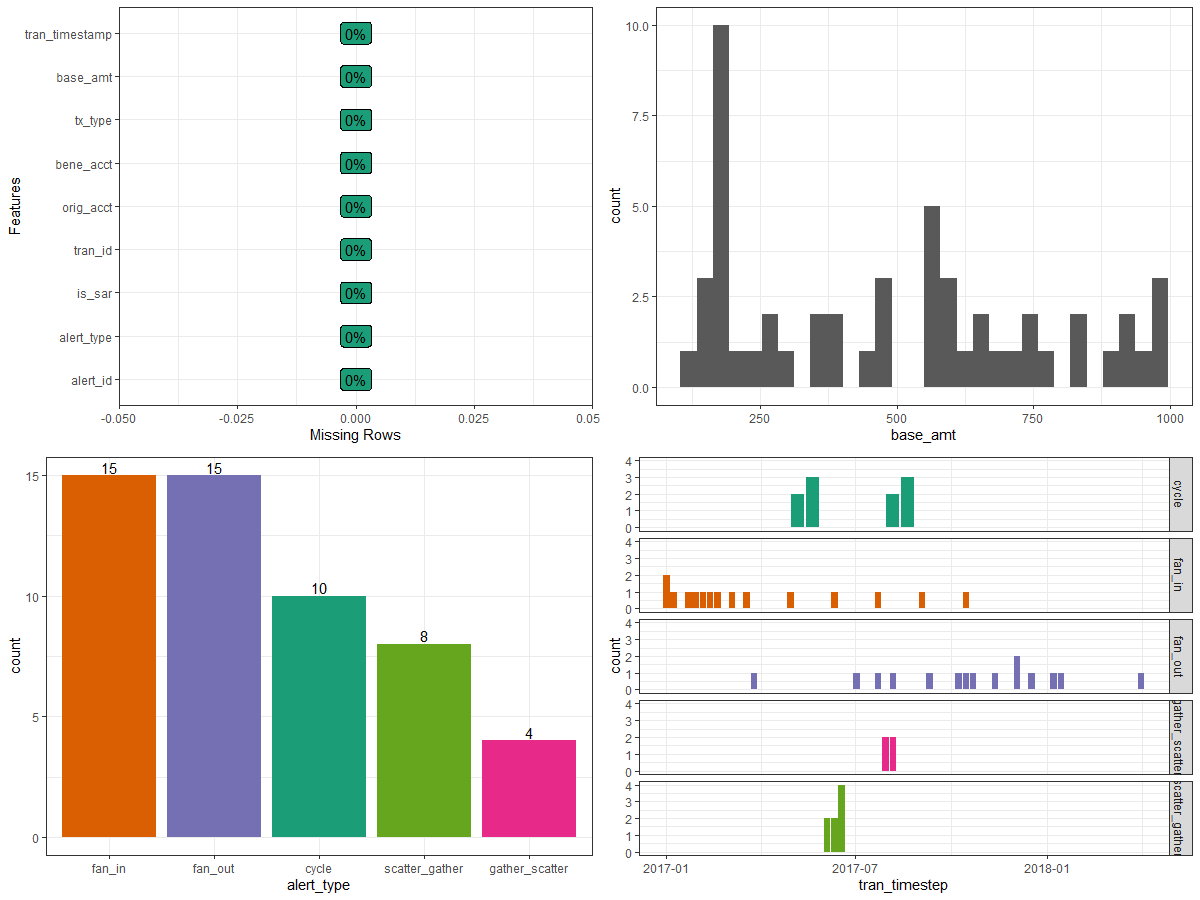
\includegraphics[scale=0.5]{fig/CH3/test_alrt_trans_summary.png}
		\caption{Example of the visualisations generated during the EDA of the test \texttt{alert\_transactions.csv} file. (top-left) The missing values profile. (top-right) Histogram of the transaction amount (\texttt{base\_amount}). (bottom-left) Frequency bar chart of the occurrences of different money laundering typologies (\texttt{alert\_type}) among the account transactions. (bottom-right) A timeline plot of when the different money laundering typologies occurred.}
		\label{fig:ch3_raw_eda_test_alrt_trans_sum}
	\end{center}	
\end{figure}

\begin{figure}[]
	\begin{center}
		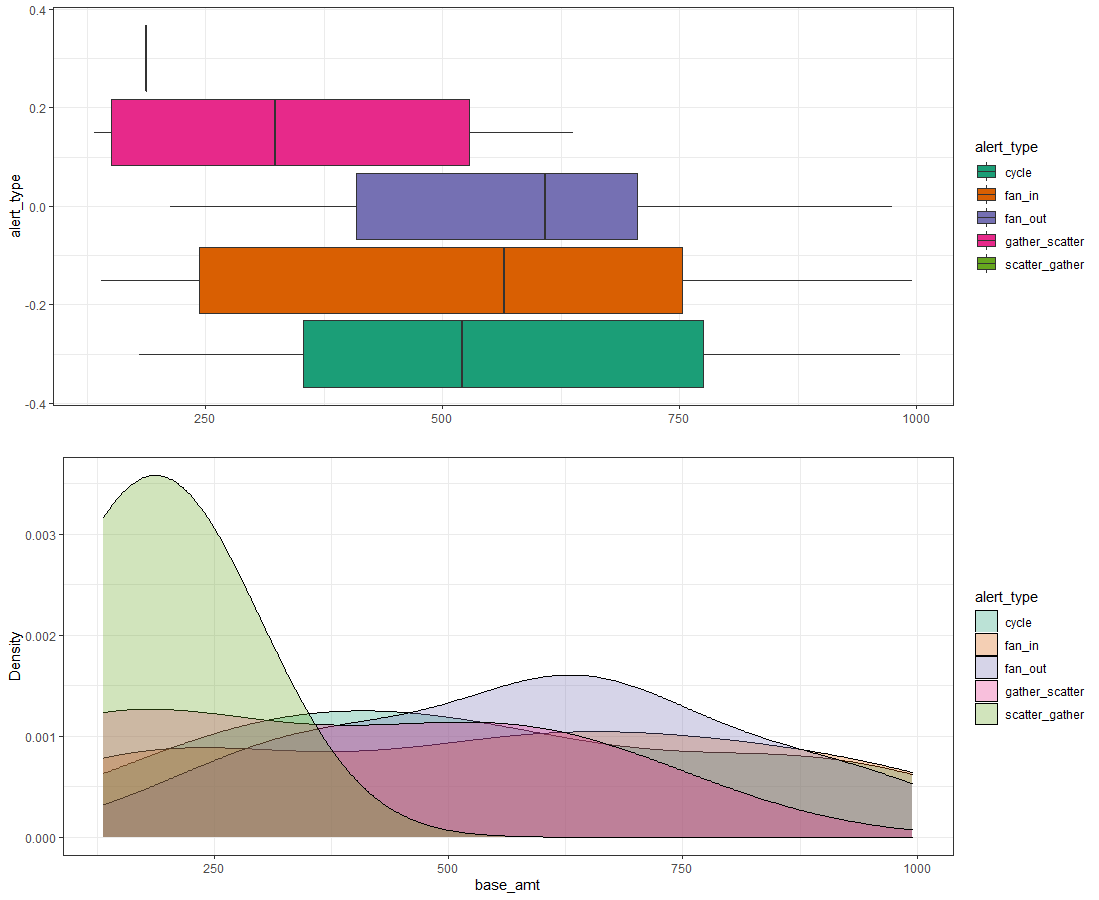
\includegraphics[scale=0.5]{fig/CH3/test_alrt_trans_tx_amount_alert_type_distribution.jpg}
		\caption{Both plots show the transaction amount distribution (top - box and whiskers and bottom - density plot) of transactions that were classified as being money laundering transactions for the test \texttt{alert\_transactions.csv} file.}
		\label{fig:ch3_raw_eda_test_alrt_trans_tx_distr}
	\end{center}	
\end{figure}

\begin{figure}[]
	\begin{center}
		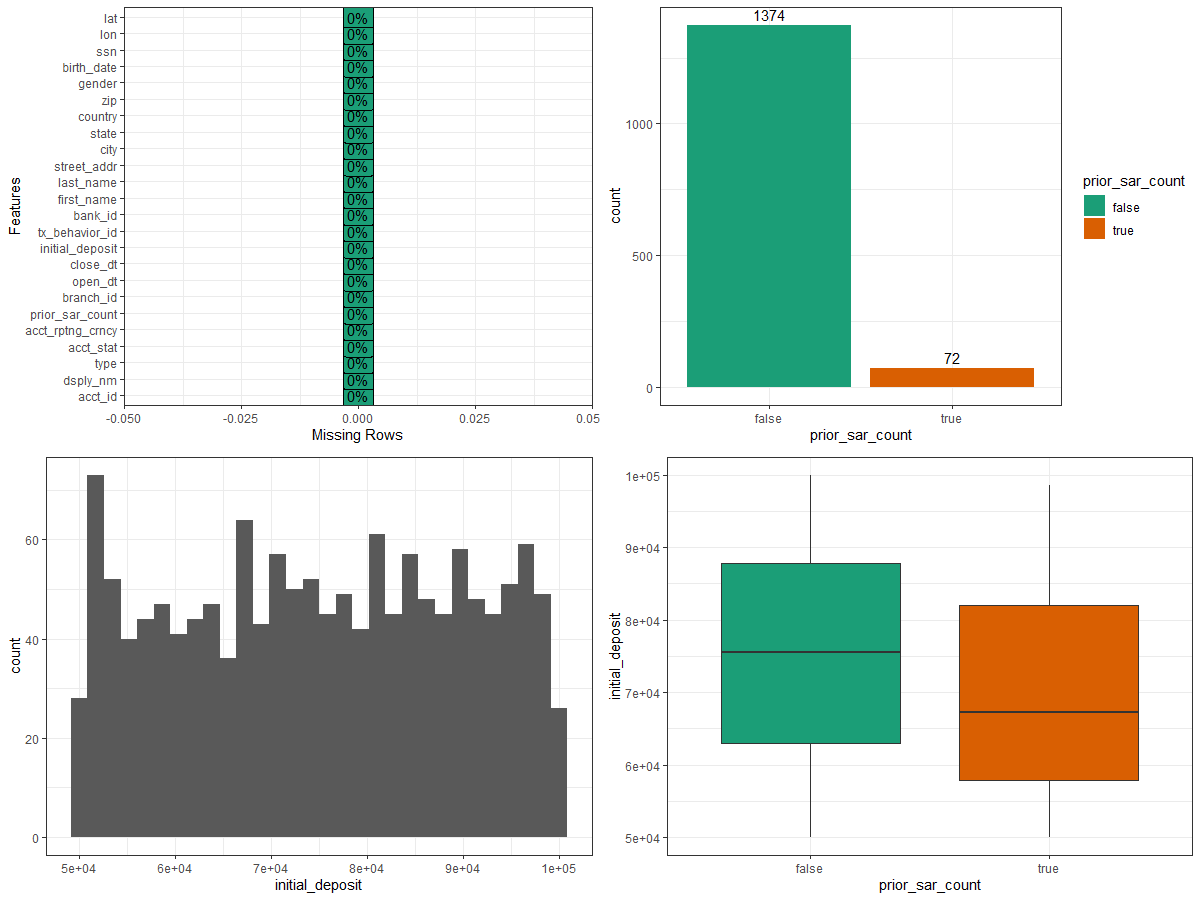
\includegraphics[scale=0.5]{fig/CH3/test_acc_summary.png}
		\caption{Example of the visualisations generated during the EDA of the test \texttt{accounts.csv} file. (top-left) The missing values profile. (top-right) Frequency bar chart of accounts that did and did not participate in money laundering activity. (bottom-left) Histogram of the accounts initial balances (\texttt{initial\_deposit}. (bottom-right) A box and whiskers plot showing money laundering and honest account's initial deposits.}
		\label{fig:ch3_raw_eda_test_acct_sum}
	\end{center}	
\end{figure}

% 2. 10-fold cross-validation lambda figures (transactional and combined)  
\begin{figure}[]
	\begin{center}
		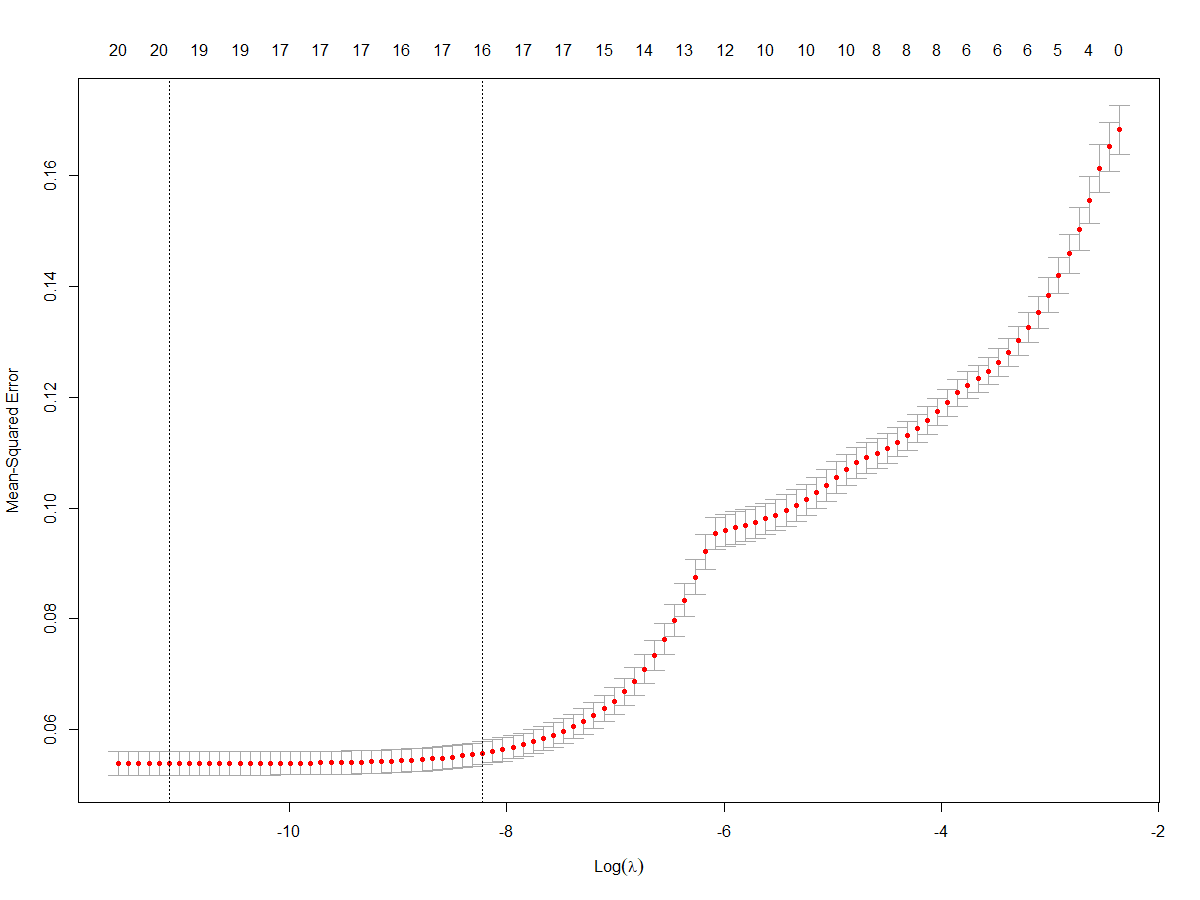
\includegraphics[scale=0.45]{fig/CH3/cv_lambda_trans.png}
		\caption{Ten-fold cross-validation mean square error (MSE) for the L1 regularised logistic regression model applied to the transactional feature data set. The vertical dashed line on the left is the $log(\lambda)$ value of where the MSE is at its minimum and the vertical on the right is the largest $log(\lambda)$ value such that the MSE is within one standard error of the minimum MSE. Also, the plot illustrates at the top, the number of positive weights $\boldsymbol{w} > 0$ at a specific $log(\lambda)$ value.}
		\label{fig:ch3_lr_lambda_cv_trans}
	\end{center}	
\end{figure}

\begin{figure}[]
	\begin{center}
		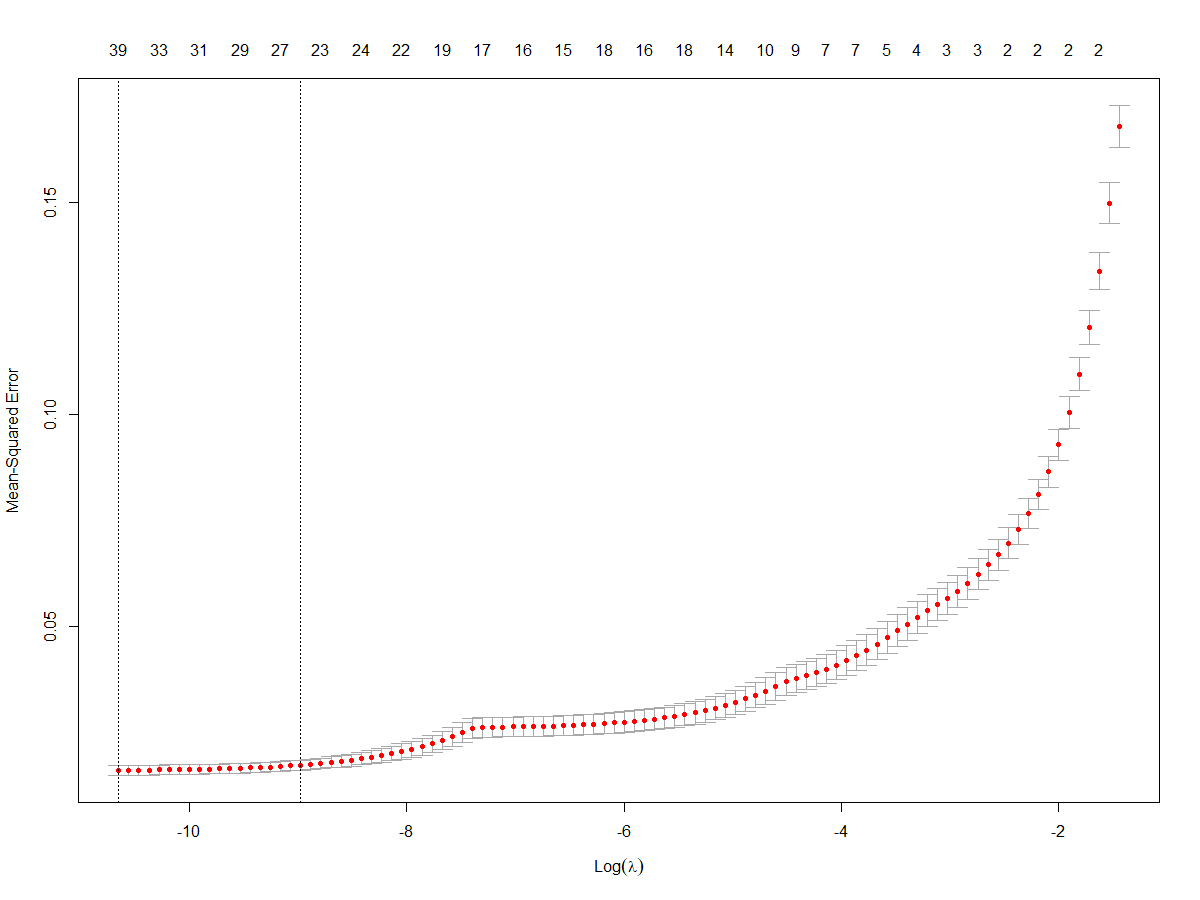
\includegraphics[scale=0.45]{fig/CH3/cv_lambda_all.png}
		\caption{Ten-fold cross-validation mean square error (MSE) for the L1 regularised logistic regression model applied to the combined feature data set. The vertical dashed line on the left is the $log(\lambda)$ value of where the MSE is at its minimum and the vertical on the right is the largest $log(\lambda)$ value such that the MSE is within one standard error of the minimum MSE. Also, the plot illustrates at the top, the number of positive weights $\boldsymbol{w} > 0$ at a specific $log(\lambda)$ value.}
		\label{fig:ch3_lr_lambda_cv_all}
	\end{center}	
\end{figure}

% validation curves NN -  (8)- transactional
\begin{figure}[]
	\begin{center}
		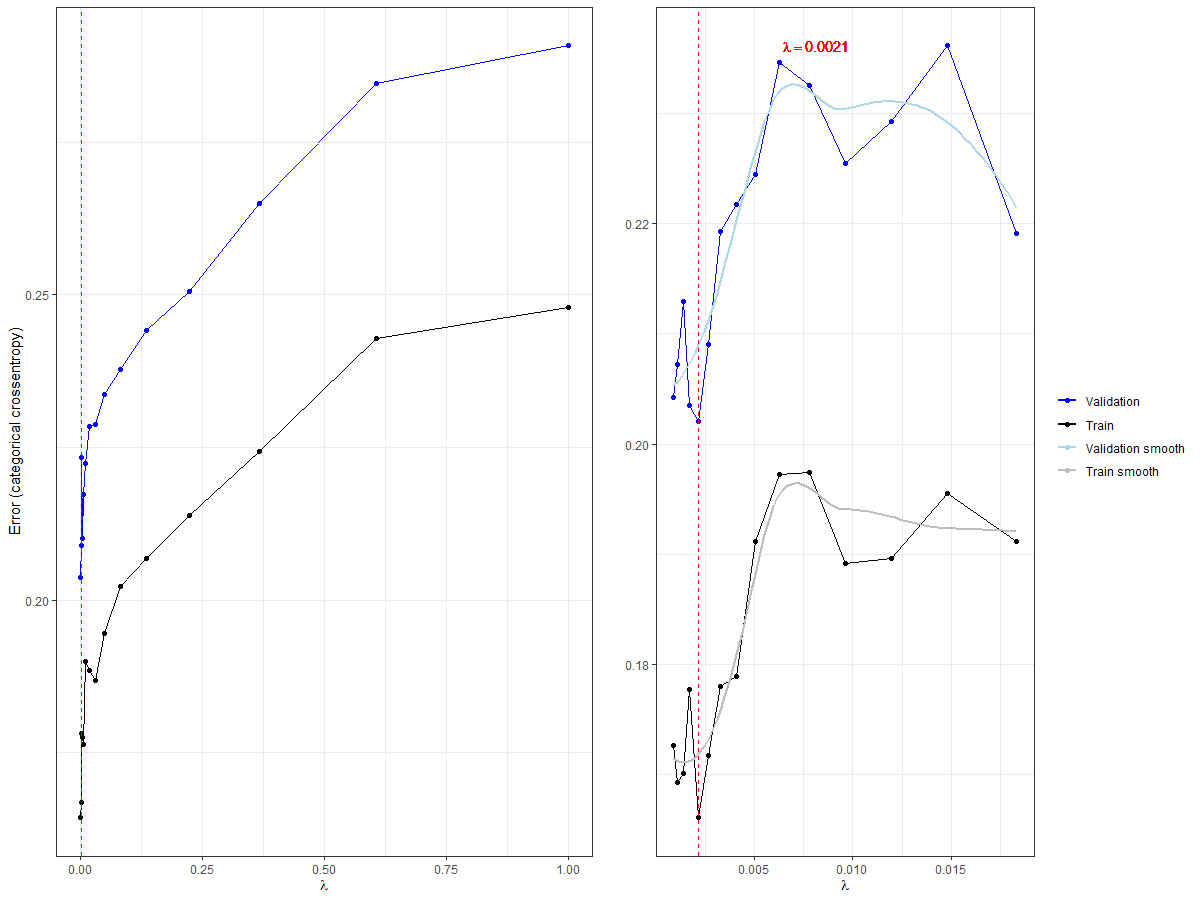
\includegraphics[scale = 0.5]{fig/CH3/trans_mod_1_lambda_plot.png}
		\caption{The plot illustrates the process of selecting the best approximate $\lambda$ value for the (8)-network model applied to the transactional feature data set. (left) The training and validation set errors for a range of $\lambda$ values. (right) The training and validation set errors for a more specific range of $\lambda$ values. The training and validation error smooth curves are additional curves to help view the curve patterns. Also, the $\lambda$ value that produced the minimum validation error is shown in both plots.}
		\label{fig:ch3_nn_validation_mod1_trans}
	\end{center}	
\end{figure}

% validation curves NN -  (64)- transactional
\begin{figure}[]
	\begin{center}
		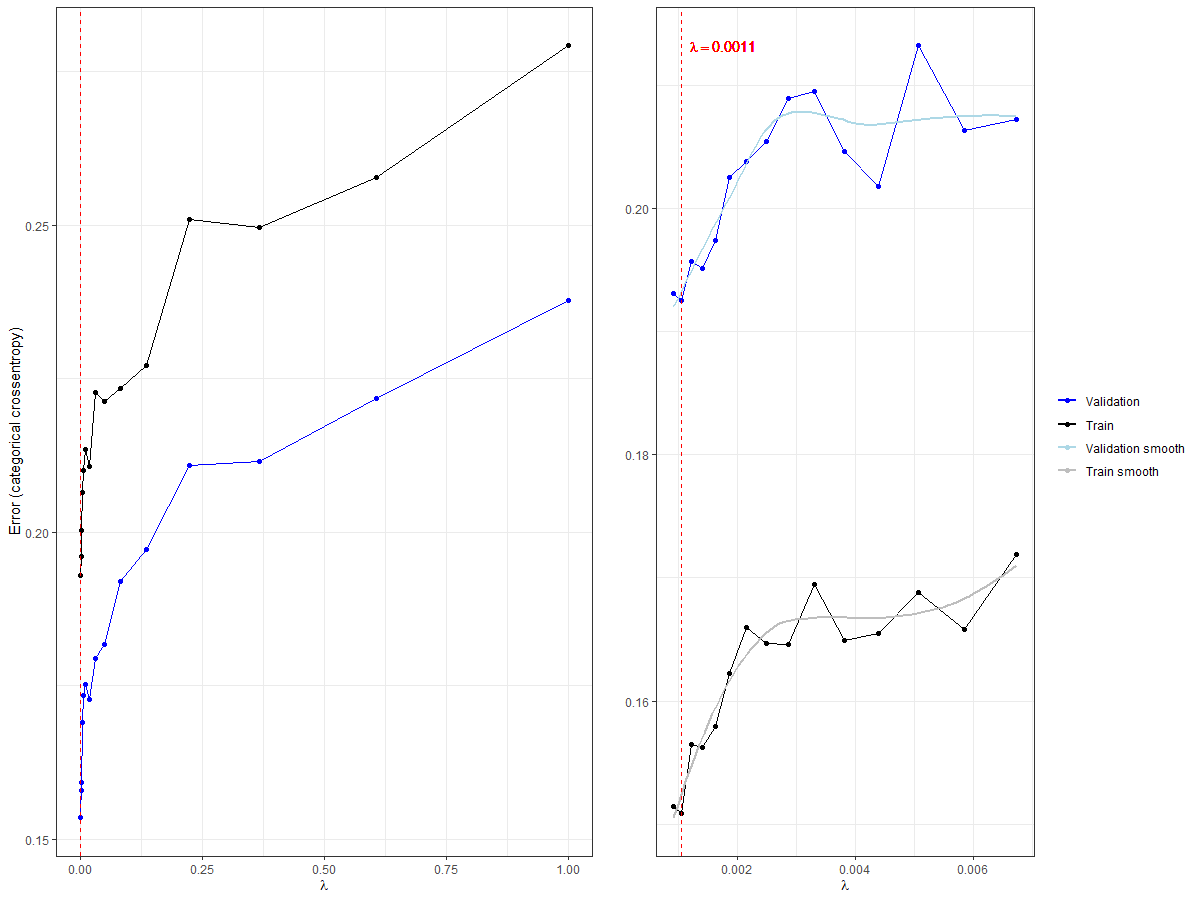
\includegraphics[scale = 0.5]{fig/CH3/trans_mod_2_lambda_plot.png}
		\caption{The plot illustrates the process of selecting the best approximate $\lambda$ value for the (64)-network model applied to the transactional feature data set. (left) The training and validation set errors for a range of $\lambda$ values. (right) The training and validation set errors for a more specific range of $\lambda$ values. The training and validation error smooth curves are additional curves to help view the curve patterns. Also, the $\lambda$ value that produced the minimum validation error is shown in both plots.}
		\label{fig:ch3_nn_validation_mod2_trans}
	\end{center}	
\end{figure}

% validation curves NN -  (8)- combines
\begin{figure}[]
	\begin{center}
		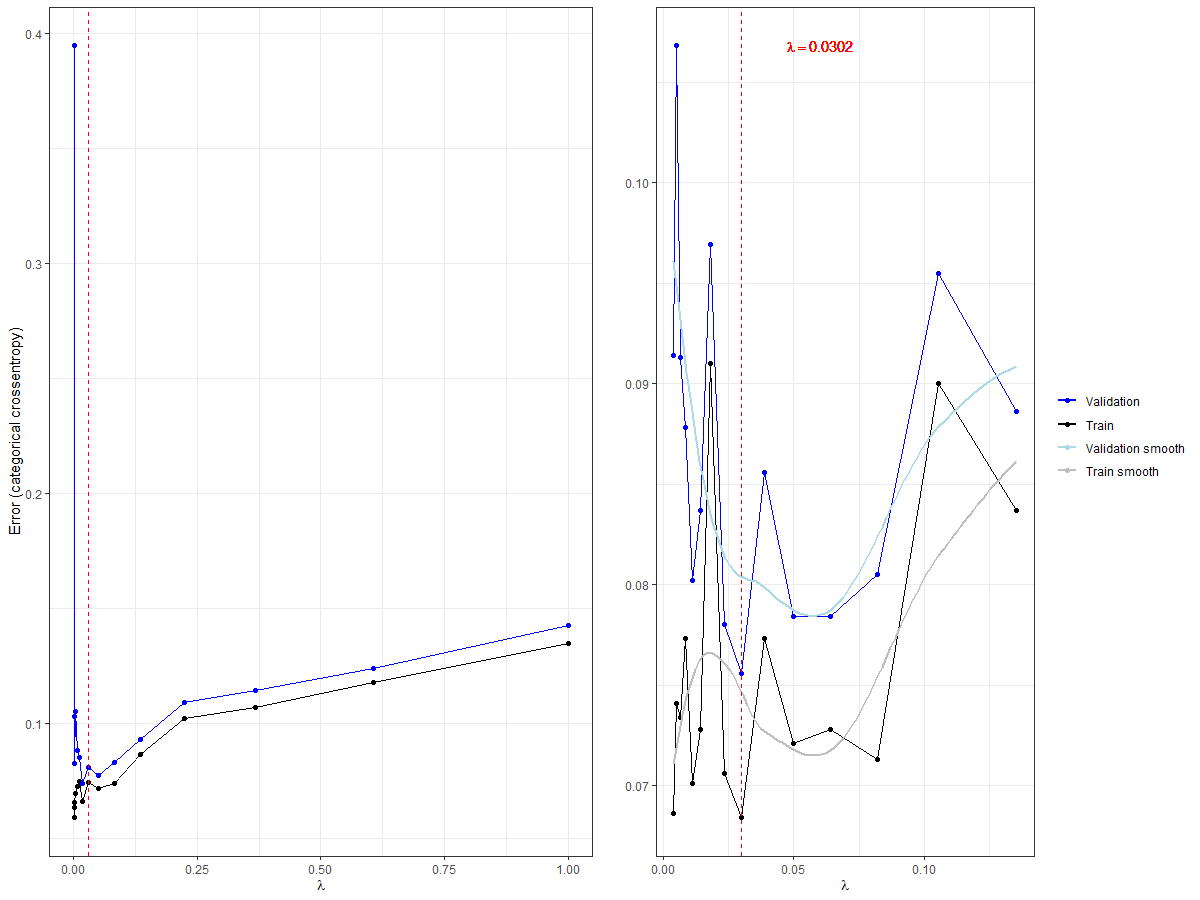
\includegraphics[scale = 0.5]{fig/CH3/all_mod_1_lambda_plot.png}
		\caption{The plot illustrates the process of selecting the best approximate $\lambda$ value for the (8)-network model applied to the combined feature data set. (left) The training and validation set errors for a range of $\lambda$ values. (right) The training and validation set errors for a more specific range of $\lambda$ values. The training and validation error smooth curves are additional curves to help view the curve patterns. Also, the $\lambda$ value that produced the minimum validation error is shown in both plots.}
		\label{fig:ch3_nn_validation_mod1_all}
	\end{center}	
\end{figure}

% validation curves NN -  (64)- all
\begin{figure}[]
	\begin{center}
		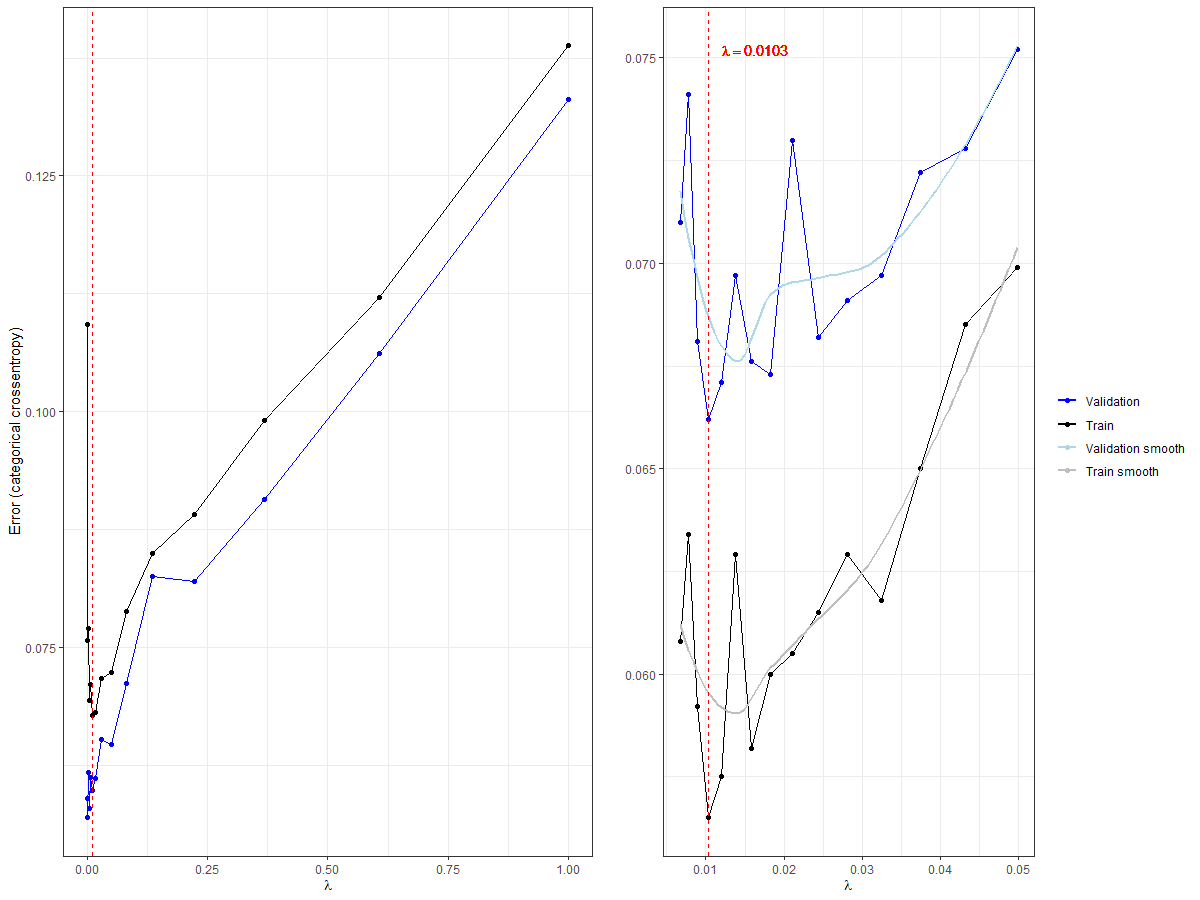
\includegraphics[scale = 0.5]{fig/CH3/all_mod_2_lambda_plot.png}
		\caption{The plot illustrates the process of selecting the best approximate $\lambda$ value for the (64)-network model applied to the combined feature data set. (left) The training and validation set errors for a range of $\lambda$ values. (right) The training and validation set errors for a more specific range of $\lambda$ values. The training and validation error smooth curves are additional curves to help view the curve patterns. Also, the $\lambda$ value that produced the minimum validation error is shown in both plots.}
		\label{fig:ch3_nn_validation_mod2_all}
	\end{center}	
\end{figure}

% validation curves comparison NN - transactional data
\begin{figure}[]
	\begin{center}
		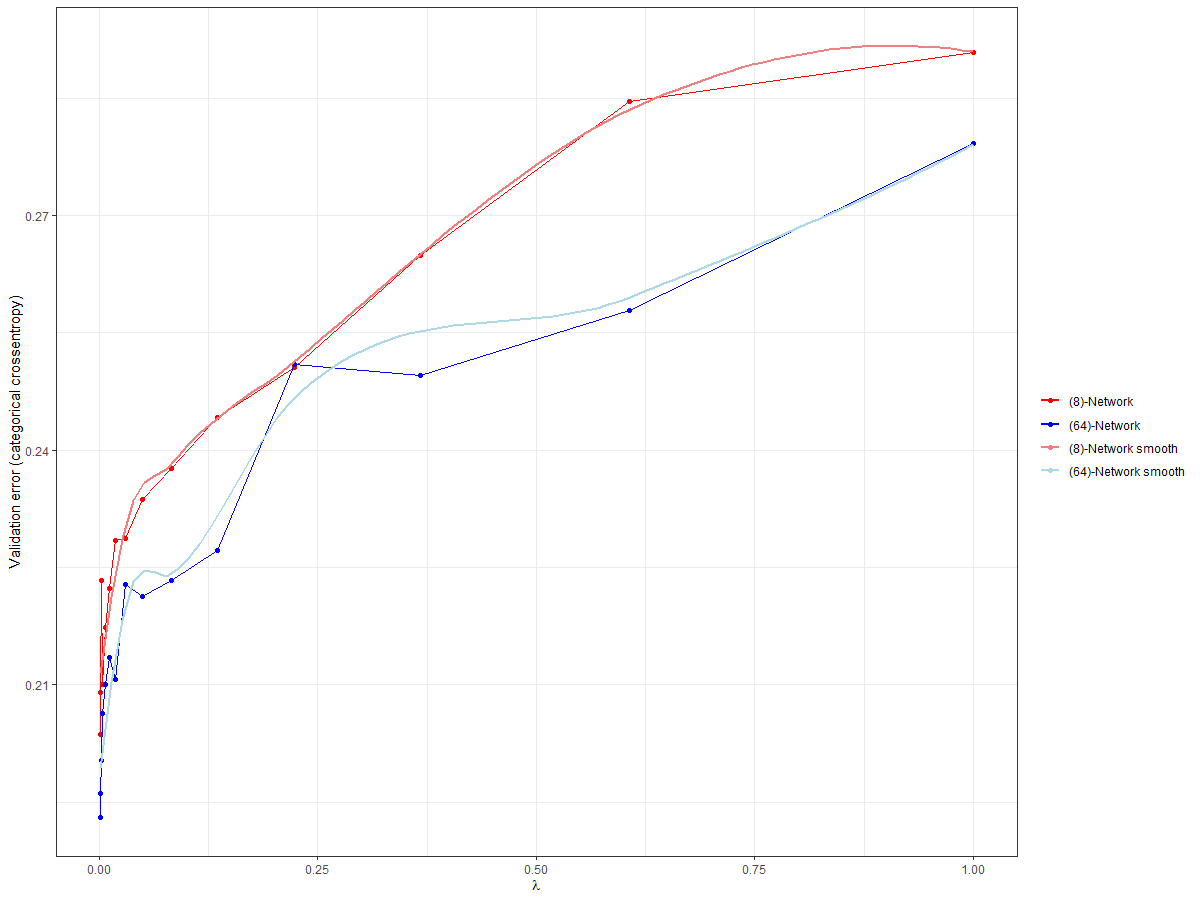
\includegraphics[scale = 0.5]{fig/CH3/model_comp_trans_HL_2.png}
		\caption{The superimposed validation error curves of the (8)-Network and (64)-Network models and their smoothing curves for $\lambda \in [0,1]$. Both models were applied to the transaction features data set.}
		\label{fig:ch3_nn_validation_compare_trans}
	\end{center}	
\end{figure}

% validation curves comparison NN - combined data
\begin{figure}[]
	\begin{center}
		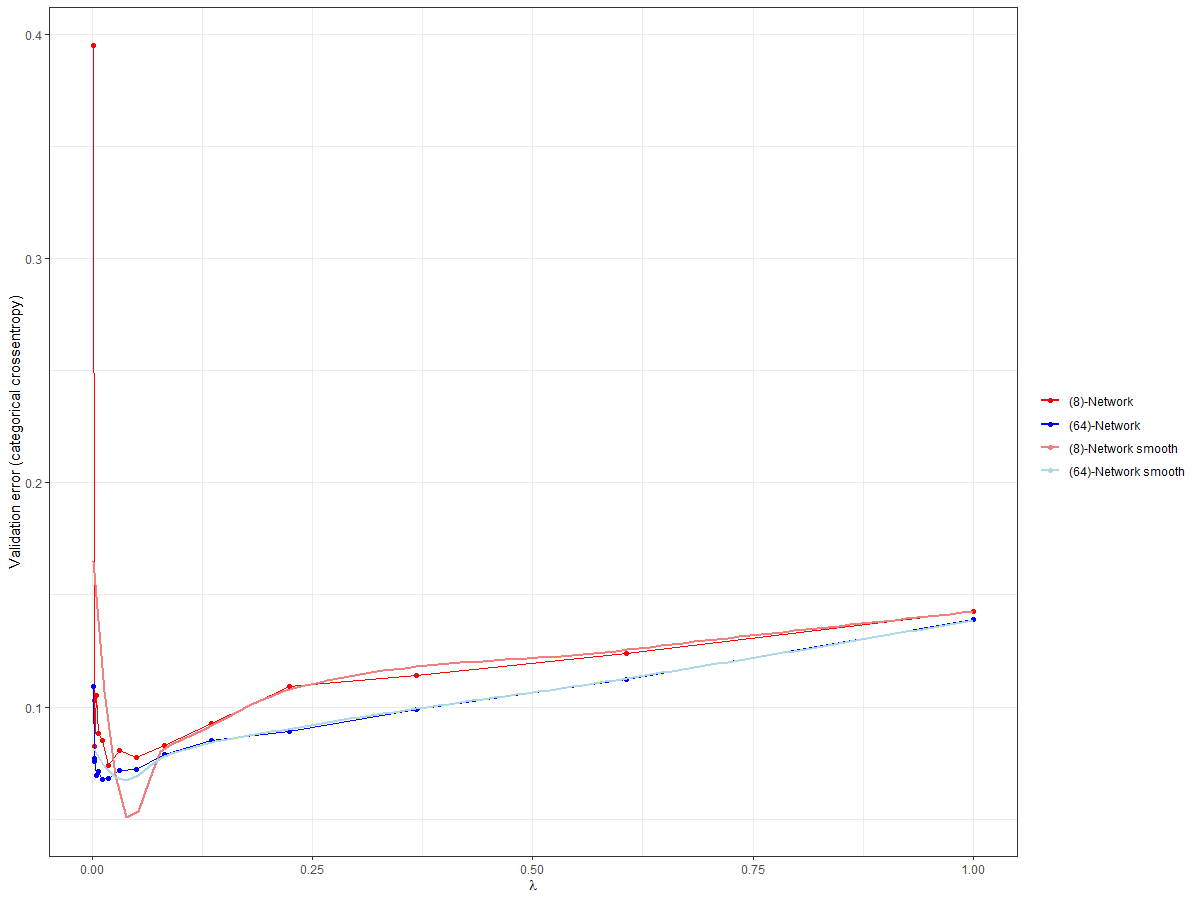
\includegraphics[scale = 0.5]{fig/CH3/model_comp_all_HL.png}
		\caption{The superimposed validation error curves of the (8)-Network and (64)-Network models and their smoothing curves for $\lambda \in [0,1]$. Both models were applied to the combined features data set.}
		\label{fig:ch3_nn_validation_compare_combined}
	\end{center}	
\end{figure}


\end{document}
